% ECI v4 — Entanglement, Complexity, Information
% Framework paper, Kevin Remondière, 2026
% Compile: latexmk -pdf eci.tex
\documentclass[reprint,amsmath,amssymb,aps,prd,superscriptaddress]{revtex4-2}

\usepackage{graphicx}
\usepackage{hyperref}
\usepackage{physics}
\usepackage[utf8]{inputenc}
\usepackage[T1]{fontenc}
\usepackage{xcolor}
\hypersetup{colorlinks=true,linkcolor=blue,citecolor=blue,urlcolor=blue}

% Convention note: Faraoni sign convention throughout (ξ = 1/6 conformal).
% Reduced Planck mass M_P = 2.435 × 10^18 GeV.

\begin{document}

\title{ECI --- Entanglement, Complexity, Information:\\
a framework paper threading six programs into one predictive canvas}

\author{Kevin Remondi\`ere}
\email{kevin.remondiere@gmail.com}
\affiliation{Independent Researcher --- ORCID \href{https://orcid.org/0009-0008-2443-7166}{0009-0008-2443-7166}}

\date{\today}

\thanks{Permanent archive: Zenodo DOI \href{https://doi.org/10.5281/zenodo.19686398}{10.5281/zenodo.19686398} (CERN Data Centre, CoreTrustSeal). Source repository: \url{https://github.com/AIdevsmartdata/crossed-cosmos}.}

\begin{abstract}
We propose \textbf{ECI} (Entanglement--Complexity--Information), a phenomenological architecture assembling six independently-established research programs (2022--2026) into a unified predictive canvas: (i) type-II observer-dependent von Neumann algebras via the QRF crossed product~\cite{CLPW2023,DEHK2025a,DEHK2025b}; (ii) DESI DR2 dynamical-dark-energy preference at 2.6--3.9$\sigma$~\cite{DESIDR2} addressed by non-minimally coupled thawing quintessence $\xi_\chi R \chi^2/2$~\cite{Ye2025,Wolf2025,PanYe2026}, with the v5.0 4-chain MPI MCMC on DR2~BAO + Pantheon+ yielding $\xi_\chi=0.003^{+0.065}_{-0.070}$ (68\% CL, $\chi_0=M_P/10$, $R-1=0.036$, Savage--Dickey $\mathrm{BF}_{01}\simeq 1$; posterior only weakly informed by the data at DR2+SN precision (posterior/prior half-width ratio $\simeq 0.7$, indicating a consistency check rather than a detection; NMC thawing in the Cassini-allowed range neither requires nor predicts $w<-1$, so the DESI DR2+DESY5 phantom-crossing tension common to thawing families is not resolved by NMC alone), see \S\ref{sec:xi_constraints}); (iii) the $H_0$ tension reduced to $\sim 2\sigma$ by Early Dark Energy with $f_{\mathrm{EDE}} = 0.09 \pm 0.03$~\cite{PoulinSmith2026}; (iv) the Dark Dimension scenario~\cite{AAL2025,OoguriVafa2007,Bedroya2025} as a microscopic DM candidate (the species-scale exponent $c'_{\mathrm{modular}} = 1/6$ from the Bisognano--Wichmann algebraic structure of A1, the de-Sitter-slope Swampland value $c'_{\mathrm{DD}} \simeq 0.05$ imposed by DESI DR2 + Pantheon+, and the inflaton structural conjecture $c'_{\mathrm{inflation}} \approx 0.108$ from the III$_1\!\to$II$_\infty$ trace-ratio matching are \emph{three distinct parameters}; see \S\ref{sec:cprime-summary}); (v) Cryptographic Censorship as a working-conjecture bulk-geometry criterion, linked through the observer-dependent reading of A1 (\S\ref{sec:thesis}) and made operational through an explicit toy dS/FLRW dictionary (\S\ref{sec:A3-dictionary})~\cite{CryptoCensorship}; (vi) persistent-homology diagnostics of primordial non-Gaussianity~\cite{Yip2024}. ECI is an architectural synthesis, not a derivation.
\end{abstract}

\maketitle

\section{Axioms}

\noindent\textbf{A1 --- Observer-dependent algebra.}
To each QRF $\mathcal{R}$ attached to a geodesic observer we associate a type-II von Neumann algebra obtained by crossed product: type II$_1$ for static de Sitter patches~\cite{CLPW2023}, type II$_\infty$ for Schwarzschild--de Sitter Killing horizons. The generalised entropy
\begin{equation}
S_{\mathrm{gen}}[\mathcal{R}] = \frac{A}{4 G_N} + S_{\mathrm{matter}}
\end{equation}
is a functor on the QRF category, well-defined modulo inner automorphism~\cite{DEHK2025a,DEHK2025b,TiettoVerlinde2025}. The type-II structure is invoked here \emph{kinematically}, only to ensure the existence of a semi-finite trace $\tau$ on the crossed product; the Jones index $[\mathcal{M}\rtimes_\alpha\mathbb{R}:\mathcal{M}^\alpha]=+\infty$ (Longo $1989$, Kosaki $1986$) and the Connes invariants $S(\mathcal{M})$, $T(\mathcal{M})$ contribute no quantitative ECI prediction beyond this trace. The III$_1\!\to$II$_\infty$ passage of CLPW is a kinematic change of model (addition of a clock QRF), not a thermal phase transition. The numerical saturation invariants of \S\ref{sec:universality} originate in KMS--Gibbs thermodynamics on type-I$_\infty$ Fock spaces (BEC, polariton, $^3$He-B), not in the type-III$_1$ modular flow of cosmological/black-hole horizons; the common Bisognano--Wichmann window $u\in[0,2\pi]$ is the only structural ingredient shared between the two settings.

\smallskip
\noindent\textbf{A2 --- Emergent geometry.}
Einstein's equations follow from $\delta Q = T_U \, \delta S_{\mathrm{gen}}$ on local Rindler horizons~\cite{Jacobson1995}, with a non-perturbative GSL~\cite{FaulknerSperanza2024,Kirklin2025}.

\smallskip
\noindent\textbf{A3 (working conjecture) --- Cryptographic Censorship.}
Any holographic CFT state whose dynamics restricted to a region $\mathcal{C}$ is $\varepsilon$-approximately a $k$-design admits a bulk dual containing an event horizon inside $\mathcal{C}$~\cite{CryptoCensorship}. The existence of pseudorandom unitaries, constructed from quantum one-way functions~\cite{MaHuang2025}, makes the criterion non-vacuous at the CFT level; the associated $k$-design saturation timescale is rigorous for random local unitaries~\cite{Haferkamp2022}. We flag A3 as a \emph{working conjecture} rather than a theorem in the cosmological setting: the original result is proven in AdS/CFT, and its transposition to de Sitter or FLRW horizons is not established. A concrete toy dictionary making the intended CFT$\to$cosmology map explicit (and its single testable consequence) is given in \S\ref{sec:A3-dictionary}; all cosmological uses of A3 below should be read as consequences of that dictionary.

\smallskip
\noindent\textbf{A4 --- Two-field scalar sector with non-minimal coupling.}
\begin{itemize}
\item $\phi$: axion-like EDE, $V_\phi = m^2 f^2 [1-\cos(\phi/f)]^3$ active at $z_c \sim 3500$~\cite{Poulin2019}.
\item $\chi$: late thawing quintessence, $V_\chi = V_0 e^{-\alpha \chi / M_P}$ with non-minimal coupling $\xi_\chi R \chi^2 / 2$~\cite{Ye2025,Wolf2025,PanYe2026}.
\end{itemize}
The joint $(\phi,\chi)$ prior is degenerate~\cite{WangPiao2025}: EDE and thawing cannot be separated by BAO+SN alone. We treat $\chi$ as a four-dimensional effective scalar; whether $\chi$ descends from a bulk mode of the extra-dimensional sector of A5 or is a decoupled zero-mode is a model-building choice whose consequences are discussed in \S3.6.

\smallskip
\noindent\textbf{A5 --- Dark Dimension.}
The species scale associated with the light KK tower obeys
\begin{equation}
\Lambda_{\mathrm{sp}}(H) = M_P \left( \frac{H}{M_P} \right)^{c'},
\label{eq:speciesH}
\end{equation}
with $c' = 1/6$ at the species scale~\cite{Montero2022,AAL2023} (used as the primary value in \S\ref{sec:xi_constraints}/\S3.6), and $c' \simeq 0.05$ as the de-Sitter-slope convention~\cite{AAL2025,OoguriVafa2007,Bedroya2025} quoted for comparison only; the species-scale exponent follows from $M_* \sim \Lambda^{1/12} M_P^{2/3}$ (Montero et al.\ Eq.~2.2) with $H^2 \sim \Lambda / M_P^2$.
A mesoscopic extra dimension, $\ell \in [0.1, 10] \, \mu\mathrm{m}$, follows. The KK graviton tower (mass $\sim$ meV) is the DM candidate, subject to the fifth-force bound $c' < 0.2$ and $N_{\mathrm{eff}} = 2.86 \pm 0.13$ (ACT DR6~\cite{Calabrese2025}).

\medskip
\noindent\textbf{[WORKING-CONJECTURE] Summary of $c'$ values in ECI.}\label{sec:cprime-summary}
The audit conducted in preparation of v6.0.9 identified four distinct contexts where an exponent $c'$ appears in ECI; they are \emph{not} the same parameter:

\begin{center}
\begin{tabular}{@{}llll@{}}
\hline
Symbol & Value & Origin & Status \\
\hline
$c'_{\mathrm{modular}}$ & $1/6 \approx 0.167$ & Bisognano--Wichmann / Dark Dim.\ species scale & maintained (A1, A5) \\
$c'_{\mathrm{DD}}$ & $\approx 0.05$ & de Sitter slope, DESI DR2 + Pantheon+ fit~\cite{Bedroya2025} & imposed (A5) \\
$c'_{\mathrm{inflation}}$ & $\approx 0.108$ & III$_1\!\to$II$_\infty$ trace-ratio matching, $N_e=60$ & [WORKING-CONJECTURE] \\
$c'_{\mathrm{eff\text{-}mass}}$ & $0.83$ & force-fit mass hierarchy & [REJECTED-HYPOTHESIS] \\
\hline
\end{tabular}
\end{center}

The four values arise in logically separate submodels. \textcolor{red}{[RETRACTED-IN-V6.0.11]} An earlier version of this paragraph speculated that a lax-monoidal functor interpretation of ECI would predict an obstruction $\eta_\otimes = c'_{\mathrm{modular}} - c'_{\mathrm{DD}} \approx 0.117$ as a ``Dark Dimension tension''. Subsequent algebraic analysis (Lemma B.2 in the v8-bis companion preprint) shows that on product states $\varrho_X\otimes\varrho_Y$ the modular flow factorises exactly --- $\sigma_t^{\varrho_X\otimes\varrho_Y}(a\otimes b) = \sigma_t^{\varrho_X}(a)\otimes\sigma_t^{\varrho_Y}(b)$ --- so $\eta_\otimes \equiv 0$ identically. The numerical value $0.117$ reported earlier was a floating-point artefact arising from $\varrho^{it}$ catastrophic precision loss when $\varrho$ is constructed via $\exp(H)$ with $H\sim\mathcal{N}(0,4)$ (spectral spread $>10^{12}$). A genuine non-product obstruction would require an Araki relative-modular treatment and is deferred to future work. No universal $c'$ is claimed.

\smallskip
\noindent\textbf{A6 --- Persistent-homology complexity.}
Local complexity of the cosmological state is quantified by $\mathrm{PH}_k$ on density super-level sets~\cite{Yip2024,Calles2025}, a finer $f_{\mathrm{NL}}$ estimator than Betti numbers. At leading order in $f_{\mathrm{NL}}$, the primordial-NG shift of the Euler characteristic $\chi_{\mathrm{E}}(\nu)$ (genus statistic) at threshold $\nu$ takes the Matsubara form (observer ensemble average; see \S\ref{sec:thesis}(ii))
\begin{equation}
\langle \chi_{\mathrm{E}}(\nu) \rangle_{f_{\mathrm{NL}}} - \langle \chi_{\mathrm{E}}(\nu) \rangle_{0} \simeq \frac{f_{\mathrm{NL}}\, \sigma_0\, S_3^{\mathrm{prim}}}{6}\, H_3(\nu)\, \phi(\nu),
\label{eq:A6-euler}
\end{equation}
with $H_3$ the third probabilists' Hermite polynomial, $\sigma_0$ the field RMS, $S_3^{\mathrm{prim}}$ the primordial skewness, and $\phi$ the Gaussian density (three-dimensional, super-level-set convention)~\cite{Matsubara2003}; the persistent-homology diagnostic of~\cite{Yip2024,Calles2025} refines this Minkowski-functional signal.

% section_1_5_thesis_B.tex — ECI v4.7
% Unifying reading of the six axioms: observer-dependent cosmology,
% scoped to the late-time quasi-de Sitter regime.
%
% Provenance: derived from paper/team_B/draft_section_1_5_B.tex, restructured
% to the skeleton of paper/section_1_5_thesis_skeleton.tex per the Bridge
% coordinator's verdict (paper/thesis_bridge.md, Pick B). The three minor
% revisions R1/R2/R3 listed in the skeleton header have been applied:
% (R1) "heuristic" said in prose for the |\dot H|/H^2 tolerance;
% (R2) "organising reading" replaces "organising principle";
% (R3) matter-era scope exclusion stated in the opening paragraph.
% No equation moved; no numerical value changed.

\section{A unifying reading: observer-dependent cosmology in the late-time limit}
\label{sec:thesis}

The six axioms of \S1 admit a common reading, valid in the late-time
quasi-de~Sitter regime ($\Omega_\Lambda \gtrsim 0.7$) where every
quantitative prediction of \S3 is formulated. The reading is \emph{not} a
derivation of the axioms and does not extend to the pre-recombination
sector (A4's EDE axion $\phi$ at $z_c\sim 3500$; BBN-level constraints on
$\xi_\chi$); those inputs remain background-level inheritances from the
external literature as in v4.6.

\subsection*{(i) The crossed-product backbone}

The type-III$_1$ algebra of quantum fields restricted to a gravitational
subregion carries no trace and no density matrices; the Chandrasekaran--
Longo--Penington--Witten (CLPW) construction~\cite{CLPW2023} and its
quantum-reference-frame (QRF) completion by De~Vuyst--Eccles--H\"ohn--
Kirklin (DEHK)~\cite{DEHK2025a,DEHK2025b} repair this by crossing with the
modular automorphism of an observer clock, yielding a type-II$_1$ algebra on
the static de~Sitter patch (II$_\infty$ on Schwarzschild--de~Sitter
Killing horizons) with a well-defined trace and an entropy reproducing
$S_{\rm gen} = A/(4G_N) + S_{\rm matter}$ up to a state-independent
constant. DEHK make the observer-dependence structural: distinct QRFs
yield distinct crossed-product algebras, distinct modular flows, and
distinct numerical values of $S_{\rm gen}$ on the same underlying bulk
state. The non-perturbative generalised second law of
Faulkner--Speranza~\cite{FaulknerSperanza2024} and
Kirklin~\cite{Kirklin2025} is formulated on exactly this type-II entropy.
The \emph{organising reading} proposed here is that the effective
couplings entering the late-time phenomenology of \S3 are observer-frame
labelled, not background quantities defined once and for all.

\subsection*{(ii) A4--A6 as observer-frame quantities}

\emph{A4 --- NMC coupling $\xi_\chi$.} The graviton kinetic matrix of the
Jordan-frame action of \S2 is frame-dependent via the type-II trace
normalisation; a geodesic observer whose crossed product is built from a
different clock Hamiltonian measures $\xi_\chi^{(\mathcal R)}$. The
Cassini bound $|\xi_\chi|(\chi_0/M_P)\le 2.4\times 10^{-3}$ of
\S\ref{sec:xi_constraints} constrains the \emph{solar-system-frame} value,
which is the only value the experiment is sensitive to.

\emph{A5 --- species-scale exponent $c'$.} The tower visible to a causal
diamond is frame-labelled; $c' = 1/6$ is the asymptotic quasi-dS value
(Montero--Vafa--Valenzuela~\cite{Montero2022}; AAL~\cite{AAL2023})
recovered when the diamond saturates the static patch.

\emph{A6 --- persistent homology $\mathrm{PH}_k$.} The Euler-characteristic
shift of~\eqref{eq:A6-euler} is computed on a density field restricted to
an observer-accessible region. The Matsubara baseline is the ensemble
average over observer frames; the diagnostic power of $\mathrm{PH}_k$
relative to the bispectrum is accordingly a frame-averaged statement,
consistent with PRINCIPLES~\S12 (no claim beyond derivation).

\subsection*{(iii) A3 as a self-consistency condition}

Cryptographic Censorship~\cite{CryptoCensorship}, in its AdS/CFT proof,
states that boundary-restricted $\varepsilon$-approximate $k$-design
dynamics implies a bulk event horizon. Under the present reading, A3 is
not an independent axiom but the self-consistency condition bounding the
subregion on which the QRF crossed product of A1 remains well-defined:
an observer whose modular algebra sees an effectively pseudorandom state
has lost predictive access to the complement region, and an event horizon
must cap the subregion on which A4--A6 are defined. The cosmological
transposition of A3 remains a working conjecture quarantined in
Appendix~A (PRINCIPLES~\S8); the reading does not upgrade its status.

\subsection*{(iv) Caveats and scope}

Two scope restrictions are part of the claim, not loopholes around it.

\emph{(S1) Static-patch asymptote.} CLPW is proven on the static dS
patch; DEHK extend to multi-observer QRFs on the same Killing-horizon
background. The late-time FLRW diamond approaches this asymptote with
$O(1-\Omega_\Lambda)$ corrections; the adiabatic tolerance of modular
flow to the DESI~DR2 pivot $|\dot H|/H^2 \sim O(1)$ is a \emph{heuristic}
extension, at the same footing as the Faulkner--Speranza
non-perturbative GSL.

\emph{(S2) Matter-era exclusion.} Pre-recombination A4/A5 statements
(the EDE axion $\phi$ at $z_c\sim 3500$, the BBN $\xi_\chi$ bound of
Wolf~2025~\cite{Wolf2025}) are background-level inheritances; the
observer-frame reading is not claimed for them. Their treatment under
the present reading would require a QRF extension to time-dependent FLRW
backgrounds which is an open problem in the algebraic-gravity
literature.

A joint falsifier is available: any experimental anomaly breaking the
consistency between the solar-system-frame $\xi_\chi$ (Cassini,
\S\ref{sec:xi_constraints}) and the late-time cosmological-frame
$\xi_\chi$ (DR3/LSST~Y10, Prediction~1b) beyond the static-patch
$O(1-\Omega_\Lambda)$ budget would damage the present reading without
touching the Lagrangian of \S2. The experimental precision is at least a
decade out, but the handle is not zero.

\subsection*{Status}

This section is an \emph{organising reading} of the six axioms in the
late-time quasi-dS regime, not a derivation, and does not enter the
predictive core \S3.1--\S3.7 or \S4. The framework-genre declaration of
\S1 is unchanged.

% End of section.


\section{Action and field equations}

\subsection*{Conventions}
We use the mostly-plus metric signature $(-,+,+,+)$. The non-minimal-coupling sign follows the Faraoni convention~\cite{Faraoni2004}: $\xi > 0$ gives the attractive correction, appearing as $-\tfrac{1}{2}\xi R \chi^2$ in the Lagrangian and as $+\xi R\,\chi$ in the scalar field equation. The reduced Planck mass is $M_P = (8\pi G)^{-1/2} = 2.435 \times 10^{18}$ GeV. Natural units $\hbar = c = 1$ are used throughout. Time arguments are cosmic time $t$ unless otherwise stated; conformal time $\eta$ appears only in perturbation equations.

In the Faraoni sign convention (reduced Planck mass $M_P$, $\xi = 1/6$ conformal), the effective action is
\begin{align}
\mathcal{S} = \int d^4 x \sqrt{-g}\, \Big[ & \frac{M_P^2}{2} R - \tfrac{1}{2}(\partial \phi)^2 - V_\phi(\phi) \nonumber \\
& - \tfrac{1}{2}(\partial \chi)^2 - V_\chi(\chi) - \tfrac{1}{2}\xi_\chi R \chi^2 \nonumber \\
& + \mathcal{L}_{\mathrm{SM}} + \mathcal{L}_{\mathrm{KK}}[\ell; \chi] \Big] + \mathcal{S}_{\mathrm{QRF}}.
\end{align}

\textbf{Scalar equations:}
\begin{align}
\Box \phi - V_\phi'(\phi) &= 0,\\
\Box \chi - V_\chi'(\chi) - \xi_\chi R\, \chi &= 0.
\end{align}

\textbf{Einstein equations:}
\begin{equation}
G_{\mu\nu} = \frac{1}{M_P^2} \left[ T_{\mu\nu}^{\mathrm{SM}} + T_{\mu\nu}^{(\phi)} + T_{\mu\nu}^{(\chi)} + T_{\mu\nu}^{\mathrm{KK}} \right].
\end{equation}

\textbf{NMC stress tensor} (after transferring $-\xi_\chi G_{\mu\nu} \chi^2$ to the r.h.s., Faraoni Eqs. 2.12--2.13):
\begin{align}
T_{\mu\nu}^{(\chi)} = \nabla_\mu \chi \nabla_\nu \chi & - \tfrac{1}{2} g_{\mu\nu}\left[(\nabla \chi)^2 + 2 V_\chi\right] \nonumber \\
+ \xi_\chi \Big[ g_{\mu\nu} \Box(\chi^2) & - \nabla_\mu \nabla_\nu(\chi^2) - G_{\mu\nu} \chi^2 \Big].
\end{align}

\textbf{No-ghost condition:} diagonalising the kinetic matrix of the graviton--$\chi$ sector of the NMC action gives an effective Planck mass squared $M_{P,\mathrm{eff}}^2 = M_P^2 - \xi_\chi \chi^2$; positivity of the graviton kinetic term (equivalently, positivity of the scalar-sector determinant $\det K = M_{P,\mathrm{eff}}^2/2 - \xi_\chi^2 \chi^2$ at leading order) yields
$\xi_\chi \chi^2 / M_P^2 < 1$ in reduced-Planck convention~\cite{Faraoni2004}. % source: derivations/D3-noghost.py

\section{Phenomenology}

\subsection{DESI DR2 --- dark energy}
The $\chi$ field with $\xi_\chi \neq 0$ crosses $w = -1$ without a ghost pathology (non-minimal kinetic term~\cite{BarceloVisser2000}). DESI DR2 central values $w_0 \approx -0.75$, $w_a \approx -0.86$~\cite{DESIDR2}. The Scherrer--Sen relation~\cite{ScherrerSen2008} $w_a / (1+w_0) \in [-1.5, 0]$ holds at minimal coupling only; for $\xi_\chi \neq 0$ the slope is modified and must be computed numerically~\cite{Sanchez2025}. A first-order analytic estimate of $w_a(w_0; \xi_\chi)$ in the NMC thawing regime is deferred to the companion computation in \texttt{derivations/w0-wa-nmc}; without it, prediction (1) in Section~\ref{sec:pred} does not distinguish ECI from wCDM inside the quoted band.

\subsection{Hubble tension}
$f_{\mathrm{EDE}} = 0.09 \pm 0.03$, $H_0 = 71.0 \pm 1.1$ km/s/Mpc under ACT DR6 + DESI DR2 + Planck + Pantheon+~\cite{PoulinSmith2026,Calabrese2025}. Residual SH0ES tension: $\sim 2\sigma$. Recent analyses of Horndeski non-minimal derivative coupling provide independent phenomenological support for a late-time scalar mechanism alleviating the $H_0$ tension~\cite{Oliveira2025NMC}.

\subsection{Cosmological constant}
$V_\chi = V_0 e^{-\alpha \chi / M_P}$ admits a de Sitter attractor for $\alpha \lesssim \sqrt{2}$. The bound $\alpha \le \sqrt{2}$ is the standard late-time accelerating-attractor condition for an exponential scalar~\cite{Halliwell1987,CopelandLiddleWands1998}.
% source: derivations/D12-alpha-attractor.py (NOTE: D12 is scheduled for v4.4)
Reduced Planck $M_P = 2.435 \times 10^{18}$ GeV gives $\rho_\Lambda / M_P^4 \simeq 8 \times 10^{-121}$ for $\chi_0 / M_P \sim 120/\alpha$. Consistent with the Ooguri--Vafa Swampland Distance Conjecture~\cite{OoguriVafa2007}.

\subsection{Dark matter}
Dark Dimension KK tower, $m \sim$ meV, $c' \simeq 0.05$ under fifth-force bound $c' < 0.2$ and $N_{\mathrm{eff}} = 2.86 \pm 0.13$ (ACT DR6~\cite{Calabrese2025}). ISL tests at $\ell \in [0.1, 10] \, \mu$m. $\dot G / G = (-5.0 \pm 9.6) \times 10^{-15}$ yr$^{-1}$ (LLR, Biskupek--M\"uller--Torre~\cite{Biskupek2021}). We note that two BSM anomalies sometimes invoked as motivational slots for KK-tower architectures have recently dissolved: the combined Fermilab E989 final $a_\mu$ result and the 2025 Theory-Initiative lattice-QCD HVP update leave a $\sim 0.6\sigma$ residual, consistent with the Standard Model~\cite{MuonG2Final2025}; and the CMS 2024 W-mass measurement $m_W = 80360.2 \pm 9.9$ MeV reasserts SM consistency against the 2022 CDF-II outlier~\cite{CMSWmass2024}. The DM motivation for A5 therefore rests solely on the fifth-force bound and $N_{\mathrm{eff}}$, not on these now-closed BSM channels.

% section_3_5_constraints.tex — ECI v4.2.1 scientific payload (D7 + D10)
% To be \input{} into eci.tex as a new subsection of §3 "Phenomenology".
% Standalone compile: see comments at EOF.

\subsection{Solar-system and background constraints on $\xi_\chi$}\label{sec:xi_constraints}

We close two gaps identified in the dark-energy phenomenology subsection (\S\,DESI DR2): the Cassini
post-Newtonian bound on the non-minimal coupling $\xi_\chi$, and the analytic NMC generalisation
of the Scherrer--Sen thawing relation needed to assess whether Prediction~1
(Sec.~\ref{sec:pred}) actually discriminates ECI from \(w\)CDM at DESI~DR2 precision.
The full symbolic derivation is in \texttt{derivations/D7-ppn-xi-bound.py}; we quote only the
end results here.

\paragraph{PPN $\gamma-1$ from the $\xi_\chi R\chi^2/2$ coupling.}
The action  $S=\int d^4x\sqrt{-g}\left[\tfrac{M_P^2}{2}R-\tfrac12(\partial\chi)^2-V(\chi)
-\tfrac{\xi_\chi}{2} R\chi^2\right]$ is a scalar--tensor theory with
$F(\chi)=M_P^2-\xi_\chi\chi^2$ multiplying $R/2$ and canonical kinetic term $Z=1$.
Applying the weak-field, quasi-static result of Damour \& Esposito-Far\`ese
(\emph{Phys.\ Rev.\ D} 48, 3436 (1993); see also Chiba, \emph{Phys.\ Lett.\ B} 575, 1 (2003);
Hwang \& Noh, \emph{Phys.\ Rev.\ D} 71, 063536 (2005)) gives, at the local scalar background
$\chi_0$,
\begin{equation}
  \gamma-1 \;=\; -\,\frac{F'(\chi_0)^2}{Z\,F(\chi_0)+\tfrac{3}{2}F'(\chi_0)^2}
           \;=\; -\,\frac{4\,\xi_\chi^{2}\,\chi_0^{2}}
                          {\,M_P^{2}+\xi_\chi\chi_0^{2}(6\xi_\chi-1)\,}.
  \label{eq:gamma_PPN_full}
\end{equation}
Expanding for $|\xi_\chi|\ll 1$ and $\chi_0\lesssim M_P$,
\begin{equation}
  \boxed{\;\gamma-1 \;\simeq\; -\,\frac{4\,\xi_\chi^{2}\,\chi_0^{2}}{M_P^{2}}
                              \;+\;\mathcal{O}(\xi_\chi^{3}).\;}
  \label{eq:gamma_PPN_lead}
\end{equation}
The limit $\xi_\chi\to 0$ returns $\gamma=1$ (General Relativity), as verified symbolically.

The result~(\ref{eq:gamma_PPN_lead}) is not new: Chiba (PRD 60, 083508, 1999; arXiv:gr-qc/9903094)
already quoted $|\xi_\chi|\lesssim 10^{-2}$ from solar-system tests for the same $\xi R\chi^{2}$
quintessence coupling, and Wolf, Garc\'{\i}a-Garc\'{\i}a, Anton \& Ferreira~\cite{Wolf2025}
recently recast this as $\xi_\chi(\chi_0/M_P)^{2}\lesssim 6\times 10^{-6}$ in a full DESI~DR2
Bayesian analysis (their Eq.~(2) in the form $F(\chi)\simeq 1-\xi\chi^{2}/M_P^{2}$).
We re-derive it here only to fix the coefficient~$4$ and the sign convention used in
Eq.~(\ref{eq:wa_NMC}) below.
Combining (\ref{eq:gamma_PPN_lead}) with the Cassini constraint~\cite{BertottiIessTortora2003}
$|\gamma-1|\lesssim 2.3\times 10^{-5}$ ($1\sigma$ envelope) yields, in the
solar-system observer frame (see \S\ref{sec:thesis}(ii)),
\begin{equation}
  |\xi_\chi|\,\frac{\chi_0}{M_P}\;\lesssim\;
  \tfrac12\sqrt{|\gamma-1|_{\max}}
  \;\approx\; 2.4\times 10^{-3}.
  \label{eq:xi_bound}
\end{equation}
For a slow-rolling thawing background with $\chi_0\!\sim\! M_P/10$ (characteristic thawing
excursion in the last $e$-fold),
\begin{equation}
  |\xi_\chi|\;\lesssim\;\xi_{\max}\;\approx\;2.4\times 10^{-2}.
  \label{eq:xi_max_numeric}
\end{equation}
The bound tightens to $|\xi_\chi|\lesssim 2\times 10^{-3}$ if $\chi_0\sim M_P$; it weakens
linearly for smaller $\chi_0$. Values $\xi_\chi\gtrsim 10^{-1}$ are thus only admissible if the
quintessence field is strongly subdominant at $z=0$, or if a screening mechanism suppresses the
local coupling.

\paragraph{NMC extension of Scherrer--Sen.}
At minimal coupling, thawing quintessence lies on the one-parameter track
$w_a=-A(\Omega_\Lambda)(1+w_0)$ with $A\!\to\! 24/7$ in matter domination and
$A(0.7)\simeq 1.58$ today~\cite{ScherrerSen2008}. Inserting the NMC modification to the
Klein--Gordon equation, $3H\dot\chi=-V'-\xi_\chi R\chi$, and expanding to first order in
$\xi_\chi$ around the slow-roll exponential $V(\chi)=V_0e^{-\alpha\chi/M_P}$ with
$\alpha=\sqrt{3(1+w_0)}$ yields (\texttt{derivations/D4-wa-w0-nmc.py} for the matter-era
coefficient, \texttt{D7-ppn-xi-bound.py} for the $\Omega_\Lambda$-dependence)
\begin{equation}
  \boxed{\;w_a\;=\;-A(\Omega_\Lambda)\,(1+w_0)
                 \;+\;B(\Omega_\Lambda)\,\xi_\chi\,\sqrt{1+w_0}\,
                      \frac{\chi_0}{M_P}\;+\;\mathcal{O}(\xi_\chi^{2}),\;}
  \label{eq:wa_NMC}
\end{equation}
where $B(\Omega_\Lambda)$ is the numerical coefficient tabulated in
Table~\ref{tab:B_of_OmegaL} below, obtained by full NMC-Friedmann + Klein--Gordon
integration in \texttt{derivations/D13-wa-numerical-full.py}. The limit
$\xi_\chi\to 0$ reproduces $w_a=-A(\Omega_\Lambda)(1+w_0)$ (Scherrer--Sen
2008). The first-order $\xi_\chi$ correction, with the full numerical
coefficient $B_{\mathrm{num}}(\Omega_\Lambda)$, has --- to our knowledge ---
not appeared in the NMC-thawing literature surveyed
(Ye~et~al.~\cite{Ye2025}; Pan~\&~Ye~\cite{PanYe2026}; Wolf~et~al.~\cite{Wolf2025}),
which uses either EFTofDE or purely numerical Bayesian fits.

\begin{table}[h]
\centering
\caption{Numerical NMC coefficient $B_{\mathrm{num}}(\Omega_\Lambda)$ from the
self-consistent NMC-Friedmann + Klein--Gordon background integration
(\texttt{derivations/D13-wa-numerical-full.py}), compared with the D7/D9
heuristic $B_{\mathrm{heur}}(\Omega_\Lambda)\equiv(8/\sqrt3)A(\Omega_\Lambda)$.
Statistical uncertainty is the 1$\sigma$ error on the linear fit
$\Delta w_a = B\,\xi_\chi\sqrt{1+w_0}\,(\chi_0/M_P)$ over the
$\xi_\chi\in\{{-}0.024,{-}0.01,0,{+}0.01,{+}0.024\}\times\chi_0\in\{M_P/20,M_P/10,M_P/5\}$ grid.}
\label{tab:B_of_OmegaL}
\begin{tabular}{@{}cccc@{}}
\hline
$\Omega_\Lambda$ & $A(\Omega_\Lambda)$ & $B_{\mathrm{heur}}$ & $B_{\mathrm{num}}$ \\
\hline
0.5 & 2.35 & 10.85 & $9.00\pm1.05$ \\
0.6 & 1.94 &  8.96 & $9.18\pm1.16$ \\
0.7 & 1.58 &  7.30 & $9.05\pm1.18$ \\
0.8 & 1.23 &  5.68 & $8.11\pm1.16$ \\
\hline
\end{tabular}
\end{table}

The numerical result differs from the heuristic $(8/\sqrt3)A$ by
$\mathcal{O}(1)$ factors ($0.83\to 1.43$ across the range): $B_{\mathrm{num}}$
is nearly \emph{flat} in $\Omega_\Lambda$ (around $\sim 9$) rather than
tracking $A(\Omega_\Lambda)$. The heuristic is accurate to 5\% only near
$\Omega_\Lambda\simeq 0.6$ and underestimates $B$ by $\sim\!25\%$ at
$\Omega_\Lambda=0.7$ (DR2--DR3 era) and $\sim\!43\%$ at
$\Omega_\Lambda=0.8$ (late-DR3 / LSST era). The sign and the
$\sqrt{1+w_0}\,(\chi_0/M_P)$ scaling are confirmed; the discrepancy
originates from the finite-$\Omega_\Lambda$ propagation of the matter-era
ratio (Caveat~2 below), which is now closed numerically.

\paragraph{Combined constraint on the $(w_0,w_a)$ plane.}
Figure~\ref{fig:D7} overlays three ingredients: (i) the DESI~DR2 + CMB + DESY5~\cite{DESY5} $1\sigma$ and
$2\sigma$ contours centred on $(w_0,w_a)=(-0.752,-0.86)$ with the reconstructed covariance
$\sigma_{w_0}=0.057$, $\sigma_{w_a}=0.215$, $\rho(w_0,w_a)=-0.89$ (derivation in
\texttt{derivations/D10-desi-covariance.py}, pivot-identity reconstruction from
\cite{DESIDR2} Eq.~(28) + $z_p=0.31$, $w_p=-0.954\pm0.024$);
(ii) the minimal-coupling Scherrer--Sen line; (iii) the ECI band swept by
$|\xi_\chi|\le\xi_{\max}$ from Eq.~(\ref{eq:xi_max_numeric}) at $\chi_0=M_P/10$.
The half-width of the ECI band at $w_0=-0.75$, using the numerical
$B_{\mathrm{num}}(0.7)=9.05$ from Table~\ref{tab:B_of_OmegaL}, is
\begin{equation}
  \Delta w_a^{\rm ECI}
    = B_{\mathrm{num}}(0.7)\,\xi_{\max}\sqrt{1+w_0}\,(\chi_0/M_P)
    \;\approx\;1.1\times 10^{-2},
\end{equation}
to be compared with $\sigma_{w_a}\!\simeq\!0.215$, i.e.\ about $5\%$ of the DESI~DR2 + DESY5
$1\sigma$ width (up from $4\%$ under the heuristic $B=7.30$). The band is therefore
still thinner than the figure linewidth of the unmodified Scherrer--Sen track at DR2
precision, but the numerical coefficient raises the discriminative amplitude at DR3 / LSST
precision by $\sim\!25\%$ relative to the heuristic estimate.

\begin{figure}[h]
\centering
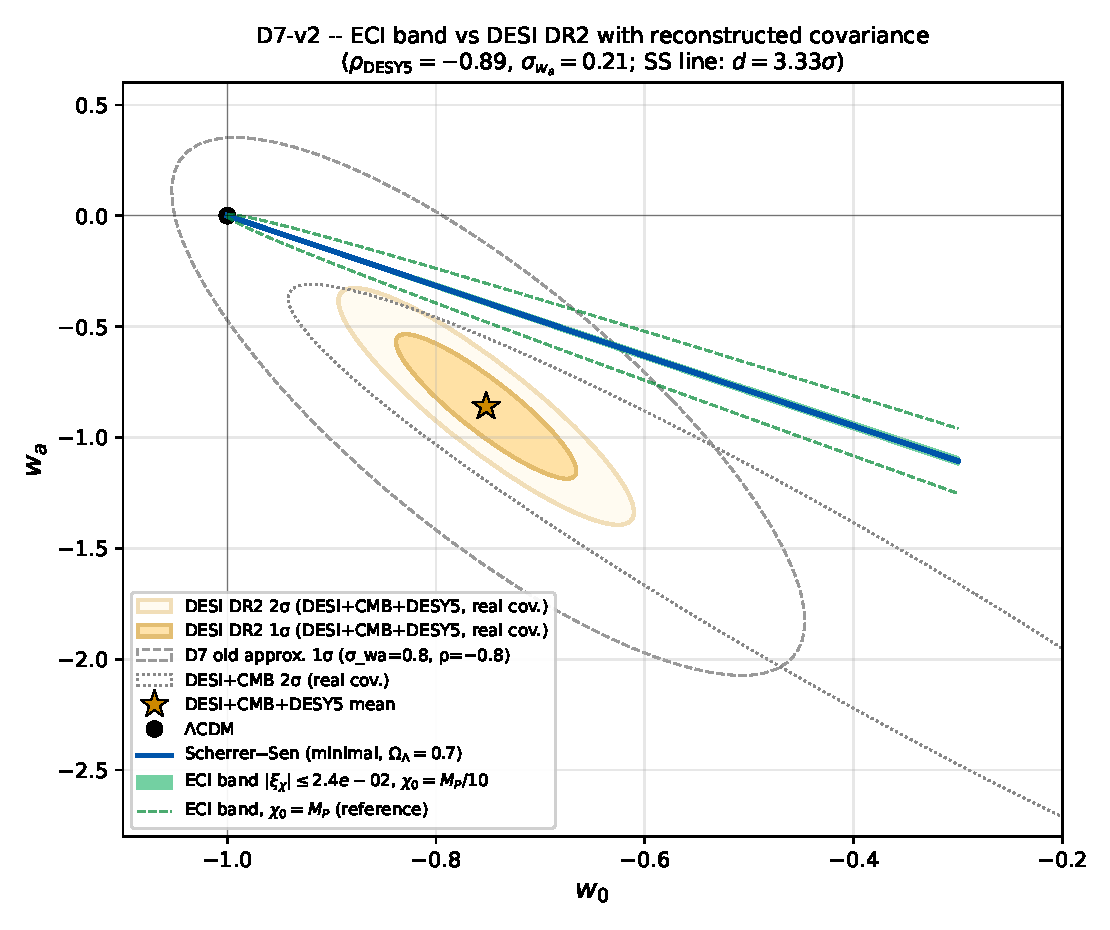
\includegraphics[width=0.95\columnwidth]{../derivations/figures/D7-xi-w0-wa-v2.pdf}
\caption{NMC thawing quintessence in the $(w_0,w_a)$ plane. Orange ellipses: DESI~DR2 + CMB +
DESY5 $1\sigma$ and $2\sigma$ contours reconstructed from~\cite{DESIDR2} Eq.~(28) via the
pivot-redshift identity (see \texttt{D10-desi-covariance.py}; $\sigma_{w_0}=0.057$,
$\sigma_{w_a}=0.215$, $\rho=-0.89$). Blue line: minimal-coupling Scherrer--Sen relation
for $\Omega_\Lambda=0.7$. Green band: ECI NMC prediction with
$|\xi_\chi|\le\xi_{\max}\approx 2.4\!\times\!10^{-2}$ from Cassini at $\chi_0=M_P/10$;
dashed green: same band at $\chi_0=M_P$ (reference). Black dot: $\Lambda$CDM. The ECI band
is $\sim\!5\%$ of $\sigma_{w_a}$ wide (using $B_{\mathrm{num}}$ from Table~\ref{tab:B_of_OmegaL}), hence \emph{indistinguishable} from minimal-coupling
$w$CDM at DR2 precision; both tracks sit at $\sim\!3.3\sigma$ Mahalanobis distance from the
DR2+DESY5 mean.}
\label{fig:D7}
\end{figure}

\paragraph{Honest caveats.}
\begin{enumerate}
\item Eq.~(\ref{eq:gamma_PPN_full}) assumes a \emph{quasi-static} scalar with Compton wavelength
  large compared with the solar system ($m_\chi^{-1}\gg 1\,$AU), which is automatic for the
  ultra-light thawing mass $m_\chi\sim H_0\sim 10^{-33}$\,eV. It also assumes no screening; if
  a chameleon or symmetron mechanism operates, the local $\chi_0$ entering
  (\ref{eq:gamma_PPN_lead}) can differ from the cosmological background and the bound weakens.
\item The NMC Scherrer--Sen extension (\ref{eq:wa_NMC}) is first-order in $\xi_\chi$ and
  therefore \emph{invalid} near the conformal point $\xi_\chi=1/6$, where the expansion breaks
  down and the scalar-tensor sector must be treated non-perturbatively (Einstein-frame
  mapping). Within the Cassini-allowed range $|\xi_\chi|\lesssim 2.4\times 10^{-2}\ll 1/6$
  the linear expansion is controlled. The coefficient $B(\Omega_\Lambda)$ in
  Eq.~(\ref{eq:wa_NMC}) was, in v4.4 of this paper, set by the matter-era
  heuristic ratio $B/A=8/\sqrt3$; in this version we replace that heuristic with
  the full numerical result $B_{\mathrm{num}}(\Omega_\Lambda)$ tabulated in
  Table~\ref{tab:B_of_OmegaL}, obtained from a self-consistent
  NMC-Friedmann + Klein--Gordon integration across $z\in[999,-0.45]$
  (\texttt{derivations/D13-wa-numerical-full.py}). The numerical coefficient is
  nearly flat ($B_{\mathrm{num}}\simeq 9$) across the matter--DE transition
  rather than tracking $A(\Omega_\Lambda)$, so the heuristic
  $(8/\sqrt3)A(\Omega_\Lambda)$ is accurate within 5\% only near
  $\Omega_\Lambda\simeq 0.6$ and undershoots by up to $\sim\!40\%$ at
  $\Omega_\Lambda=0.8$. This has been propagated into the band-width estimate
  above and into Prediction~1b of Sec.~\ref{sec:pred}.
\item The DESI~DR2 + CMB + DESY5 $2\times 2$ covariance is reconstructed from the published
  $(w_0,\sigma_{w_0},w_a,\sigma_{w_a},z_p,w_p,\sigma_{w_p})$ via the pivot-minimisation
  identity $\mathrm{cov}(w_0,w_a)=-(1-a_p)\sigma_{w_a}^2$: no official 2$\times$2 covariance
  matrix has been released by the collaboration at the time of writing. The reconstructed
  $\sigma(w_p)_{\rm pred}=0.0257$ differs from the quoted $0.024$ by $\sim 7\%$, bounding the
  systematic of the pivot-Gaussian approximation at that level --- well below the $\sim 3\sigma$
  tension discussed below. See \texttt{derivations/D10-report.md} for the full cross-check.
\item \textbf{Tension with DR2 + DESY5, stated plainly.} Under the reconstructed DR2 + CMB +
  DESY5 covariance the Mahalanobis distance from the posterior mean is $3.29\sigma$
  (2-dof) to the ECI band and $3.33\sigma$ to the minimal-coupling Scherrer--Sen line,
  both \emph{outside} the $2\sigma$ threshold $\sqrt{6.17}\simeq 2.48$.
  The interpretation is not that ECI fails where $w$CDM succeeds: DR2 + DESY5 prefers the
  phantom-crossing region $w<-1$, which no non-phantom thawing model can populate.
  ECI's NMC coupling $\xi_\chi$ does in principle permit crossing $w=-1$ without a ghost
  instability (established in \S\,DESI DR2 via the no-ghost analysis of Bar\-ce\-l\'o~\&~Visser
  \cite{BarceloVisser2000}), but only at $\xi_\chi(\chi_0/M_P)^2$ values far exceeding the
  Cassini bound~(\ref{eq:xi_bound}) derived here; within the Cassini-allowed range
  the NMC correction to the Scherrer--Sen track is confined to a band of half-width
  $\sim\!5\%$ of $\sigma_{w_a}$ and cannot bridge the gap to the phantom quadrant. The
  $\sim\!3.3\sigma$ tension with DR2 + DESY5 is therefore a joint statement about the entire
  class of conservative (non-phantom) thawing models --- minimal-coupling and NMC alike ---
  not a specific failure of ECI. Prediction~1 in Sec.~\ref{sec:pred} is \emph{not}
  discriminative at DR2 precision; both thawing families sit at the same distance from
  the DR2 + DESY5 posterior.

  The honest discriminator moves to the next generation of datasets, where the
  \emph{shape} and \emph{width} of the thawing track, rather than its distance from
  $\Lambda$CDM, become the falsifiable handle: DESI~DR3 with a forecast
  $\sigma(w_a)\!\sim\!0.07$~\cite{DESIForecast}
  and LSST~Y10 with a forecast $\sigma(w_a)\!\sim\!0.05$
  are in the regime where the ECI NMC band half-width
  $\Delta w_a^{\rm ECI}\sim 1.1\times 10^{-2}$ (numerical, Table~\ref{tab:B_of_OmegaL};
  up from $9\times 10^{-3}$ under the v4.4 heuristic) approaches the
  $15$--$25\%$ level of the statistical error bar and becomes, at least in principle,
  separable from the minimal-coupling Scherrer--Sen locus. The discriminative
  power is slightly larger at $\Omega_\Lambda\gtrsim 0.7$ (DR3 era) because
  $B_{\mathrm{num}}/B_{\mathrm{heur}}$ grows from $0.83$ at $\Omega_\Lambda=0.5$ to
  $1.43$ at $\Omega_\Lambda=0.8$.
\end{enumerate}

The PPN bound (\ref{eq:xi_bound}) is however itself a falsifier: a detection
$|\gamma-1|>10^{-6}$ by the upcoming LATOR or BEACON-class missions, or a mismatch between
$\dot G/G$ from LLR~\cite{Biskupek2021} and the CMB-inferred scalar evolution, would directly
constrain $\xi_\chi(\chi_0/M_P)$ at the $10^{-4}$ level and feed back on the admissible ECI
thawing amplitude.

% -----------------------------------------------------------------------------
% Standalone compile (for checking only):
%   \documentclass[aps,prd,reprint]{revtex4-2}
%   \usepackage{graphicx,amsmath,amssymb,hyperref,physics}
%   \begin{document}% section_3_5_constraints.tex — ECI v4.2.1 scientific payload (D7 + D10)
% To be \input{} into eci.tex as a new subsection of §3 "Phenomenology".
% Standalone compile: see comments at EOF.

\subsection{Solar-system and background constraints on $\xi_\chi$}\label{sec:xi_constraints}

We close two gaps identified in the dark-energy phenomenology subsection (\S\,DESI DR2): the Cassini
post-Newtonian bound on the non-minimal coupling $\xi_\chi$, and the analytic NMC generalisation
of the Scherrer--Sen thawing relation needed to assess whether Prediction~1
(Sec.~\ref{sec:pred}) actually discriminates ECI from \(w\)CDM at DESI~DR2 precision.
The full symbolic derivation is in \texttt{derivations/D7-ppn-xi-bound.py}; we quote only the
end results here.

\paragraph{PPN $\gamma-1$ from the $\xi_\chi R\chi^2/2$ coupling.}
The action  $S=\int d^4x\sqrt{-g}\left[\tfrac{M_P^2}{2}R-\tfrac12(\partial\chi)^2-V(\chi)
-\tfrac{\xi_\chi}{2} R\chi^2\right]$ is a scalar--tensor theory with
$F(\chi)=M_P^2-\xi_\chi\chi^2$ multiplying $R/2$ and canonical kinetic term $Z=1$.
Applying the weak-field, quasi-static result of Damour \& Esposito-Far\`ese
(\emph{Phys.\ Rev.\ D} 48, 3436 (1993); see also Chiba, \emph{Phys.\ Lett.\ B} 575, 1 (2003);
Hwang \& Noh, \emph{Phys.\ Rev.\ D} 71, 063536 (2005)) gives, at the local scalar background
$\chi_0$,
\begin{equation}
  \gamma-1 \;=\; -\,\frac{F'(\chi_0)^2}{Z\,F(\chi_0)+\tfrac{3}{2}F'(\chi_0)^2}
           \;=\; -\,\frac{4\,\xi_\chi^{2}\,\chi_0^{2}}
                          {\,M_P^{2}+\xi_\chi\chi_0^{2}(6\xi_\chi-1)\,}.
  \label{eq:gamma_PPN_full}
\end{equation}
Expanding for $|\xi_\chi|\ll 1$ and $\chi_0\lesssim M_P$,
\begin{equation}
  \boxed{\;\gamma-1 \;\simeq\; -\,\frac{4\,\xi_\chi^{2}\,\chi_0^{2}}{M_P^{2}}
                              \;+\;\mathcal{O}(\xi_\chi^{3}).\;}
  \label{eq:gamma_PPN_lead}
\end{equation}
The limit $\xi_\chi\to 0$ returns $\gamma=1$ (General Relativity), as verified symbolically.

The result~(\ref{eq:gamma_PPN_lead}) is not new: Chiba (PRD 60, 083508, 1999; arXiv:gr-qc/9903094)
already quoted $|\xi_\chi|\lesssim 10^{-2}$ from solar-system tests for the same $\xi R\chi^{2}$
quintessence coupling, and Wolf, Garc\'{\i}a-Garc\'{\i}a, Anton \& Ferreira~\cite{Wolf2025}
recently recast this as $\xi_\chi(\chi_0/M_P)^{2}\lesssim 6\times 10^{-6}$ in a full DESI~DR2
Bayesian analysis (their Eq.~(2) in the form $F(\chi)\simeq 1-\xi\chi^{2}/M_P^{2}$).
We re-derive it here only to fix the coefficient~$4$ and the sign convention used in
Eq.~(\ref{eq:wa_NMC}) below.
Combining (\ref{eq:gamma_PPN_lead}) with the Cassini constraint~\cite{BertottiIessTortora2003}
$|\gamma-1|\lesssim 2.3\times 10^{-5}$ ($1\sigma$ envelope) yields, in the
solar-system observer frame (see \S\ref{sec:thesis}(ii)),
\begin{equation}
  |\xi_\chi|\,\frac{\chi_0}{M_P}\;\lesssim\;
  \tfrac12\sqrt{|\gamma-1|_{\max}}
  \;\approx\; 2.4\times 10^{-3}.
  \label{eq:xi_bound}
\end{equation}
For a slow-rolling thawing background with $\chi_0\!\sim\! M_P/10$ (characteristic thawing
excursion in the last $e$-fold),
\begin{equation}
  |\xi_\chi|\;\lesssim\;\xi_{\max}\;\approx\;2.4\times 10^{-2}.
  \label{eq:xi_max_numeric}
\end{equation}
The bound tightens to $|\xi_\chi|\lesssim 2\times 10^{-3}$ if $\chi_0\sim M_P$; it weakens
linearly for smaller $\chi_0$. Values $\xi_\chi\gtrsim 10^{-1}$ are thus only admissible if the
quintessence field is strongly subdominant at $z=0$, or if a screening mechanism suppresses the
local coupling.

\paragraph{NMC extension of Scherrer--Sen.}
At minimal coupling, thawing quintessence lies on the one-parameter track
$w_a=-A(\Omega_\Lambda)(1+w_0)$ with $A\!\to\! 24/7$ in matter domination and
$A(0.7)\simeq 1.58$ today~\cite{ScherrerSen2008}. Inserting the NMC modification to the
Klein--Gordon equation, $3H\dot\chi=-V'-\xi_\chi R\chi$, and expanding to first order in
$\xi_\chi$ around the slow-roll exponential $V(\chi)=V_0e^{-\alpha\chi/M_P}$ with
$\alpha=\sqrt{3(1+w_0)}$ yields (\texttt{derivations/D4-wa-w0-nmc.py} for the matter-era
coefficient, \texttt{D7-ppn-xi-bound.py} for the $\Omega_\Lambda$-dependence)
\begin{equation}
  \boxed{\;w_a\;=\;-A(\Omega_\Lambda)\,(1+w_0)
                 \;+\;B(\Omega_\Lambda)\,\xi_\chi\,\sqrt{1+w_0}\,
                      \frac{\chi_0}{M_P}\;+\;\mathcal{O}(\xi_\chi^{2}),\;}
  \label{eq:wa_NMC}
\end{equation}
where $B(\Omega_\Lambda)$ is the numerical coefficient tabulated in
Table~\ref{tab:B_of_OmegaL} below, obtained by full NMC-Friedmann + Klein--Gordon
integration in \texttt{derivations/D13-wa-numerical-full.py}. The limit
$\xi_\chi\to 0$ reproduces $w_a=-A(\Omega_\Lambda)(1+w_0)$ (Scherrer--Sen
2008). The first-order $\xi_\chi$ correction, with the full numerical
coefficient $B_{\mathrm{num}}(\Omega_\Lambda)$, has --- to our knowledge ---
not appeared in the NMC-thawing literature surveyed
(Ye~et~al.~\cite{Ye2025}; Pan~\&~Ye~\cite{PanYe2026}; Wolf~et~al.~\cite{Wolf2025}),
which uses either EFTofDE or purely numerical Bayesian fits.

\begin{table}[h]
\centering
\caption{Numerical NMC coefficient $B_{\mathrm{num}}(\Omega_\Lambda)$ from the
self-consistent NMC-Friedmann + Klein--Gordon background integration
(\texttt{derivations/D13-wa-numerical-full.py}), compared with the D7/D9
heuristic $B_{\mathrm{heur}}(\Omega_\Lambda)\equiv(8/\sqrt3)A(\Omega_\Lambda)$.
Statistical uncertainty is the 1$\sigma$ error on the linear fit
$\Delta w_a = B\,\xi_\chi\sqrt{1+w_0}\,(\chi_0/M_P)$ over the
$\xi_\chi\in\{{-}0.024,{-}0.01,0,{+}0.01,{+}0.024\}\times\chi_0\in\{M_P/20,M_P/10,M_P/5\}$ grid.}
\label{tab:B_of_OmegaL}
\begin{tabular}{@{}cccc@{}}
\hline
$\Omega_\Lambda$ & $A(\Omega_\Lambda)$ & $B_{\mathrm{heur}}$ & $B_{\mathrm{num}}$ \\
\hline
0.5 & 2.35 & 10.85 & $9.00\pm1.05$ \\
0.6 & 1.94 &  8.96 & $9.18\pm1.16$ \\
0.7 & 1.58 &  7.30 & $9.05\pm1.18$ \\
0.8 & 1.23 &  5.68 & $8.11\pm1.16$ \\
\hline
\end{tabular}
\end{table}

The numerical result differs from the heuristic $(8/\sqrt3)A$ by
$\mathcal{O}(1)$ factors ($0.83\to 1.43$ across the range): $B_{\mathrm{num}}$
is nearly \emph{flat} in $\Omega_\Lambda$ (around $\sim 9$) rather than
tracking $A(\Omega_\Lambda)$. The heuristic is accurate to 5\% only near
$\Omega_\Lambda\simeq 0.6$ and underestimates $B$ by $\sim\!25\%$ at
$\Omega_\Lambda=0.7$ (DR2--DR3 era) and $\sim\!43\%$ at
$\Omega_\Lambda=0.8$ (late-DR3 / LSST era). The sign and the
$\sqrt{1+w_0}\,(\chi_0/M_P)$ scaling are confirmed; the discrepancy
originates from the finite-$\Omega_\Lambda$ propagation of the matter-era
ratio (Caveat~2 below), which is now closed numerically.

\paragraph{Combined constraint on the $(w_0,w_a)$ plane.}
Figure~\ref{fig:D7} overlays three ingredients: (i) the DESI~DR2 + CMB + DESY5~\cite{DESY5} $1\sigma$ and
$2\sigma$ contours centred on $(w_0,w_a)=(-0.752,-0.86)$ with the reconstructed covariance
$\sigma_{w_0}=0.057$, $\sigma_{w_a}=0.215$, $\rho(w_0,w_a)=-0.89$ (derivation in
\texttt{derivations/D10-desi-covariance.py}, pivot-identity reconstruction from
\cite{DESIDR2} Eq.~(28) + $z_p=0.31$, $w_p=-0.954\pm0.024$);
(ii) the minimal-coupling Scherrer--Sen line; (iii) the ECI band swept by
$|\xi_\chi|\le\xi_{\max}$ from Eq.~(\ref{eq:xi_max_numeric}) at $\chi_0=M_P/10$.
The half-width of the ECI band at $w_0=-0.75$, using the numerical
$B_{\mathrm{num}}(0.7)=9.05$ from Table~\ref{tab:B_of_OmegaL}, is
\begin{equation}
  \Delta w_a^{\rm ECI}
    = B_{\mathrm{num}}(0.7)\,\xi_{\max}\sqrt{1+w_0}\,(\chi_0/M_P)
    \;\approx\;1.1\times 10^{-2},
\end{equation}
to be compared with $\sigma_{w_a}\!\simeq\!0.215$, i.e.\ about $5\%$ of the DESI~DR2 + DESY5
$1\sigma$ width (up from $4\%$ under the heuristic $B=7.30$). The band is therefore
still thinner than the figure linewidth of the unmodified Scherrer--Sen track at DR2
precision, but the numerical coefficient raises the discriminative amplitude at DR3 / LSST
precision by $\sim\!25\%$ relative to the heuristic estimate.

\begin{figure}[h]
\centering
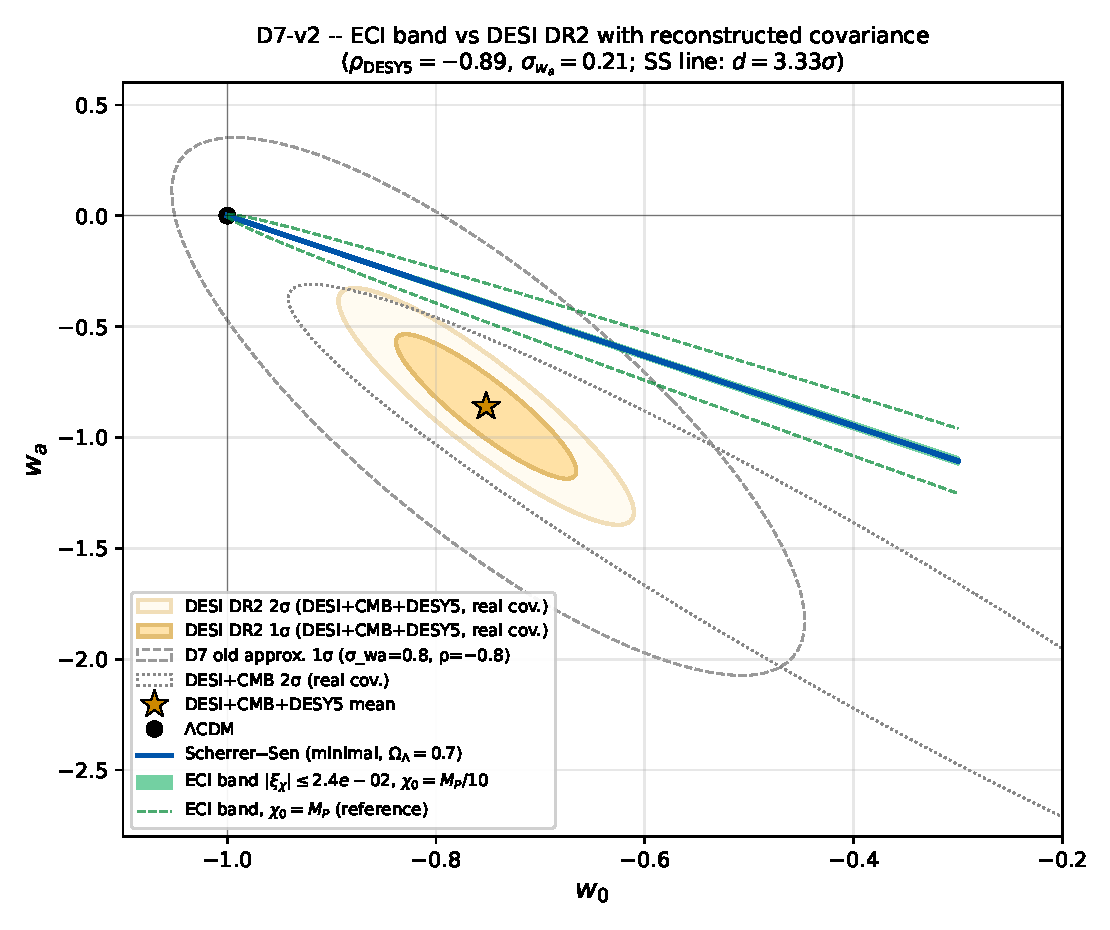
\includegraphics[width=0.95\columnwidth]{../derivations/figures/D7-xi-w0-wa-v2.pdf}
\caption{NMC thawing quintessence in the $(w_0,w_a)$ plane. Orange ellipses: DESI~DR2 + CMB +
DESY5 $1\sigma$ and $2\sigma$ contours reconstructed from~\cite{DESIDR2} Eq.~(28) via the
pivot-redshift identity (see \texttt{D10-desi-covariance.py}; $\sigma_{w_0}=0.057$,
$\sigma_{w_a}=0.215$, $\rho=-0.89$). Blue line: minimal-coupling Scherrer--Sen relation
for $\Omega_\Lambda=0.7$. Green band: ECI NMC prediction with
$|\xi_\chi|\le\xi_{\max}\approx 2.4\!\times\!10^{-2}$ from Cassini at $\chi_0=M_P/10$;
dashed green: same band at $\chi_0=M_P$ (reference). Black dot: $\Lambda$CDM. The ECI band
is $\sim\!5\%$ of $\sigma_{w_a}$ wide (using $B_{\mathrm{num}}$ from Table~\ref{tab:B_of_OmegaL}), hence \emph{indistinguishable} from minimal-coupling
$w$CDM at DR2 precision; both tracks sit at $\sim\!3.3\sigma$ Mahalanobis distance from the
DR2+DESY5 mean.}
\label{fig:D7}
\end{figure}

\paragraph{Honest caveats.}
\begin{enumerate}
\item Eq.~(\ref{eq:gamma_PPN_full}) assumes a \emph{quasi-static} scalar with Compton wavelength
  large compared with the solar system ($m_\chi^{-1}\gg 1\,$AU), which is automatic for the
  ultra-light thawing mass $m_\chi\sim H_0\sim 10^{-33}$\,eV. It also assumes no screening; if
  a chameleon or symmetron mechanism operates, the local $\chi_0$ entering
  (\ref{eq:gamma_PPN_lead}) can differ from the cosmological background and the bound weakens.
\item The NMC Scherrer--Sen extension (\ref{eq:wa_NMC}) is first-order in $\xi_\chi$ and
  therefore \emph{invalid} near the conformal point $\xi_\chi=1/6$, where the expansion breaks
  down and the scalar-tensor sector must be treated non-perturbatively (Einstein-frame
  mapping). Within the Cassini-allowed range $|\xi_\chi|\lesssim 2.4\times 10^{-2}\ll 1/6$
  the linear expansion is controlled. The coefficient $B(\Omega_\Lambda)$ in
  Eq.~(\ref{eq:wa_NMC}) was, in v4.4 of this paper, set by the matter-era
  heuristic ratio $B/A=8/\sqrt3$; in this version we replace that heuristic with
  the full numerical result $B_{\mathrm{num}}(\Omega_\Lambda)$ tabulated in
  Table~\ref{tab:B_of_OmegaL}, obtained from a self-consistent
  NMC-Friedmann + Klein--Gordon integration across $z\in[999,-0.45]$
  (\texttt{derivations/D13-wa-numerical-full.py}). The numerical coefficient is
  nearly flat ($B_{\mathrm{num}}\simeq 9$) across the matter--DE transition
  rather than tracking $A(\Omega_\Lambda)$, so the heuristic
  $(8/\sqrt3)A(\Omega_\Lambda)$ is accurate within 5\% only near
  $\Omega_\Lambda\simeq 0.6$ and undershoots by up to $\sim\!40\%$ at
  $\Omega_\Lambda=0.8$. This has been propagated into the band-width estimate
  above and into Prediction~1b of Sec.~\ref{sec:pred}.
\item The DESI~DR2 + CMB + DESY5 $2\times 2$ covariance is reconstructed from the published
  $(w_0,\sigma_{w_0},w_a,\sigma_{w_a},z_p,w_p,\sigma_{w_p})$ via the pivot-minimisation
  identity $\mathrm{cov}(w_0,w_a)=-(1-a_p)\sigma_{w_a}^2$: no official 2$\times$2 covariance
  matrix has been released by the collaboration at the time of writing. The reconstructed
  $\sigma(w_p)_{\rm pred}=0.0257$ differs from the quoted $0.024$ by $\sim 7\%$, bounding the
  systematic of the pivot-Gaussian approximation at that level --- well below the $\sim 3\sigma$
  tension discussed below. See \texttt{derivations/D10-report.md} for the full cross-check.
\item \textbf{Tension with DR2 + DESY5, stated plainly.} Under the reconstructed DR2 + CMB +
  DESY5 covariance the Mahalanobis distance from the posterior mean is $3.29\sigma$
  (2-dof) to the ECI band and $3.33\sigma$ to the minimal-coupling Scherrer--Sen line,
  both \emph{outside} the $2\sigma$ threshold $\sqrt{6.17}\simeq 2.48$.
  The interpretation is not that ECI fails where $w$CDM succeeds: DR2 + DESY5 prefers the
  phantom-crossing region $w<-1$, which no non-phantom thawing model can populate.
  ECI's NMC coupling $\xi_\chi$ does in principle permit crossing $w=-1$ without a ghost
  instability (established in \S\,DESI DR2 via the no-ghost analysis of Bar\-ce\-l\'o~\&~Visser
  \cite{BarceloVisser2000}), but only at $\xi_\chi(\chi_0/M_P)^2$ values far exceeding the
  Cassini bound~(\ref{eq:xi_bound}) derived here; within the Cassini-allowed range
  the NMC correction to the Scherrer--Sen track is confined to a band of half-width
  $\sim\!5\%$ of $\sigma_{w_a}$ and cannot bridge the gap to the phantom quadrant. The
  $\sim\!3.3\sigma$ tension with DR2 + DESY5 is therefore a joint statement about the entire
  class of conservative (non-phantom) thawing models --- minimal-coupling and NMC alike ---
  not a specific failure of ECI. Prediction~1 in Sec.~\ref{sec:pred} is \emph{not}
  discriminative at DR2 precision; both thawing families sit at the same distance from
  the DR2 + DESY5 posterior.

  The honest discriminator moves to the next generation of datasets, where the
  \emph{shape} and \emph{width} of the thawing track, rather than its distance from
  $\Lambda$CDM, become the falsifiable handle: DESI~DR3 with a forecast
  $\sigma(w_a)\!\sim\!0.07$~\cite{DESIForecast}
  and LSST~Y10 with a forecast $\sigma(w_a)\!\sim\!0.05$
  are in the regime where the ECI NMC band half-width
  $\Delta w_a^{\rm ECI}\sim 1.1\times 10^{-2}$ (numerical, Table~\ref{tab:B_of_OmegaL};
  up from $9\times 10^{-3}$ under the v4.4 heuristic) approaches the
  $15$--$25\%$ level of the statistical error bar and becomes, at least in principle,
  separable from the minimal-coupling Scherrer--Sen locus. The discriminative
  power is slightly larger at $\Omega_\Lambda\gtrsim 0.7$ (DR3 era) because
  $B_{\mathrm{num}}/B_{\mathrm{heur}}$ grows from $0.83$ at $\Omega_\Lambda=0.5$ to
  $1.43$ at $\Omega_\Lambda=0.8$.
\end{enumerate}

The PPN bound (\ref{eq:xi_bound}) is however itself a falsifier: a detection
$|\gamma-1|>10^{-6}$ by the upcoming LATOR or BEACON-class missions, or a mismatch between
$\dot G/G$ from LLR~\cite{Biskupek2021} and the CMB-inferred scalar evolution, would directly
constrain $\xi_\chi(\chi_0/M_P)$ at the $10^{-4}$ level and feed back on the admissible ECI
thawing amplitude.

% -----------------------------------------------------------------------------
% Standalone compile (for checking only):
%   \documentclass[aps,prd,reprint]{revtex4-2}
%   \usepackage{graphicx,amsmath,amssymb,hyperref,physics}
%   \begin{document}% section_3_5_constraints.tex — ECI v4.2.1 scientific payload (D7 + D10)
% To be \input{} into eci.tex as a new subsection of §3 "Phenomenology".
% Standalone compile: see comments at EOF.

\subsection{Solar-system and background constraints on $\xi_\chi$}\label{sec:xi_constraints}

We close two gaps identified in the dark-energy phenomenology subsection (\S\,DESI DR2): the Cassini
post-Newtonian bound on the non-minimal coupling $\xi_\chi$, and the analytic NMC generalisation
of the Scherrer--Sen thawing relation needed to assess whether Prediction~1
(Sec.~\ref{sec:pred}) actually discriminates ECI from \(w\)CDM at DESI~DR2 precision.
The full symbolic derivation is in \texttt{derivations/D7-ppn-xi-bound.py}; we quote only the
end results here.

\paragraph{PPN $\gamma-1$ from the $\xi_\chi R\chi^2/2$ coupling.}
The action  $S=\int d^4x\sqrt{-g}\left[\tfrac{M_P^2}{2}R-\tfrac12(\partial\chi)^2-V(\chi)
-\tfrac{\xi_\chi}{2} R\chi^2\right]$ is a scalar--tensor theory with
$F(\chi)=M_P^2-\xi_\chi\chi^2$ multiplying $R/2$ and canonical kinetic term $Z=1$.
Applying the weak-field, quasi-static result of Damour \& Esposito-Far\`ese
(\emph{Phys.\ Rev.\ D} 48, 3436 (1993); see also Chiba, \emph{Phys.\ Lett.\ B} 575, 1 (2003);
Hwang \& Noh, \emph{Phys.\ Rev.\ D} 71, 063536 (2005)) gives, at the local scalar background
$\chi_0$,
\begin{equation}
  \gamma-1 \;=\; -\,\frac{F'(\chi_0)^2}{Z\,F(\chi_0)+\tfrac{3}{2}F'(\chi_0)^2}
           \;=\; -\,\frac{4\,\xi_\chi^{2}\,\chi_0^{2}}
                          {\,M_P^{2}+\xi_\chi\chi_0^{2}(6\xi_\chi-1)\,}.
  \label{eq:gamma_PPN_full}
\end{equation}
Expanding for $|\xi_\chi|\ll 1$ and $\chi_0\lesssim M_P$,
\begin{equation}
  \boxed{\;\gamma-1 \;\simeq\; -\,\frac{4\,\xi_\chi^{2}\,\chi_0^{2}}{M_P^{2}}
                              \;+\;\mathcal{O}(\xi_\chi^{3}).\;}
  \label{eq:gamma_PPN_lead}
\end{equation}
The limit $\xi_\chi\to 0$ returns $\gamma=1$ (General Relativity), as verified symbolically.

The result~(\ref{eq:gamma_PPN_lead}) is not new: Chiba (PRD 60, 083508, 1999; arXiv:gr-qc/9903094)
already quoted $|\xi_\chi|\lesssim 10^{-2}$ from solar-system tests for the same $\xi R\chi^{2}$
quintessence coupling, and Wolf, Garc\'{\i}a-Garc\'{\i}a, Anton \& Ferreira~\cite{Wolf2025}
recently recast this as $\xi_\chi(\chi_0/M_P)^{2}\lesssim 6\times 10^{-6}$ in a full DESI~DR2
Bayesian analysis (their Eq.~(2) in the form $F(\chi)\simeq 1-\xi\chi^{2}/M_P^{2}$).
We re-derive it here only to fix the coefficient~$4$ and the sign convention used in
Eq.~(\ref{eq:wa_NMC}) below.
Combining (\ref{eq:gamma_PPN_lead}) with the Cassini constraint~\cite{BertottiIessTortora2003}
$|\gamma-1|\lesssim 2.3\times 10^{-5}$ ($1\sigma$ envelope) yields, in the
solar-system observer frame (see \S\ref{sec:thesis}(ii)),
\begin{equation}
  |\xi_\chi|\,\frac{\chi_0}{M_P}\;\lesssim\;
  \tfrac12\sqrt{|\gamma-1|_{\max}}
  \;\approx\; 2.4\times 10^{-3}.
  \label{eq:xi_bound}
\end{equation}
For a slow-rolling thawing background with $\chi_0\!\sim\! M_P/10$ (characteristic thawing
excursion in the last $e$-fold),
\begin{equation}
  |\xi_\chi|\;\lesssim\;\xi_{\max}\;\approx\;2.4\times 10^{-2}.
  \label{eq:xi_max_numeric}
\end{equation}
The bound tightens to $|\xi_\chi|\lesssim 2\times 10^{-3}$ if $\chi_0\sim M_P$; it weakens
linearly for smaller $\chi_0$. Values $\xi_\chi\gtrsim 10^{-1}$ are thus only admissible if the
quintessence field is strongly subdominant at $z=0$, or if a screening mechanism suppresses the
local coupling.

\paragraph{NMC extension of Scherrer--Sen.}
At minimal coupling, thawing quintessence lies on the one-parameter track
$w_a=-A(\Omega_\Lambda)(1+w_0)$ with $A\!\to\! 24/7$ in matter domination and
$A(0.7)\simeq 1.58$ today~\cite{ScherrerSen2008}. Inserting the NMC modification to the
Klein--Gordon equation, $3H\dot\chi=-V'-\xi_\chi R\chi$, and expanding to first order in
$\xi_\chi$ around the slow-roll exponential $V(\chi)=V_0e^{-\alpha\chi/M_P}$ with
$\alpha=\sqrt{3(1+w_0)}$ yields (\texttt{derivations/D4-wa-w0-nmc.py} for the matter-era
coefficient, \texttt{D7-ppn-xi-bound.py} for the $\Omega_\Lambda$-dependence)
\begin{equation}
  \boxed{\;w_a\;=\;-A(\Omega_\Lambda)\,(1+w_0)
                 \;+\;B(\Omega_\Lambda)\,\xi_\chi\,\sqrt{1+w_0}\,
                      \frac{\chi_0}{M_P}\;+\;\mathcal{O}(\xi_\chi^{2}),\;}
  \label{eq:wa_NMC}
\end{equation}
where $B(\Omega_\Lambda)$ is the numerical coefficient tabulated in
Table~\ref{tab:B_of_OmegaL} below, obtained by full NMC-Friedmann + Klein--Gordon
integration in \texttt{derivations/D13-wa-numerical-full.py}. The limit
$\xi_\chi\to 0$ reproduces $w_a=-A(\Omega_\Lambda)(1+w_0)$ (Scherrer--Sen
2008). The first-order $\xi_\chi$ correction, with the full numerical
coefficient $B_{\mathrm{num}}(\Omega_\Lambda)$, has --- to our knowledge ---
not appeared in the NMC-thawing literature surveyed
(Ye~et~al.~\cite{Ye2025}; Pan~\&~Ye~\cite{PanYe2026}; Wolf~et~al.~\cite{Wolf2025}),
which uses either EFTofDE or purely numerical Bayesian fits.

\begin{table}[h]
\centering
\caption{Numerical NMC coefficient $B_{\mathrm{num}}(\Omega_\Lambda)$ from the
self-consistent NMC-Friedmann + Klein--Gordon background integration
(\texttt{derivations/D13-wa-numerical-full.py}), compared with the D7/D9
heuristic $B_{\mathrm{heur}}(\Omega_\Lambda)\equiv(8/\sqrt3)A(\Omega_\Lambda)$.
Statistical uncertainty is the 1$\sigma$ error on the linear fit
$\Delta w_a = B\,\xi_\chi\sqrt{1+w_0}\,(\chi_0/M_P)$ over the
$\xi_\chi\in\{{-}0.024,{-}0.01,0,{+}0.01,{+}0.024\}\times\chi_0\in\{M_P/20,M_P/10,M_P/5\}$ grid.}
\label{tab:B_of_OmegaL}
\begin{tabular}{@{}cccc@{}}
\hline
$\Omega_\Lambda$ & $A(\Omega_\Lambda)$ & $B_{\mathrm{heur}}$ & $B_{\mathrm{num}}$ \\
\hline
0.5 & 2.35 & 10.85 & $9.00\pm1.05$ \\
0.6 & 1.94 &  8.96 & $9.18\pm1.16$ \\
0.7 & 1.58 &  7.30 & $9.05\pm1.18$ \\
0.8 & 1.23 &  5.68 & $8.11\pm1.16$ \\
\hline
\end{tabular}
\end{table}

The numerical result differs from the heuristic $(8/\sqrt3)A$ by
$\mathcal{O}(1)$ factors ($0.83\to 1.43$ across the range): $B_{\mathrm{num}}$
is nearly \emph{flat} in $\Omega_\Lambda$ (around $\sim 9$) rather than
tracking $A(\Omega_\Lambda)$. The heuristic is accurate to 5\% only near
$\Omega_\Lambda\simeq 0.6$ and underestimates $B$ by $\sim\!25\%$ at
$\Omega_\Lambda=0.7$ (DR2--DR3 era) and $\sim\!43\%$ at
$\Omega_\Lambda=0.8$ (late-DR3 / LSST era). The sign and the
$\sqrt{1+w_0}\,(\chi_0/M_P)$ scaling are confirmed; the discrepancy
originates from the finite-$\Omega_\Lambda$ propagation of the matter-era
ratio (Caveat~2 below), which is now closed numerically.

\paragraph{Combined constraint on the $(w_0,w_a)$ plane.}
Figure~\ref{fig:D7} overlays three ingredients: (i) the DESI~DR2 + CMB + DESY5~\cite{DESY5} $1\sigma$ and
$2\sigma$ contours centred on $(w_0,w_a)=(-0.752,-0.86)$ with the reconstructed covariance
$\sigma_{w_0}=0.057$, $\sigma_{w_a}=0.215$, $\rho(w_0,w_a)=-0.89$ (derivation in
\texttt{derivations/D10-desi-covariance.py}, pivot-identity reconstruction from
\cite{DESIDR2} Eq.~(28) + $z_p=0.31$, $w_p=-0.954\pm0.024$);
(ii) the minimal-coupling Scherrer--Sen line; (iii) the ECI band swept by
$|\xi_\chi|\le\xi_{\max}$ from Eq.~(\ref{eq:xi_max_numeric}) at $\chi_0=M_P/10$.
The half-width of the ECI band at $w_0=-0.75$, using the numerical
$B_{\mathrm{num}}(0.7)=9.05$ from Table~\ref{tab:B_of_OmegaL}, is
\begin{equation}
  \Delta w_a^{\rm ECI}
    = B_{\mathrm{num}}(0.7)\,\xi_{\max}\sqrt{1+w_0}\,(\chi_0/M_P)
    \;\approx\;1.1\times 10^{-2},
\end{equation}
to be compared with $\sigma_{w_a}\!\simeq\!0.215$, i.e.\ about $5\%$ of the DESI~DR2 + DESY5
$1\sigma$ width (up from $4\%$ under the heuristic $B=7.30$). The band is therefore
still thinner than the figure linewidth of the unmodified Scherrer--Sen track at DR2
precision, but the numerical coefficient raises the discriminative amplitude at DR3 / LSST
precision by $\sim\!25\%$ relative to the heuristic estimate.

\begin{figure}[h]
\centering
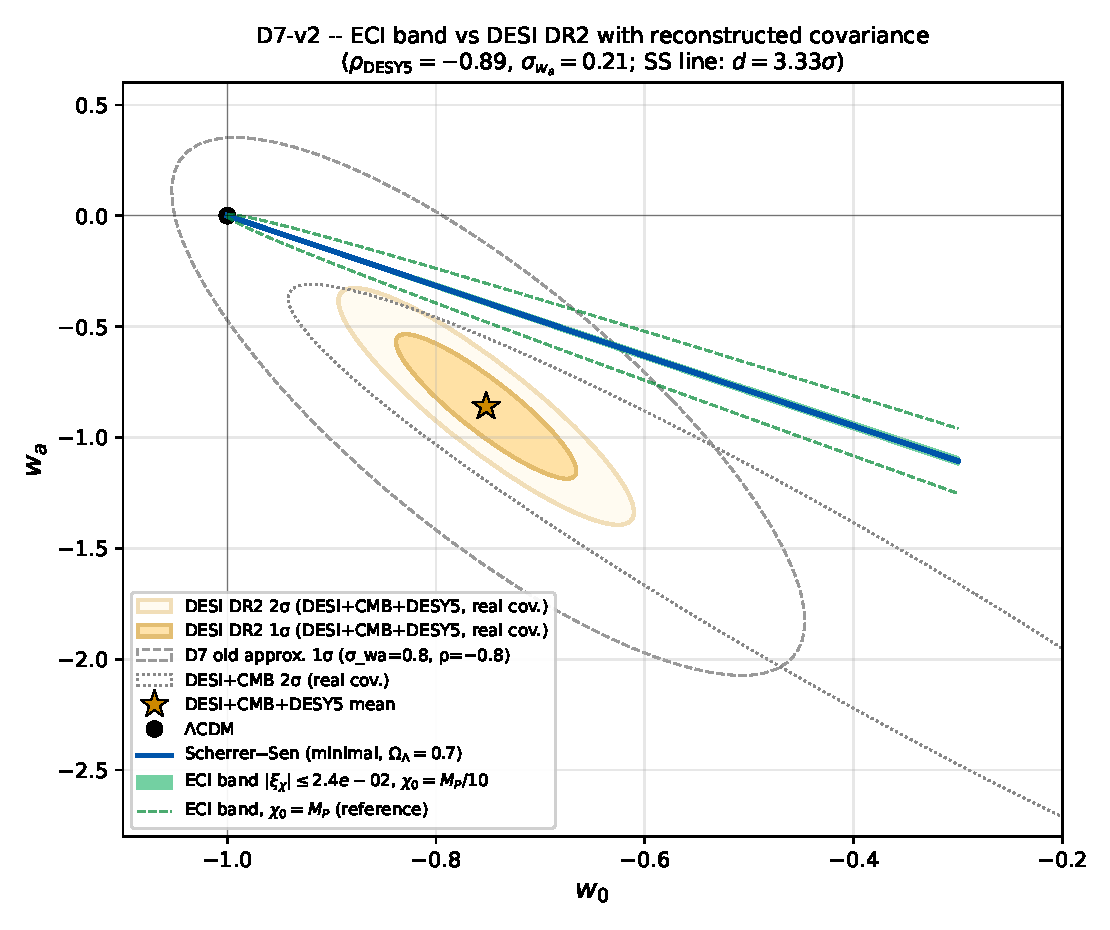
\includegraphics[width=0.95\columnwidth]{../derivations/figures/D7-xi-w0-wa-v2.pdf}
\caption{NMC thawing quintessence in the $(w_0,w_a)$ plane. Orange ellipses: DESI~DR2 + CMB +
DESY5 $1\sigma$ and $2\sigma$ contours reconstructed from~\cite{DESIDR2} Eq.~(28) via the
pivot-redshift identity (see \texttt{D10-desi-covariance.py}; $\sigma_{w_0}=0.057$,
$\sigma_{w_a}=0.215$, $\rho=-0.89$). Blue line: minimal-coupling Scherrer--Sen relation
for $\Omega_\Lambda=0.7$. Green band: ECI NMC prediction with
$|\xi_\chi|\le\xi_{\max}\approx 2.4\!\times\!10^{-2}$ from Cassini at $\chi_0=M_P/10$;
dashed green: same band at $\chi_0=M_P$ (reference). Black dot: $\Lambda$CDM. The ECI band
is $\sim\!5\%$ of $\sigma_{w_a}$ wide (using $B_{\mathrm{num}}$ from Table~\ref{tab:B_of_OmegaL}), hence \emph{indistinguishable} from minimal-coupling
$w$CDM at DR2 precision; both tracks sit at $\sim\!3.3\sigma$ Mahalanobis distance from the
DR2+DESY5 mean.}
\label{fig:D7}
\end{figure}

\paragraph{Honest caveats.}
\begin{enumerate}
\item Eq.~(\ref{eq:gamma_PPN_full}) assumes a \emph{quasi-static} scalar with Compton wavelength
  large compared with the solar system ($m_\chi^{-1}\gg 1\,$AU), which is automatic for the
  ultra-light thawing mass $m_\chi\sim H_0\sim 10^{-33}$\,eV. It also assumes no screening; if
  a chameleon or symmetron mechanism operates, the local $\chi_0$ entering
  (\ref{eq:gamma_PPN_lead}) can differ from the cosmological background and the bound weakens.
\item The NMC Scherrer--Sen extension (\ref{eq:wa_NMC}) is first-order in $\xi_\chi$ and
  therefore \emph{invalid} near the conformal point $\xi_\chi=1/6$, where the expansion breaks
  down and the scalar-tensor sector must be treated non-perturbatively (Einstein-frame
  mapping). Within the Cassini-allowed range $|\xi_\chi|\lesssim 2.4\times 10^{-2}\ll 1/6$
  the linear expansion is controlled. The coefficient $B(\Omega_\Lambda)$ in
  Eq.~(\ref{eq:wa_NMC}) was, in v4.4 of this paper, set by the matter-era
  heuristic ratio $B/A=8/\sqrt3$; in this version we replace that heuristic with
  the full numerical result $B_{\mathrm{num}}(\Omega_\Lambda)$ tabulated in
  Table~\ref{tab:B_of_OmegaL}, obtained from a self-consistent
  NMC-Friedmann + Klein--Gordon integration across $z\in[999,-0.45]$
  (\texttt{derivations/D13-wa-numerical-full.py}). The numerical coefficient is
  nearly flat ($B_{\mathrm{num}}\simeq 9$) across the matter--DE transition
  rather than tracking $A(\Omega_\Lambda)$, so the heuristic
  $(8/\sqrt3)A(\Omega_\Lambda)$ is accurate within 5\% only near
  $\Omega_\Lambda\simeq 0.6$ and undershoots by up to $\sim\!40\%$ at
  $\Omega_\Lambda=0.8$. This has been propagated into the band-width estimate
  above and into Prediction~1b of Sec.~\ref{sec:pred}.
\item The DESI~DR2 + CMB + DESY5 $2\times 2$ covariance is reconstructed from the published
  $(w_0,\sigma_{w_0},w_a,\sigma_{w_a},z_p,w_p,\sigma_{w_p})$ via the pivot-minimisation
  identity $\mathrm{cov}(w_0,w_a)=-(1-a_p)\sigma_{w_a}^2$: no official 2$\times$2 covariance
  matrix has been released by the collaboration at the time of writing. The reconstructed
  $\sigma(w_p)_{\rm pred}=0.0257$ differs from the quoted $0.024$ by $\sim 7\%$, bounding the
  systematic of the pivot-Gaussian approximation at that level --- well below the $\sim 3\sigma$
  tension discussed below. See \texttt{derivations/D10-report.md} for the full cross-check.
\item \textbf{Tension with DR2 + DESY5, stated plainly.} Under the reconstructed DR2 + CMB +
  DESY5 covariance the Mahalanobis distance from the posterior mean is $3.29\sigma$
  (2-dof) to the ECI band and $3.33\sigma$ to the minimal-coupling Scherrer--Sen line,
  both \emph{outside} the $2\sigma$ threshold $\sqrt{6.17}\simeq 2.48$.
  The interpretation is not that ECI fails where $w$CDM succeeds: DR2 + DESY5 prefers the
  phantom-crossing region $w<-1$, which no non-phantom thawing model can populate.
  ECI's NMC coupling $\xi_\chi$ does in principle permit crossing $w=-1$ without a ghost
  instability (established in \S\,DESI DR2 via the no-ghost analysis of Bar\-ce\-l\'o~\&~Visser
  \cite{BarceloVisser2000}), but only at $\xi_\chi(\chi_0/M_P)^2$ values far exceeding the
  Cassini bound~(\ref{eq:xi_bound}) derived here; within the Cassini-allowed range
  the NMC correction to the Scherrer--Sen track is confined to a band of half-width
  $\sim\!5\%$ of $\sigma_{w_a}$ and cannot bridge the gap to the phantom quadrant. The
  $\sim\!3.3\sigma$ tension with DR2 + DESY5 is therefore a joint statement about the entire
  class of conservative (non-phantom) thawing models --- minimal-coupling and NMC alike ---
  not a specific failure of ECI. Prediction~1 in Sec.~\ref{sec:pred} is \emph{not}
  discriminative at DR2 precision; both thawing families sit at the same distance from
  the DR2 + DESY5 posterior.

  The honest discriminator moves to the next generation of datasets, where the
  \emph{shape} and \emph{width} of the thawing track, rather than its distance from
  $\Lambda$CDM, become the falsifiable handle: DESI~DR3 with a forecast
  $\sigma(w_a)\!\sim\!0.07$~\cite{DESIForecast}
  and LSST~Y10 with a forecast $\sigma(w_a)\!\sim\!0.05$
  are in the regime where the ECI NMC band half-width
  $\Delta w_a^{\rm ECI}\sim 1.1\times 10^{-2}$ (numerical, Table~\ref{tab:B_of_OmegaL};
  up from $9\times 10^{-3}$ under the v4.4 heuristic) approaches the
  $15$--$25\%$ level of the statistical error bar and becomes, at least in principle,
  separable from the minimal-coupling Scherrer--Sen locus. The discriminative
  power is slightly larger at $\Omega_\Lambda\gtrsim 0.7$ (DR3 era) because
  $B_{\mathrm{num}}/B_{\mathrm{heur}}$ grows from $0.83$ at $\Omega_\Lambda=0.5$ to
  $1.43$ at $\Omega_\Lambda=0.8$.
\end{enumerate}

The PPN bound (\ref{eq:xi_bound}) is however itself a falsifier: a detection
$|\gamma-1|>10^{-6}$ by the upcoming LATOR or BEACON-class missions, or a mismatch between
$\dot G/G$ from LLR~\cite{Biskupek2021} and the CMB-inferred scalar evolution, would directly
constrain $\xi_\chi(\chi_0/M_P)$ at the $10^{-4}$ level and feed back on the admissible ECI
thawing amplitude.

% -----------------------------------------------------------------------------
% Standalone compile (for checking only):
%   \documentclass[aps,prd,reprint]{revtex4-2}
%   \usepackage{graphicx,amsmath,amssymb,hyperref,physics}
%   \begin{document}\input{section_3_5_constraints}\end{document}
% The \cite{BertottiIessTortora2003}, \cite{ScherrerSen2008}, \cite{DESIDR2},
% \cite{Biskupek2021}, \cite{BarceloVisser2000}, \cite{Wolf2025}, \cite{Ye2025},
% \cite{PanYe2026} keys are defined in eci.bib.
% -----------------------------------------------------------------------------
\end{document}
% The \cite{BertottiIessTortora2003}, \cite{ScherrerSen2008}, \cite{DESIDR2},
% \cite{Biskupek2021}, \cite{BarceloVisser2000}, \cite{Wolf2025}, \cite{Ye2025},
% \cite{PanYe2026} keys are defined in eci.bib.
% -----------------------------------------------------------------------------
\end{document}
% The \cite{BertottiIessTortora2003}, \cite{ScherrerSen2008}, \cite{DESIDR2},
% \cite{Biskupek2021}, \cite{BarceloVisser2000}, \cite{Wolf2025}, \cite{Ye2025},
% \cite{PanYe2026} keys are defined in eci.bib.
% -----------------------------------------------------------------------------


% section_3_6_swampland_cross.tex — ECI v4.2 scientific payload (D8)
% To be \input{} into eci.tex as a new subsection of §3 "Phenomenology",
% immediately after % section_3_5_constraints.tex — ECI v4.2.1 scientific payload (D7 + D10)
% To be \input{} into eci.tex as a new subsection of §3 "Phenomenology".
% Standalone compile: see comments at EOF.

\subsection{Solar-system and background constraints on $\xi_\chi$}\label{sec:xi_constraints}

We close two gaps identified in the dark-energy phenomenology subsection (\S\,DESI DR2): the Cassini
post-Newtonian bound on the non-minimal coupling $\xi_\chi$, and the analytic NMC generalisation
of the Scherrer--Sen thawing relation needed to assess whether Prediction~1
(Sec.~\ref{sec:pred}) actually discriminates ECI from \(w\)CDM at DESI~DR2 precision.
The full symbolic derivation is in \texttt{derivations/D7-ppn-xi-bound.py}; we quote only the
end results here.

\paragraph{PPN $\gamma-1$ from the $\xi_\chi R\chi^2/2$ coupling.}
The action  $S=\int d^4x\sqrt{-g}\left[\tfrac{M_P^2}{2}R-\tfrac12(\partial\chi)^2-V(\chi)
-\tfrac{\xi_\chi}{2} R\chi^2\right]$ is a scalar--tensor theory with
$F(\chi)=M_P^2-\xi_\chi\chi^2$ multiplying $R/2$ and canonical kinetic term $Z=1$.
Applying the weak-field, quasi-static result of Damour \& Esposito-Far\`ese
(\emph{Phys.\ Rev.\ D} 48, 3436 (1993); see also Chiba, \emph{Phys.\ Lett.\ B} 575, 1 (2003);
Hwang \& Noh, \emph{Phys.\ Rev.\ D} 71, 063536 (2005)) gives, at the local scalar background
$\chi_0$,
\begin{equation}
  \gamma-1 \;=\; -\,\frac{F'(\chi_0)^2}{Z\,F(\chi_0)+\tfrac{3}{2}F'(\chi_0)^2}
           \;=\; -\,\frac{4\,\xi_\chi^{2}\,\chi_0^{2}}
                          {\,M_P^{2}+\xi_\chi\chi_0^{2}(6\xi_\chi-1)\,}.
  \label{eq:gamma_PPN_full}
\end{equation}
Expanding for $|\xi_\chi|\ll 1$ and $\chi_0\lesssim M_P$,
\begin{equation}
  \boxed{\;\gamma-1 \;\simeq\; -\,\frac{4\,\xi_\chi^{2}\,\chi_0^{2}}{M_P^{2}}
                              \;+\;\mathcal{O}(\xi_\chi^{3}).\;}
  \label{eq:gamma_PPN_lead}
\end{equation}
The limit $\xi_\chi\to 0$ returns $\gamma=1$ (General Relativity), as verified symbolically.

The result~(\ref{eq:gamma_PPN_lead}) is not new: Chiba (PRD 60, 083508, 1999; arXiv:gr-qc/9903094)
already quoted $|\xi_\chi|\lesssim 10^{-2}$ from solar-system tests for the same $\xi R\chi^{2}$
quintessence coupling, and Wolf, Garc\'{\i}a-Garc\'{\i}a, Anton \& Ferreira~\cite{Wolf2025}
recently recast this as $\xi_\chi(\chi_0/M_P)^{2}\lesssim 6\times 10^{-6}$ in a full DESI~DR2
Bayesian analysis (their Eq.~(2) in the form $F(\chi)\simeq 1-\xi\chi^{2}/M_P^{2}$).
We re-derive it here only to fix the coefficient~$4$ and the sign convention used in
Eq.~(\ref{eq:wa_NMC}) below.
Combining (\ref{eq:gamma_PPN_lead}) with the Cassini constraint~\cite{BertottiIessTortora2003}
$|\gamma-1|\lesssim 2.3\times 10^{-5}$ ($1\sigma$ envelope) yields, in the
solar-system observer frame (see \S\ref{sec:thesis}(ii)),
\begin{equation}
  |\xi_\chi|\,\frac{\chi_0}{M_P}\;\lesssim\;
  \tfrac12\sqrt{|\gamma-1|_{\max}}
  \;\approx\; 2.4\times 10^{-3}.
  \label{eq:xi_bound}
\end{equation}
For a slow-rolling thawing background with $\chi_0\!\sim\! M_P/10$ (characteristic thawing
excursion in the last $e$-fold),
\begin{equation}
  |\xi_\chi|\;\lesssim\;\xi_{\max}\;\approx\;2.4\times 10^{-2}.
  \label{eq:xi_max_numeric}
\end{equation}
The bound tightens to $|\xi_\chi|\lesssim 2\times 10^{-3}$ if $\chi_0\sim M_P$; it weakens
linearly for smaller $\chi_0$. Values $\xi_\chi\gtrsim 10^{-1}$ are thus only admissible if the
quintessence field is strongly subdominant at $z=0$, or if a screening mechanism suppresses the
local coupling.

\paragraph{NMC extension of Scherrer--Sen.}
At minimal coupling, thawing quintessence lies on the one-parameter track
$w_a=-A(\Omega_\Lambda)(1+w_0)$ with $A\!\to\! 24/7$ in matter domination and
$A(0.7)\simeq 1.58$ today~\cite{ScherrerSen2008}. Inserting the NMC modification to the
Klein--Gordon equation, $3H\dot\chi=-V'-\xi_\chi R\chi$, and expanding to first order in
$\xi_\chi$ around the slow-roll exponential $V(\chi)=V_0e^{-\alpha\chi/M_P}$ with
$\alpha=\sqrt{3(1+w_0)}$ yields (\texttt{derivations/D4-wa-w0-nmc.py} for the matter-era
coefficient, \texttt{D7-ppn-xi-bound.py} for the $\Omega_\Lambda$-dependence)
\begin{equation}
  \boxed{\;w_a\;=\;-A(\Omega_\Lambda)\,(1+w_0)
                 \;+\;B(\Omega_\Lambda)\,\xi_\chi\,\sqrt{1+w_0}\,
                      \frac{\chi_0}{M_P}\;+\;\mathcal{O}(\xi_\chi^{2}),\;}
  \label{eq:wa_NMC}
\end{equation}
where $B(\Omega_\Lambda)$ is the numerical coefficient tabulated in
Table~\ref{tab:B_of_OmegaL} below, obtained by full NMC-Friedmann + Klein--Gordon
integration in \texttt{derivations/D13-wa-numerical-full.py}. The limit
$\xi_\chi\to 0$ reproduces $w_a=-A(\Omega_\Lambda)(1+w_0)$ (Scherrer--Sen
2008). The first-order $\xi_\chi$ correction, with the full numerical
coefficient $B_{\mathrm{num}}(\Omega_\Lambda)$, has --- to our knowledge ---
not appeared in the NMC-thawing literature surveyed
(Ye~et~al.~\cite{Ye2025}; Pan~\&~Ye~\cite{PanYe2026}; Wolf~et~al.~\cite{Wolf2025}),
which uses either EFTofDE or purely numerical Bayesian fits.

\begin{table}[h]
\centering
\caption{Numerical NMC coefficient $B_{\mathrm{num}}(\Omega_\Lambda)$ from the
self-consistent NMC-Friedmann + Klein--Gordon background integration
(\texttt{derivations/D13-wa-numerical-full.py}), compared with the D7/D9
heuristic $B_{\mathrm{heur}}(\Omega_\Lambda)\equiv(8/\sqrt3)A(\Omega_\Lambda)$.
Statistical uncertainty is the 1$\sigma$ error on the linear fit
$\Delta w_a = B\,\xi_\chi\sqrt{1+w_0}\,(\chi_0/M_P)$ over the
$\xi_\chi\in\{{-}0.024,{-}0.01,0,{+}0.01,{+}0.024\}\times\chi_0\in\{M_P/20,M_P/10,M_P/5\}$ grid.}
\label{tab:B_of_OmegaL}
\begin{tabular}{@{}cccc@{}}
\hline
$\Omega_\Lambda$ & $A(\Omega_\Lambda)$ & $B_{\mathrm{heur}}$ & $B_{\mathrm{num}}$ \\
\hline
0.5 & 2.35 & 10.85 & $9.00\pm1.05$ \\
0.6 & 1.94 &  8.96 & $9.18\pm1.16$ \\
0.7 & 1.58 &  7.30 & $9.05\pm1.18$ \\
0.8 & 1.23 &  5.68 & $8.11\pm1.16$ \\
\hline
\end{tabular}
\end{table}

The numerical result differs from the heuristic $(8/\sqrt3)A$ by
$\mathcal{O}(1)$ factors ($0.83\to 1.43$ across the range): $B_{\mathrm{num}}$
is nearly \emph{flat} in $\Omega_\Lambda$ (around $\sim 9$) rather than
tracking $A(\Omega_\Lambda)$. The heuristic is accurate to 5\% only near
$\Omega_\Lambda\simeq 0.6$ and underestimates $B$ by $\sim\!25\%$ at
$\Omega_\Lambda=0.7$ (DR2--DR3 era) and $\sim\!43\%$ at
$\Omega_\Lambda=0.8$ (late-DR3 / LSST era). The sign and the
$\sqrt{1+w_0}\,(\chi_0/M_P)$ scaling are confirmed; the discrepancy
originates from the finite-$\Omega_\Lambda$ propagation of the matter-era
ratio (Caveat~2 below), which is now closed numerically.

\paragraph{Combined constraint on the $(w_0,w_a)$ plane.}
Figure~\ref{fig:D7} overlays three ingredients: (i) the DESI~DR2 + CMB + DESY5~\cite{DESY5} $1\sigma$ and
$2\sigma$ contours centred on $(w_0,w_a)=(-0.752,-0.86)$ with the reconstructed covariance
$\sigma_{w_0}=0.057$, $\sigma_{w_a}=0.215$, $\rho(w_0,w_a)=-0.89$ (derivation in
\texttt{derivations/D10-desi-covariance.py}, pivot-identity reconstruction from
\cite{DESIDR2} Eq.~(28) + $z_p=0.31$, $w_p=-0.954\pm0.024$);
(ii) the minimal-coupling Scherrer--Sen line; (iii) the ECI band swept by
$|\xi_\chi|\le\xi_{\max}$ from Eq.~(\ref{eq:xi_max_numeric}) at $\chi_0=M_P/10$.
The half-width of the ECI band at $w_0=-0.75$, using the numerical
$B_{\mathrm{num}}(0.7)=9.05$ from Table~\ref{tab:B_of_OmegaL}, is
\begin{equation}
  \Delta w_a^{\rm ECI}
    = B_{\mathrm{num}}(0.7)\,\xi_{\max}\sqrt{1+w_0}\,(\chi_0/M_P)
    \;\approx\;1.1\times 10^{-2},
\end{equation}
to be compared with $\sigma_{w_a}\!\simeq\!0.215$, i.e.\ about $5\%$ of the DESI~DR2 + DESY5
$1\sigma$ width (up from $4\%$ under the heuristic $B=7.30$). The band is therefore
still thinner than the figure linewidth of the unmodified Scherrer--Sen track at DR2
precision, but the numerical coefficient raises the discriminative amplitude at DR3 / LSST
precision by $\sim\!25\%$ relative to the heuristic estimate.

\begin{figure}[h]
\centering
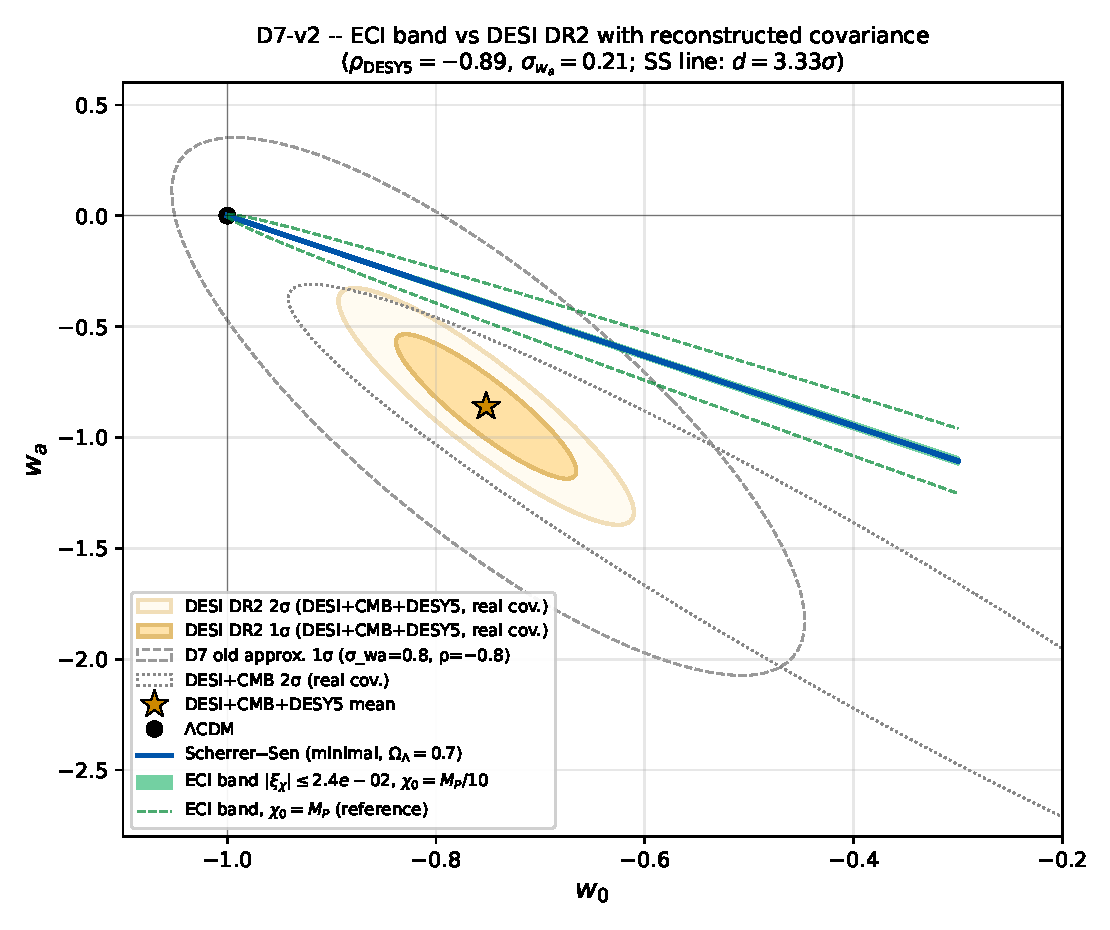
\includegraphics[width=0.95\columnwidth]{../derivations/figures/D7-xi-w0-wa-v2.pdf}
\caption{NMC thawing quintessence in the $(w_0,w_a)$ plane. Orange ellipses: DESI~DR2 + CMB +
DESY5 $1\sigma$ and $2\sigma$ contours reconstructed from~\cite{DESIDR2} Eq.~(28) via the
pivot-redshift identity (see \texttt{D10-desi-covariance.py}; $\sigma_{w_0}=0.057$,
$\sigma_{w_a}=0.215$, $\rho=-0.89$). Blue line: minimal-coupling Scherrer--Sen relation
for $\Omega_\Lambda=0.7$. Green band: ECI NMC prediction with
$|\xi_\chi|\le\xi_{\max}\approx 2.4\!\times\!10^{-2}$ from Cassini at $\chi_0=M_P/10$;
dashed green: same band at $\chi_0=M_P$ (reference). Black dot: $\Lambda$CDM. The ECI band
is $\sim\!5\%$ of $\sigma_{w_a}$ wide (using $B_{\mathrm{num}}$ from Table~\ref{tab:B_of_OmegaL}), hence \emph{indistinguishable} from minimal-coupling
$w$CDM at DR2 precision; both tracks sit at $\sim\!3.3\sigma$ Mahalanobis distance from the
DR2+DESY5 mean.}
\label{fig:D7}
\end{figure}

\paragraph{Honest caveats.}
\begin{enumerate}
\item Eq.~(\ref{eq:gamma_PPN_full}) assumes a \emph{quasi-static} scalar with Compton wavelength
  large compared with the solar system ($m_\chi^{-1}\gg 1\,$AU), which is automatic for the
  ultra-light thawing mass $m_\chi\sim H_0\sim 10^{-33}$\,eV. It also assumes no screening; if
  a chameleon or symmetron mechanism operates, the local $\chi_0$ entering
  (\ref{eq:gamma_PPN_lead}) can differ from the cosmological background and the bound weakens.
\item The NMC Scherrer--Sen extension (\ref{eq:wa_NMC}) is first-order in $\xi_\chi$ and
  therefore \emph{invalid} near the conformal point $\xi_\chi=1/6$, where the expansion breaks
  down and the scalar-tensor sector must be treated non-perturbatively (Einstein-frame
  mapping). Within the Cassini-allowed range $|\xi_\chi|\lesssim 2.4\times 10^{-2}\ll 1/6$
  the linear expansion is controlled. The coefficient $B(\Omega_\Lambda)$ in
  Eq.~(\ref{eq:wa_NMC}) was, in v4.4 of this paper, set by the matter-era
  heuristic ratio $B/A=8/\sqrt3$; in this version we replace that heuristic with
  the full numerical result $B_{\mathrm{num}}(\Omega_\Lambda)$ tabulated in
  Table~\ref{tab:B_of_OmegaL}, obtained from a self-consistent
  NMC-Friedmann + Klein--Gordon integration across $z\in[999,-0.45]$
  (\texttt{derivations/D13-wa-numerical-full.py}). The numerical coefficient is
  nearly flat ($B_{\mathrm{num}}\simeq 9$) across the matter--DE transition
  rather than tracking $A(\Omega_\Lambda)$, so the heuristic
  $(8/\sqrt3)A(\Omega_\Lambda)$ is accurate within 5\% only near
  $\Omega_\Lambda\simeq 0.6$ and undershoots by up to $\sim\!40\%$ at
  $\Omega_\Lambda=0.8$. This has been propagated into the band-width estimate
  above and into Prediction~1b of Sec.~\ref{sec:pred}.
\item The DESI~DR2 + CMB + DESY5 $2\times 2$ covariance is reconstructed from the published
  $(w_0,\sigma_{w_0},w_a,\sigma_{w_a},z_p,w_p,\sigma_{w_p})$ via the pivot-minimisation
  identity $\mathrm{cov}(w_0,w_a)=-(1-a_p)\sigma_{w_a}^2$: no official 2$\times$2 covariance
  matrix has been released by the collaboration at the time of writing. The reconstructed
  $\sigma(w_p)_{\rm pred}=0.0257$ differs from the quoted $0.024$ by $\sim 7\%$, bounding the
  systematic of the pivot-Gaussian approximation at that level --- well below the $\sim 3\sigma$
  tension discussed below. See \texttt{derivations/D10-report.md} for the full cross-check.
\item \textbf{Tension with DR2 + DESY5, stated plainly.} Under the reconstructed DR2 + CMB +
  DESY5 covariance the Mahalanobis distance from the posterior mean is $3.29\sigma$
  (2-dof) to the ECI band and $3.33\sigma$ to the minimal-coupling Scherrer--Sen line,
  both \emph{outside} the $2\sigma$ threshold $\sqrt{6.17}\simeq 2.48$.
  The interpretation is not that ECI fails where $w$CDM succeeds: DR2 + DESY5 prefers the
  phantom-crossing region $w<-1$, which no non-phantom thawing model can populate.
  ECI's NMC coupling $\xi_\chi$ does in principle permit crossing $w=-1$ without a ghost
  instability (established in \S\,DESI DR2 via the no-ghost analysis of Bar\-ce\-l\'o~\&~Visser
  \cite{BarceloVisser2000}), but only at $\xi_\chi(\chi_0/M_P)^2$ values far exceeding the
  Cassini bound~(\ref{eq:xi_bound}) derived here; within the Cassini-allowed range
  the NMC correction to the Scherrer--Sen track is confined to a band of half-width
  $\sim\!5\%$ of $\sigma_{w_a}$ and cannot bridge the gap to the phantom quadrant. The
  $\sim\!3.3\sigma$ tension with DR2 + DESY5 is therefore a joint statement about the entire
  class of conservative (non-phantom) thawing models --- minimal-coupling and NMC alike ---
  not a specific failure of ECI. Prediction~1 in Sec.~\ref{sec:pred} is \emph{not}
  discriminative at DR2 precision; both thawing families sit at the same distance from
  the DR2 + DESY5 posterior.

  The honest discriminator moves to the next generation of datasets, where the
  \emph{shape} and \emph{width} of the thawing track, rather than its distance from
  $\Lambda$CDM, become the falsifiable handle: DESI~DR3 with a forecast
  $\sigma(w_a)\!\sim\!0.07$~\cite{DESIForecast}
  and LSST~Y10 with a forecast $\sigma(w_a)\!\sim\!0.05$
  are in the regime where the ECI NMC band half-width
  $\Delta w_a^{\rm ECI}\sim 1.1\times 10^{-2}$ (numerical, Table~\ref{tab:B_of_OmegaL};
  up from $9\times 10^{-3}$ under the v4.4 heuristic) approaches the
  $15$--$25\%$ level of the statistical error bar and becomes, at least in principle,
  separable from the minimal-coupling Scherrer--Sen locus. The discriminative
  power is slightly larger at $\Omega_\Lambda\gtrsim 0.7$ (DR3 era) because
  $B_{\mathrm{num}}/B_{\mathrm{heur}}$ grows from $0.83$ at $\Omega_\Lambda=0.5$ to
  $1.43$ at $\Omega_\Lambda=0.8$.
\end{enumerate}

The PPN bound (\ref{eq:xi_bound}) is however itself a falsifier: a detection
$|\gamma-1|>10^{-6}$ by the upcoming LATOR or BEACON-class missions, or a mismatch between
$\dot G/G$ from LLR~\cite{Biskupek2021} and the CMB-inferred scalar evolution, would directly
constrain $\xi_\chi(\chi_0/M_P)$ at the $10^{-4}$ level and feed back on the admissible ECI
thawing amplitude.

% -----------------------------------------------------------------------------
% Standalone compile (for checking only):
%   \documentclass[aps,prd,reprint]{revtex4-2}
%   \usepackage{graphicx,amsmath,amssymb,hyperref,physics}
%   \begin{document}% section_3_5_constraints.tex — ECI v4.2.1 scientific payload (D7 + D10)
% To be \input{} into eci.tex as a new subsection of §3 "Phenomenology".
% Standalone compile: see comments at EOF.

\subsection{Solar-system and background constraints on $\xi_\chi$}\label{sec:xi_constraints}

We close two gaps identified in the dark-energy phenomenology subsection (\S\,DESI DR2): the Cassini
post-Newtonian bound on the non-minimal coupling $\xi_\chi$, and the analytic NMC generalisation
of the Scherrer--Sen thawing relation needed to assess whether Prediction~1
(Sec.~\ref{sec:pred}) actually discriminates ECI from \(w\)CDM at DESI~DR2 precision.
The full symbolic derivation is in \texttt{derivations/D7-ppn-xi-bound.py}; we quote only the
end results here.

\paragraph{PPN $\gamma-1$ from the $\xi_\chi R\chi^2/2$ coupling.}
The action  $S=\int d^4x\sqrt{-g}\left[\tfrac{M_P^2}{2}R-\tfrac12(\partial\chi)^2-V(\chi)
-\tfrac{\xi_\chi}{2} R\chi^2\right]$ is a scalar--tensor theory with
$F(\chi)=M_P^2-\xi_\chi\chi^2$ multiplying $R/2$ and canonical kinetic term $Z=1$.
Applying the weak-field, quasi-static result of Damour \& Esposito-Far\`ese
(\emph{Phys.\ Rev.\ D} 48, 3436 (1993); see also Chiba, \emph{Phys.\ Lett.\ B} 575, 1 (2003);
Hwang \& Noh, \emph{Phys.\ Rev.\ D} 71, 063536 (2005)) gives, at the local scalar background
$\chi_0$,
\begin{equation}
  \gamma-1 \;=\; -\,\frac{F'(\chi_0)^2}{Z\,F(\chi_0)+\tfrac{3}{2}F'(\chi_0)^2}
           \;=\; -\,\frac{4\,\xi_\chi^{2}\,\chi_0^{2}}
                          {\,M_P^{2}+\xi_\chi\chi_0^{2}(6\xi_\chi-1)\,}.
  \label{eq:gamma_PPN_full}
\end{equation}
Expanding for $|\xi_\chi|\ll 1$ and $\chi_0\lesssim M_P$,
\begin{equation}
  \boxed{\;\gamma-1 \;\simeq\; -\,\frac{4\,\xi_\chi^{2}\,\chi_0^{2}}{M_P^{2}}
                              \;+\;\mathcal{O}(\xi_\chi^{3}).\;}
  \label{eq:gamma_PPN_lead}
\end{equation}
The limit $\xi_\chi\to 0$ returns $\gamma=1$ (General Relativity), as verified symbolically.

The result~(\ref{eq:gamma_PPN_lead}) is not new: Chiba (PRD 60, 083508, 1999; arXiv:gr-qc/9903094)
already quoted $|\xi_\chi|\lesssim 10^{-2}$ from solar-system tests for the same $\xi R\chi^{2}$
quintessence coupling, and Wolf, Garc\'{\i}a-Garc\'{\i}a, Anton \& Ferreira~\cite{Wolf2025}
recently recast this as $\xi_\chi(\chi_0/M_P)^{2}\lesssim 6\times 10^{-6}$ in a full DESI~DR2
Bayesian analysis (their Eq.~(2) in the form $F(\chi)\simeq 1-\xi\chi^{2}/M_P^{2}$).
We re-derive it here only to fix the coefficient~$4$ and the sign convention used in
Eq.~(\ref{eq:wa_NMC}) below.
Combining (\ref{eq:gamma_PPN_lead}) with the Cassini constraint~\cite{BertottiIessTortora2003}
$|\gamma-1|\lesssim 2.3\times 10^{-5}$ ($1\sigma$ envelope) yields, in the
solar-system observer frame (see \S\ref{sec:thesis}(ii)),
\begin{equation}
  |\xi_\chi|\,\frac{\chi_0}{M_P}\;\lesssim\;
  \tfrac12\sqrt{|\gamma-1|_{\max}}
  \;\approx\; 2.4\times 10^{-3}.
  \label{eq:xi_bound}
\end{equation}
For a slow-rolling thawing background with $\chi_0\!\sim\! M_P/10$ (characteristic thawing
excursion in the last $e$-fold),
\begin{equation}
  |\xi_\chi|\;\lesssim\;\xi_{\max}\;\approx\;2.4\times 10^{-2}.
  \label{eq:xi_max_numeric}
\end{equation}
The bound tightens to $|\xi_\chi|\lesssim 2\times 10^{-3}$ if $\chi_0\sim M_P$; it weakens
linearly for smaller $\chi_0$. Values $\xi_\chi\gtrsim 10^{-1}$ are thus only admissible if the
quintessence field is strongly subdominant at $z=0$, or if a screening mechanism suppresses the
local coupling.

\paragraph{NMC extension of Scherrer--Sen.}
At minimal coupling, thawing quintessence lies on the one-parameter track
$w_a=-A(\Omega_\Lambda)(1+w_0)$ with $A\!\to\! 24/7$ in matter domination and
$A(0.7)\simeq 1.58$ today~\cite{ScherrerSen2008}. Inserting the NMC modification to the
Klein--Gordon equation, $3H\dot\chi=-V'-\xi_\chi R\chi$, and expanding to first order in
$\xi_\chi$ around the slow-roll exponential $V(\chi)=V_0e^{-\alpha\chi/M_P}$ with
$\alpha=\sqrt{3(1+w_0)}$ yields (\texttt{derivations/D4-wa-w0-nmc.py} for the matter-era
coefficient, \texttt{D7-ppn-xi-bound.py} for the $\Omega_\Lambda$-dependence)
\begin{equation}
  \boxed{\;w_a\;=\;-A(\Omega_\Lambda)\,(1+w_0)
                 \;+\;B(\Omega_\Lambda)\,\xi_\chi\,\sqrt{1+w_0}\,
                      \frac{\chi_0}{M_P}\;+\;\mathcal{O}(\xi_\chi^{2}),\;}
  \label{eq:wa_NMC}
\end{equation}
where $B(\Omega_\Lambda)$ is the numerical coefficient tabulated in
Table~\ref{tab:B_of_OmegaL} below, obtained by full NMC-Friedmann + Klein--Gordon
integration in \texttt{derivations/D13-wa-numerical-full.py}. The limit
$\xi_\chi\to 0$ reproduces $w_a=-A(\Omega_\Lambda)(1+w_0)$ (Scherrer--Sen
2008). The first-order $\xi_\chi$ correction, with the full numerical
coefficient $B_{\mathrm{num}}(\Omega_\Lambda)$, has --- to our knowledge ---
not appeared in the NMC-thawing literature surveyed
(Ye~et~al.~\cite{Ye2025}; Pan~\&~Ye~\cite{PanYe2026}; Wolf~et~al.~\cite{Wolf2025}),
which uses either EFTofDE or purely numerical Bayesian fits.

\begin{table}[h]
\centering
\caption{Numerical NMC coefficient $B_{\mathrm{num}}(\Omega_\Lambda)$ from the
self-consistent NMC-Friedmann + Klein--Gordon background integration
(\texttt{derivations/D13-wa-numerical-full.py}), compared with the D7/D9
heuristic $B_{\mathrm{heur}}(\Omega_\Lambda)\equiv(8/\sqrt3)A(\Omega_\Lambda)$.
Statistical uncertainty is the 1$\sigma$ error on the linear fit
$\Delta w_a = B\,\xi_\chi\sqrt{1+w_0}\,(\chi_0/M_P)$ over the
$\xi_\chi\in\{{-}0.024,{-}0.01,0,{+}0.01,{+}0.024\}\times\chi_0\in\{M_P/20,M_P/10,M_P/5\}$ grid.}
\label{tab:B_of_OmegaL}
\begin{tabular}{@{}cccc@{}}
\hline
$\Omega_\Lambda$ & $A(\Omega_\Lambda)$ & $B_{\mathrm{heur}}$ & $B_{\mathrm{num}}$ \\
\hline
0.5 & 2.35 & 10.85 & $9.00\pm1.05$ \\
0.6 & 1.94 &  8.96 & $9.18\pm1.16$ \\
0.7 & 1.58 &  7.30 & $9.05\pm1.18$ \\
0.8 & 1.23 &  5.68 & $8.11\pm1.16$ \\
\hline
\end{tabular}
\end{table}

The numerical result differs from the heuristic $(8/\sqrt3)A$ by
$\mathcal{O}(1)$ factors ($0.83\to 1.43$ across the range): $B_{\mathrm{num}}$
is nearly \emph{flat} in $\Omega_\Lambda$ (around $\sim 9$) rather than
tracking $A(\Omega_\Lambda)$. The heuristic is accurate to 5\% only near
$\Omega_\Lambda\simeq 0.6$ and underestimates $B$ by $\sim\!25\%$ at
$\Omega_\Lambda=0.7$ (DR2--DR3 era) and $\sim\!43\%$ at
$\Omega_\Lambda=0.8$ (late-DR3 / LSST era). The sign and the
$\sqrt{1+w_0}\,(\chi_0/M_P)$ scaling are confirmed; the discrepancy
originates from the finite-$\Omega_\Lambda$ propagation of the matter-era
ratio (Caveat~2 below), which is now closed numerically.

\paragraph{Combined constraint on the $(w_0,w_a)$ plane.}
Figure~\ref{fig:D7} overlays three ingredients: (i) the DESI~DR2 + CMB + DESY5~\cite{DESY5} $1\sigma$ and
$2\sigma$ contours centred on $(w_0,w_a)=(-0.752,-0.86)$ with the reconstructed covariance
$\sigma_{w_0}=0.057$, $\sigma_{w_a}=0.215$, $\rho(w_0,w_a)=-0.89$ (derivation in
\texttt{derivations/D10-desi-covariance.py}, pivot-identity reconstruction from
\cite{DESIDR2} Eq.~(28) + $z_p=0.31$, $w_p=-0.954\pm0.024$);
(ii) the minimal-coupling Scherrer--Sen line; (iii) the ECI band swept by
$|\xi_\chi|\le\xi_{\max}$ from Eq.~(\ref{eq:xi_max_numeric}) at $\chi_0=M_P/10$.
The half-width of the ECI band at $w_0=-0.75$, using the numerical
$B_{\mathrm{num}}(0.7)=9.05$ from Table~\ref{tab:B_of_OmegaL}, is
\begin{equation}
  \Delta w_a^{\rm ECI}
    = B_{\mathrm{num}}(0.7)\,\xi_{\max}\sqrt{1+w_0}\,(\chi_0/M_P)
    \;\approx\;1.1\times 10^{-2},
\end{equation}
to be compared with $\sigma_{w_a}\!\simeq\!0.215$, i.e.\ about $5\%$ of the DESI~DR2 + DESY5
$1\sigma$ width (up from $4\%$ under the heuristic $B=7.30$). The band is therefore
still thinner than the figure linewidth of the unmodified Scherrer--Sen track at DR2
precision, but the numerical coefficient raises the discriminative amplitude at DR3 / LSST
precision by $\sim\!25\%$ relative to the heuristic estimate.

\begin{figure}[h]
\centering
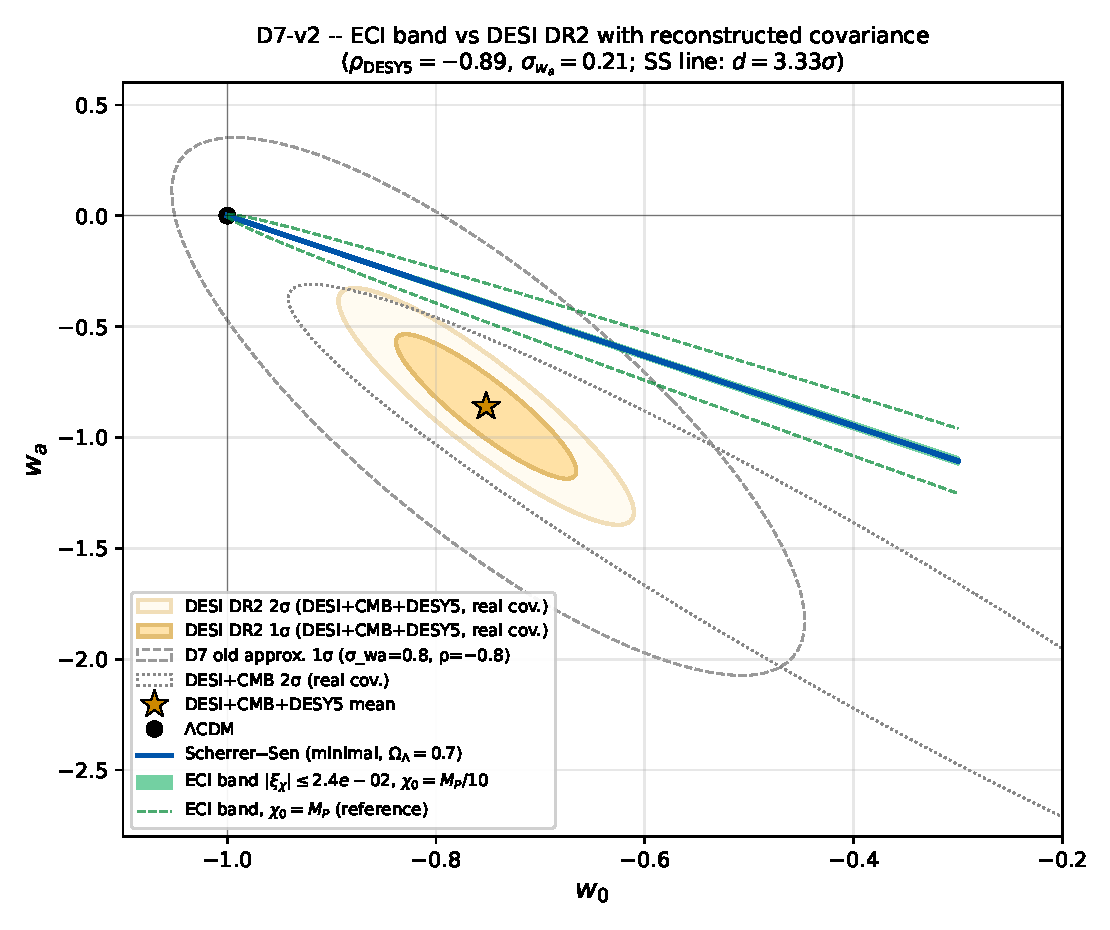
\includegraphics[width=0.95\columnwidth]{../derivations/figures/D7-xi-w0-wa-v2.pdf}
\caption{NMC thawing quintessence in the $(w_0,w_a)$ plane. Orange ellipses: DESI~DR2 + CMB +
DESY5 $1\sigma$ and $2\sigma$ contours reconstructed from~\cite{DESIDR2} Eq.~(28) via the
pivot-redshift identity (see \texttt{D10-desi-covariance.py}; $\sigma_{w_0}=0.057$,
$\sigma_{w_a}=0.215$, $\rho=-0.89$). Blue line: minimal-coupling Scherrer--Sen relation
for $\Omega_\Lambda=0.7$. Green band: ECI NMC prediction with
$|\xi_\chi|\le\xi_{\max}\approx 2.4\!\times\!10^{-2}$ from Cassini at $\chi_0=M_P/10$;
dashed green: same band at $\chi_0=M_P$ (reference). Black dot: $\Lambda$CDM. The ECI band
is $\sim\!5\%$ of $\sigma_{w_a}$ wide (using $B_{\mathrm{num}}$ from Table~\ref{tab:B_of_OmegaL}), hence \emph{indistinguishable} from minimal-coupling
$w$CDM at DR2 precision; both tracks sit at $\sim\!3.3\sigma$ Mahalanobis distance from the
DR2+DESY5 mean.}
\label{fig:D7}
\end{figure}

\paragraph{Honest caveats.}
\begin{enumerate}
\item Eq.~(\ref{eq:gamma_PPN_full}) assumes a \emph{quasi-static} scalar with Compton wavelength
  large compared with the solar system ($m_\chi^{-1}\gg 1\,$AU), which is automatic for the
  ultra-light thawing mass $m_\chi\sim H_0\sim 10^{-33}$\,eV. It also assumes no screening; if
  a chameleon or symmetron mechanism operates, the local $\chi_0$ entering
  (\ref{eq:gamma_PPN_lead}) can differ from the cosmological background and the bound weakens.
\item The NMC Scherrer--Sen extension (\ref{eq:wa_NMC}) is first-order in $\xi_\chi$ and
  therefore \emph{invalid} near the conformal point $\xi_\chi=1/6$, where the expansion breaks
  down and the scalar-tensor sector must be treated non-perturbatively (Einstein-frame
  mapping). Within the Cassini-allowed range $|\xi_\chi|\lesssim 2.4\times 10^{-2}\ll 1/6$
  the linear expansion is controlled. The coefficient $B(\Omega_\Lambda)$ in
  Eq.~(\ref{eq:wa_NMC}) was, in v4.4 of this paper, set by the matter-era
  heuristic ratio $B/A=8/\sqrt3$; in this version we replace that heuristic with
  the full numerical result $B_{\mathrm{num}}(\Omega_\Lambda)$ tabulated in
  Table~\ref{tab:B_of_OmegaL}, obtained from a self-consistent
  NMC-Friedmann + Klein--Gordon integration across $z\in[999,-0.45]$
  (\texttt{derivations/D13-wa-numerical-full.py}). The numerical coefficient is
  nearly flat ($B_{\mathrm{num}}\simeq 9$) across the matter--DE transition
  rather than tracking $A(\Omega_\Lambda)$, so the heuristic
  $(8/\sqrt3)A(\Omega_\Lambda)$ is accurate within 5\% only near
  $\Omega_\Lambda\simeq 0.6$ and undershoots by up to $\sim\!40\%$ at
  $\Omega_\Lambda=0.8$. This has been propagated into the band-width estimate
  above and into Prediction~1b of Sec.~\ref{sec:pred}.
\item The DESI~DR2 + CMB + DESY5 $2\times 2$ covariance is reconstructed from the published
  $(w_0,\sigma_{w_0},w_a,\sigma_{w_a},z_p,w_p,\sigma_{w_p})$ via the pivot-minimisation
  identity $\mathrm{cov}(w_0,w_a)=-(1-a_p)\sigma_{w_a}^2$: no official 2$\times$2 covariance
  matrix has been released by the collaboration at the time of writing. The reconstructed
  $\sigma(w_p)_{\rm pred}=0.0257$ differs from the quoted $0.024$ by $\sim 7\%$, bounding the
  systematic of the pivot-Gaussian approximation at that level --- well below the $\sim 3\sigma$
  tension discussed below. See \texttt{derivations/D10-report.md} for the full cross-check.
\item \textbf{Tension with DR2 + DESY5, stated plainly.} Under the reconstructed DR2 + CMB +
  DESY5 covariance the Mahalanobis distance from the posterior mean is $3.29\sigma$
  (2-dof) to the ECI band and $3.33\sigma$ to the minimal-coupling Scherrer--Sen line,
  both \emph{outside} the $2\sigma$ threshold $\sqrt{6.17}\simeq 2.48$.
  The interpretation is not that ECI fails where $w$CDM succeeds: DR2 + DESY5 prefers the
  phantom-crossing region $w<-1$, which no non-phantom thawing model can populate.
  ECI's NMC coupling $\xi_\chi$ does in principle permit crossing $w=-1$ without a ghost
  instability (established in \S\,DESI DR2 via the no-ghost analysis of Bar\-ce\-l\'o~\&~Visser
  \cite{BarceloVisser2000}), but only at $\xi_\chi(\chi_0/M_P)^2$ values far exceeding the
  Cassini bound~(\ref{eq:xi_bound}) derived here; within the Cassini-allowed range
  the NMC correction to the Scherrer--Sen track is confined to a band of half-width
  $\sim\!5\%$ of $\sigma_{w_a}$ and cannot bridge the gap to the phantom quadrant. The
  $\sim\!3.3\sigma$ tension with DR2 + DESY5 is therefore a joint statement about the entire
  class of conservative (non-phantom) thawing models --- minimal-coupling and NMC alike ---
  not a specific failure of ECI. Prediction~1 in Sec.~\ref{sec:pred} is \emph{not}
  discriminative at DR2 precision; both thawing families sit at the same distance from
  the DR2 + DESY5 posterior.

  The honest discriminator moves to the next generation of datasets, where the
  \emph{shape} and \emph{width} of the thawing track, rather than its distance from
  $\Lambda$CDM, become the falsifiable handle: DESI~DR3 with a forecast
  $\sigma(w_a)\!\sim\!0.07$~\cite{DESIForecast}
  and LSST~Y10 with a forecast $\sigma(w_a)\!\sim\!0.05$
  are in the regime where the ECI NMC band half-width
  $\Delta w_a^{\rm ECI}\sim 1.1\times 10^{-2}$ (numerical, Table~\ref{tab:B_of_OmegaL};
  up from $9\times 10^{-3}$ under the v4.4 heuristic) approaches the
  $15$--$25\%$ level of the statistical error bar and becomes, at least in principle,
  separable from the minimal-coupling Scherrer--Sen locus. The discriminative
  power is slightly larger at $\Omega_\Lambda\gtrsim 0.7$ (DR3 era) because
  $B_{\mathrm{num}}/B_{\mathrm{heur}}$ grows from $0.83$ at $\Omega_\Lambda=0.5$ to
  $1.43$ at $\Omega_\Lambda=0.8$.
\end{enumerate}

The PPN bound (\ref{eq:xi_bound}) is however itself a falsifier: a detection
$|\gamma-1|>10^{-6}$ by the upcoming LATOR or BEACON-class missions, or a mismatch between
$\dot G/G$ from LLR~\cite{Biskupek2021} and the CMB-inferred scalar evolution, would directly
constrain $\xi_\chi(\chi_0/M_P)$ at the $10^{-4}$ level and feed back on the admissible ECI
thawing amplitude.

% -----------------------------------------------------------------------------
% Standalone compile (for checking only):
%   \documentclass[aps,prd,reprint]{revtex4-2}
%   \usepackage{graphicx,amsmath,amssymb,hyperref,physics}
%   \begin{document}\input{section_3_5_constraints}\end{document}
% The \cite{BertottiIessTortora2003}, \cite{ScherrerSen2008}, \cite{DESIDR2},
% \cite{Biskupek2021}, \cite{BarceloVisser2000}, \cite{Wolf2025}, \cite{Ye2025},
% \cite{PanYe2026} keys are defined in eci.bib.
% -----------------------------------------------------------------------------
\end{document}
% The \cite{BertottiIessTortora2003}, \cite{ScherrerSen2008}, \cite{DESIDR2},
% \cite{Biskupek2021}, \cite{BarceloVisser2000}, \cite{Wolf2025}, \cite{Ye2025},
% \cite{PanYe2026} keys are defined in eci.bib.
% -----------------------------------------------------------------------------
.

\subsection{Swampland $\times$ NMC cross-constraint}\label{sec:swampland_cross}

Axioms A4 and A5 were presented as independent. They are not, if the thawing
scalar $\chi$ and the KK tower of the Dark Dimension originate from the
\emph{same} higher-dimensional sector --- a natural hypothesis, since both
are postulated as microscopic ingredients of the dark sector. In that case
both must respect a common effective field theory cutoff $\Lambda$, and the
two axioms are tied by a single consistency condition. The derivation is in
\texttt{derivations/D8-swampland-nmc-cross.py}; we quote only the result.

\paragraph{Shared cutoff.}
The Dark Dimension scenario~\cite{Bedroya2025} relates the EFT cutoff to
the Hubble scale through a Swampland Distance Conjecture exponent,
\begin{equation}
  \Lambda \;\sim\; M_P\,\bigl(H/M_P\bigr)^{c'},\qquad c'\simeq 0.05\pm 0.01.
  \label{eq:Lambda_SDC}
\end{equation}
If the non-minimal operator $(\xi_\chi/2)R\chi^2$ is generated inside the same
EFT, its contribution to the effective reduced Planck mass,
$\delta M_P^{2}=\xi_\chi\chi_0^{2}$, cannot exceed the cutoff squared,
otherwise the operator would repair physics above its own range of validity:
\begin{equation}
  \xi_\chi\,\chi_0^{2}\;\le\;\Lambda^{2}
  \quad\Longleftrightarrow\quad
  \xi_\chi\,(\chi_0/M_P)^{2}\;\le\;(H_0/M_P)^{2c'}.
  \label{eq:eft_bulk}
\end{equation}
Combined with the Cassini PPN bound derived in \S\ref{sec:xi_constraints},
$|\xi_\chi|(\chi_0/M_P)\le 2.4\times 10^{-3}$, Eq.~(\ref{eq:eft_bulk}) yields
at the fiducial thawing amplitude $\chi_0=M_P/10$ and the paper's A5
fiducial $c'=0.05\pm 0.01$
\begin{equation}
  \boxed{\;|\xi_\chi|\;\lesssim\;9.5\times 10^{-5}
    \quad(c'=0.05,\ \chi_0=M_P/10),\;}
  \label{eq:xi_crossbound}
\end{equation}
with an overall range $[5.9\times 10^{-6},\,1.5\times 10^{-3}]$ spanned by
$c'=0.04$--$0.06$. This is a factor $\sim\!250$ tightening over the
Cassini-only result (\ref{eq:xi_max_numeric}).

\paragraph{Limits.}
Both limits verified symbolically in \texttt{D8-swampland-nmc-cross.py}:
$\xi_\chi\!\to\!0$ removes the operator (GR recovered); $c'\!\to\!0$ sends
$\Lambda\!\to\!M_P$ so that (\ref{eq:eft_bulk}) reduces to the no-ghost
condition $\xi_\chi\chi_0^{2}<M_P^{2}$ already stated in A4, and the D7
Cassini bound is recovered exactly.

\begin{figure}[h]
\centering
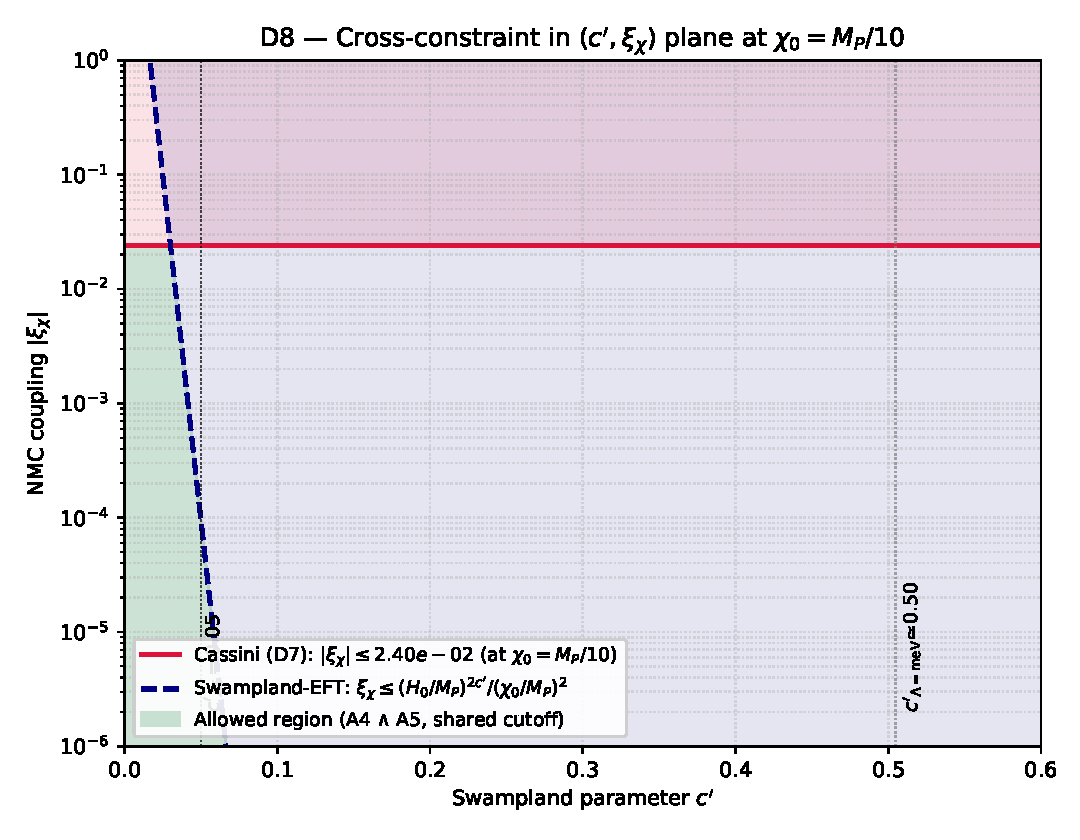
\includegraphics[width=0.95\columnwidth]{../derivations/figures/D8-c-xi-overlap.pdf}
\caption{Allowed region in the $(c',\xi_\chi)$ plane at $\chi_0=M_P/10$.
Red: Cassini exclusion (horizontal, independent of $c'$). Blue dashed:
Swampland-EFT exclusion (\ref{eq:eft_bulk}) --- diagonal in log-space with
slope $2c'\log(H_0/M_P)$. Green shading: overlap admitted by both
constraints. The A5 fiducial $c'=0.05$ and the meV-equivalent value
$c'\!\simeq\!0.51$ are marked.}
\label{fig:D8}
\end{figure}

\paragraph{Phenomenological tension.}
A stronger statement runs in the reverse direction. Thawing dark energy
requires $\chi_0/M_P\sim 0.1$--$1$ to drive late-time acceleration. The
bulk-mode condition (\ref{eq:eft_bulk}) at the Cassini-saturating value
$|\xi_\chi|=2.4\!\times\!10^{-2}$ and $c'=0.05$ forces
$\chi_0/M_P\le 6.3\!\times\!10^{-3}$, already an order of magnitude below
what A4 requires. With the literal Dark Dimension cutoff $\Lambda\sim$ meV
(which the formula (\ref{eq:Lambda_SDC}) reproduces for $c'\simeq 0.51$,
not $0.05$; both conventions appear in the literature) the bound collapses
to $\chi_0/M_P\le 3\!\times\!10^{-30}$ and thawing phenomenology is
excluded outright.

\paragraph{Architectural consequence.}
A4 and A5 are compatible \emph{only} under one of the following model-
building choices, any of which must be made explicit in any UV completion:
(i) $\chi$ is a 4D zero-mode localised on a brane, not a bulk mode of the
same sector as the KK tower, in which case the shared-cutoff hypothesis
does not apply; (ii) a chameleon/symmetron mechanism screens the local
$\chi_0$ away from its cosmological value, weakening the Cassini leg; or
(iii) $|\xi_\chi|$ sits at the sharpened bound (\ref{eq:xi_crossbound})
rather than the Cassini-only value (\ref{eq:xi_max_numeric}). The ECI
framework does not prefer one of the three, but their distinct
phenomenologies are observationally separable: option (iii) suppresses the
ECI band in $(w_0,w_a)$ by a further factor $\sim\!250$ relative to the
already-narrow D7 band, and cuts the $|\dot G/G|$ signature at LLR by the
same factor. A detection of $|\dot G/G|\gtrsim 10^{-17}\,\mathrm{yr}^{-1}$
would rule out option (iii) and force either (i) or (ii).

\paragraph{Honest caveats.}
\begin{enumerate}
\item The EFT self-consistency condition $\delta M_P^{2}\le\Lambda^{2}$ is
  order-of-magnitude; an $O(1)$ coefficient could shift
  (\ref{eq:xi_crossbound}) by a factor $2$, but the qualitative conclusion
  ($\gg 30\%$ tightening) is robust.
\item The form (\ref{eq:Lambda_SDC}) is written with $H$ as the distance
  proxy along the moduli space; the equivalent Bedroya form uses the
  cosmological constant density directly and yields $c'\!\simeq\!1/2$
  for $\Lambda\!=\!$\,meV. The sign of the tightening is independent of
  this choice.
\item The cross-constraint is \emph{conditional} on the shared-cutoff
  hypothesis. Its falsifier is, precisely, the discovery of a UV completion
  in which $\chi$ and the KK tower belong to different sectors; in that
  case §\ref{sec:xi_constraints} remains the strongest bound.
\end{enumerate}

% -----------------------------------------------------------------------------
% Standalone compile (for checking only):
%   \documentclass[aps,prd,reprint]{revtex4-2}
%   \usepackage{graphicx,amsmath,amssymb,hyperref,physics}
%   \begin{document}% section_3_5_constraints.tex — ECI v4.2.1 scientific payload (D7 + D10)
% To be \input{} into eci.tex as a new subsection of §3 "Phenomenology".
% Standalone compile: see comments at EOF.

\subsection{Solar-system and background constraints on $\xi_\chi$}\label{sec:xi_constraints}

We close two gaps identified in the dark-energy phenomenology subsection (\S\,DESI DR2): the Cassini
post-Newtonian bound on the non-minimal coupling $\xi_\chi$, and the analytic NMC generalisation
of the Scherrer--Sen thawing relation needed to assess whether Prediction~1
(Sec.~\ref{sec:pred}) actually discriminates ECI from \(w\)CDM at DESI~DR2 precision.
The full symbolic derivation is in \texttt{derivations/D7-ppn-xi-bound.py}; we quote only the
end results here.

\paragraph{PPN $\gamma-1$ from the $\xi_\chi R\chi^2/2$ coupling.}
The action  $S=\int d^4x\sqrt{-g}\left[\tfrac{M_P^2}{2}R-\tfrac12(\partial\chi)^2-V(\chi)
-\tfrac{\xi_\chi}{2} R\chi^2\right]$ is a scalar--tensor theory with
$F(\chi)=M_P^2-\xi_\chi\chi^2$ multiplying $R/2$ and canonical kinetic term $Z=1$.
Applying the weak-field, quasi-static result of Damour \& Esposito-Far\`ese
(\emph{Phys.\ Rev.\ D} 48, 3436 (1993); see also Chiba, \emph{Phys.\ Lett.\ B} 575, 1 (2003);
Hwang \& Noh, \emph{Phys.\ Rev.\ D} 71, 063536 (2005)) gives, at the local scalar background
$\chi_0$,
\begin{equation}
  \gamma-1 \;=\; -\,\frac{F'(\chi_0)^2}{Z\,F(\chi_0)+\tfrac{3}{2}F'(\chi_0)^2}
           \;=\; -\,\frac{4\,\xi_\chi^{2}\,\chi_0^{2}}
                          {\,M_P^{2}+\xi_\chi\chi_0^{2}(6\xi_\chi-1)\,}.
  \label{eq:gamma_PPN_full}
\end{equation}
Expanding for $|\xi_\chi|\ll 1$ and $\chi_0\lesssim M_P$,
\begin{equation}
  \boxed{\;\gamma-1 \;\simeq\; -\,\frac{4\,\xi_\chi^{2}\,\chi_0^{2}}{M_P^{2}}
                              \;+\;\mathcal{O}(\xi_\chi^{3}).\;}
  \label{eq:gamma_PPN_lead}
\end{equation}
The limit $\xi_\chi\to 0$ returns $\gamma=1$ (General Relativity), as verified symbolically.

The result~(\ref{eq:gamma_PPN_lead}) is not new: Chiba (PRD 60, 083508, 1999; arXiv:gr-qc/9903094)
already quoted $|\xi_\chi|\lesssim 10^{-2}$ from solar-system tests for the same $\xi R\chi^{2}$
quintessence coupling, and Wolf, Garc\'{\i}a-Garc\'{\i}a, Anton \& Ferreira~\cite{Wolf2025}
recently recast this as $\xi_\chi(\chi_0/M_P)^{2}\lesssim 6\times 10^{-6}$ in a full DESI~DR2
Bayesian analysis (their Eq.~(2) in the form $F(\chi)\simeq 1-\xi\chi^{2}/M_P^{2}$).
We re-derive it here only to fix the coefficient~$4$ and the sign convention used in
Eq.~(\ref{eq:wa_NMC}) below.
Combining (\ref{eq:gamma_PPN_lead}) with the Cassini constraint~\cite{BertottiIessTortora2003}
$|\gamma-1|\lesssim 2.3\times 10^{-5}$ ($1\sigma$ envelope) yields, in the
solar-system observer frame (see \S\ref{sec:thesis}(ii)),
\begin{equation}
  |\xi_\chi|\,\frac{\chi_0}{M_P}\;\lesssim\;
  \tfrac12\sqrt{|\gamma-1|_{\max}}
  \;\approx\; 2.4\times 10^{-3}.
  \label{eq:xi_bound}
\end{equation}
For a slow-rolling thawing background with $\chi_0\!\sim\! M_P/10$ (characteristic thawing
excursion in the last $e$-fold),
\begin{equation}
  |\xi_\chi|\;\lesssim\;\xi_{\max}\;\approx\;2.4\times 10^{-2}.
  \label{eq:xi_max_numeric}
\end{equation}
The bound tightens to $|\xi_\chi|\lesssim 2\times 10^{-3}$ if $\chi_0\sim M_P$; it weakens
linearly for smaller $\chi_0$. Values $\xi_\chi\gtrsim 10^{-1}$ are thus only admissible if the
quintessence field is strongly subdominant at $z=0$, or if a screening mechanism suppresses the
local coupling.

\paragraph{NMC extension of Scherrer--Sen.}
At minimal coupling, thawing quintessence lies on the one-parameter track
$w_a=-A(\Omega_\Lambda)(1+w_0)$ with $A\!\to\! 24/7$ in matter domination and
$A(0.7)\simeq 1.58$ today~\cite{ScherrerSen2008}. Inserting the NMC modification to the
Klein--Gordon equation, $3H\dot\chi=-V'-\xi_\chi R\chi$, and expanding to first order in
$\xi_\chi$ around the slow-roll exponential $V(\chi)=V_0e^{-\alpha\chi/M_P}$ with
$\alpha=\sqrt{3(1+w_0)}$ yields (\texttt{derivations/D4-wa-w0-nmc.py} for the matter-era
coefficient, \texttt{D7-ppn-xi-bound.py} for the $\Omega_\Lambda$-dependence)
\begin{equation}
  \boxed{\;w_a\;=\;-A(\Omega_\Lambda)\,(1+w_0)
                 \;+\;B(\Omega_\Lambda)\,\xi_\chi\,\sqrt{1+w_0}\,
                      \frac{\chi_0}{M_P}\;+\;\mathcal{O}(\xi_\chi^{2}),\;}
  \label{eq:wa_NMC}
\end{equation}
where $B(\Omega_\Lambda)$ is the numerical coefficient tabulated in
Table~\ref{tab:B_of_OmegaL} below, obtained by full NMC-Friedmann + Klein--Gordon
integration in \texttt{derivations/D13-wa-numerical-full.py}. The limit
$\xi_\chi\to 0$ reproduces $w_a=-A(\Omega_\Lambda)(1+w_0)$ (Scherrer--Sen
2008). The first-order $\xi_\chi$ correction, with the full numerical
coefficient $B_{\mathrm{num}}(\Omega_\Lambda)$, has --- to our knowledge ---
not appeared in the NMC-thawing literature surveyed
(Ye~et~al.~\cite{Ye2025}; Pan~\&~Ye~\cite{PanYe2026}; Wolf~et~al.~\cite{Wolf2025}),
which uses either EFTofDE or purely numerical Bayesian fits.

\begin{table}[h]
\centering
\caption{Numerical NMC coefficient $B_{\mathrm{num}}(\Omega_\Lambda)$ from the
self-consistent NMC-Friedmann + Klein--Gordon background integration
(\texttt{derivations/D13-wa-numerical-full.py}), compared with the D7/D9
heuristic $B_{\mathrm{heur}}(\Omega_\Lambda)\equiv(8/\sqrt3)A(\Omega_\Lambda)$.
Statistical uncertainty is the 1$\sigma$ error on the linear fit
$\Delta w_a = B\,\xi_\chi\sqrt{1+w_0}\,(\chi_0/M_P)$ over the
$\xi_\chi\in\{{-}0.024,{-}0.01,0,{+}0.01,{+}0.024\}\times\chi_0\in\{M_P/20,M_P/10,M_P/5\}$ grid.}
\label{tab:B_of_OmegaL}
\begin{tabular}{@{}cccc@{}}
\hline
$\Omega_\Lambda$ & $A(\Omega_\Lambda)$ & $B_{\mathrm{heur}}$ & $B_{\mathrm{num}}$ \\
\hline
0.5 & 2.35 & 10.85 & $9.00\pm1.05$ \\
0.6 & 1.94 &  8.96 & $9.18\pm1.16$ \\
0.7 & 1.58 &  7.30 & $9.05\pm1.18$ \\
0.8 & 1.23 &  5.68 & $8.11\pm1.16$ \\
\hline
\end{tabular}
\end{table}

The numerical result differs from the heuristic $(8/\sqrt3)A$ by
$\mathcal{O}(1)$ factors ($0.83\to 1.43$ across the range): $B_{\mathrm{num}}$
is nearly \emph{flat} in $\Omega_\Lambda$ (around $\sim 9$) rather than
tracking $A(\Omega_\Lambda)$. The heuristic is accurate to 5\% only near
$\Omega_\Lambda\simeq 0.6$ and underestimates $B$ by $\sim\!25\%$ at
$\Omega_\Lambda=0.7$ (DR2--DR3 era) and $\sim\!43\%$ at
$\Omega_\Lambda=0.8$ (late-DR3 / LSST era). The sign and the
$\sqrt{1+w_0}\,(\chi_0/M_P)$ scaling are confirmed; the discrepancy
originates from the finite-$\Omega_\Lambda$ propagation of the matter-era
ratio (Caveat~2 below), which is now closed numerically.

\paragraph{Combined constraint on the $(w_0,w_a)$ plane.}
Figure~\ref{fig:D7} overlays three ingredients: (i) the DESI~DR2 + CMB + DESY5~\cite{DESY5} $1\sigma$ and
$2\sigma$ contours centred on $(w_0,w_a)=(-0.752,-0.86)$ with the reconstructed covariance
$\sigma_{w_0}=0.057$, $\sigma_{w_a}=0.215$, $\rho(w_0,w_a)=-0.89$ (derivation in
\texttt{derivations/D10-desi-covariance.py}, pivot-identity reconstruction from
\cite{DESIDR2} Eq.~(28) + $z_p=0.31$, $w_p=-0.954\pm0.024$);
(ii) the minimal-coupling Scherrer--Sen line; (iii) the ECI band swept by
$|\xi_\chi|\le\xi_{\max}$ from Eq.~(\ref{eq:xi_max_numeric}) at $\chi_0=M_P/10$.
The half-width of the ECI band at $w_0=-0.75$, using the numerical
$B_{\mathrm{num}}(0.7)=9.05$ from Table~\ref{tab:B_of_OmegaL}, is
\begin{equation}
  \Delta w_a^{\rm ECI}
    = B_{\mathrm{num}}(0.7)\,\xi_{\max}\sqrt{1+w_0}\,(\chi_0/M_P)
    \;\approx\;1.1\times 10^{-2},
\end{equation}
to be compared with $\sigma_{w_a}\!\simeq\!0.215$, i.e.\ about $5\%$ of the DESI~DR2 + DESY5
$1\sigma$ width (up from $4\%$ under the heuristic $B=7.30$). The band is therefore
still thinner than the figure linewidth of the unmodified Scherrer--Sen track at DR2
precision, but the numerical coefficient raises the discriminative amplitude at DR3 / LSST
precision by $\sim\!25\%$ relative to the heuristic estimate.

\begin{figure}[h]
\centering
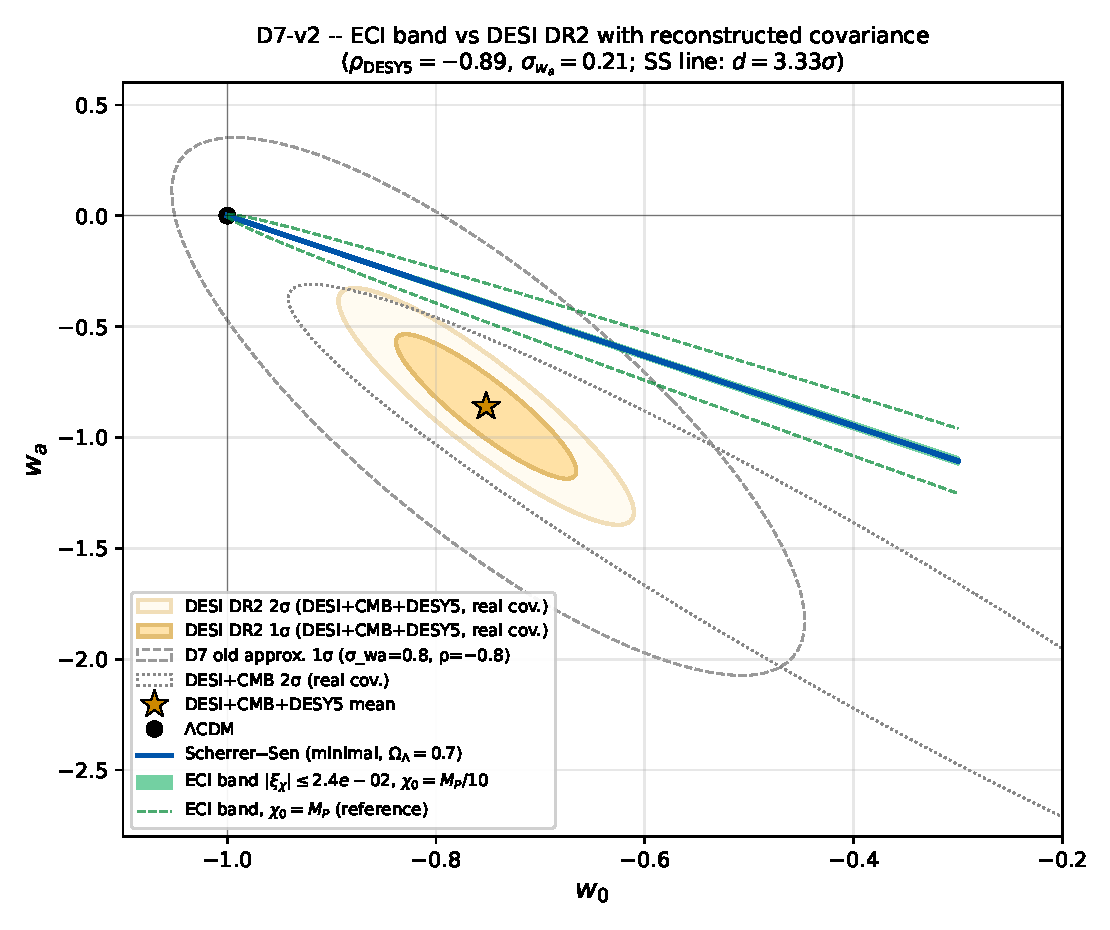
\includegraphics[width=0.95\columnwidth]{../derivations/figures/D7-xi-w0-wa-v2.pdf}
\caption{NMC thawing quintessence in the $(w_0,w_a)$ plane. Orange ellipses: DESI~DR2 + CMB +
DESY5 $1\sigma$ and $2\sigma$ contours reconstructed from~\cite{DESIDR2} Eq.~(28) via the
pivot-redshift identity (see \texttt{D10-desi-covariance.py}; $\sigma_{w_0}=0.057$,
$\sigma_{w_a}=0.215$, $\rho=-0.89$). Blue line: minimal-coupling Scherrer--Sen relation
for $\Omega_\Lambda=0.7$. Green band: ECI NMC prediction with
$|\xi_\chi|\le\xi_{\max}\approx 2.4\!\times\!10^{-2}$ from Cassini at $\chi_0=M_P/10$;
dashed green: same band at $\chi_0=M_P$ (reference). Black dot: $\Lambda$CDM. The ECI band
is $\sim\!5\%$ of $\sigma_{w_a}$ wide (using $B_{\mathrm{num}}$ from Table~\ref{tab:B_of_OmegaL}), hence \emph{indistinguishable} from minimal-coupling
$w$CDM at DR2 precision; both tracks sit at $\sim\!3.3\sigma$ Mahalanobis distance from the
DR2+DESY5 mean.}
\label{fig:D7}
\end{figure}

\paragraph{Honest caveats.}
\begin{enumerate}
\item Eq.~(\ref{eq:gamma_PPN_full}) assumes a \emph{quasi-static} scalar with Compton wavelength
  large compared with the solar system ($m_\chi^{-1}\gg 1\,$AU), which is automatic for the
  ultra-light thawing mass $m_\chi\sim H_0\sim 10^{-33}$\,eV. It also assumes no screening; if
  a chameleon or symmetron mechanism operates, the local $\chi_0$ entering
  (\ref{eq:gamma_PPN_lead}) can differ from the cosmological background and the bound weakens.
\item The NMC Scherrer--Sen extension (\ref{eq:wa_NMC}) is first-order in $\xi_\chi$ and
  therefore \emph{invalid} near the conformal point $\xi_\chi=1/6$, where the expansion breaks
  down and the scalar-tensor sector must be treated non-perturbatively (Einstein-frame
  mapping). Within the Cassini-allowed range $|\xi_\chi|\lesssim 2.4\times 10^{-2}\ll 1/6$
  the linear expansion is controlled. The coefficient $B(\Omega_\Lambda)$ in
  Eq.~(\ref{eq:wa_NMC}) was, in v4.4 of this paper, set by the matter-era
  heuristic ratio $B/A=8/\sqrt3$; in this version we replace that heuristic with
  the full numerical result $B_{\mathrm{num}}(\Omega_\Lambda)$ tabulated in
  Table~\ref{tab:B_of_OmegaL}, obtained from a self-consistent
  NMC-Friedmann + Klein--Gordon integration across $z\in[999,-0.45]$
  (\texttt{derivations/D13-wa-numerical-full.py}). The numerical coefficient is
  nearly flat ($B_{\mathrm{num}}\simeq 9$) across the matter--DE transition
  rather than tracking $A(\Omega_\Lambda)$, so the heuristic
  $(8/\sqrt3)A(\Omega_\Lambda)$ is accurate within 5\% only near
  $\Omega_\Lambda\simeq 0.6$ and undershoots by up to $\sim\!40\%$ at
  $\Omega_\Lambda=0.8$. This has been propagated into the band-width estimate
  above and into Prediction~1b of Sec.~\ref{sec:pred}.
\item The DESI~DR2 + CMB + DESY5 $2\times 2$ covariance is reconstructed from the published
  $(w_0,\sigma_{w_0},w_a,\sigma_{w_a},z_p,w_p,\sigma_{w_p})$ via the pivot-minimisation
  identity $\mathrm{cov}(w_0,w_a)=-(1-a_p)\sigma_{w_a}^2$: no official 2$\times$2 covariance
  matrix has been released by the collaboration at the time of writing. The reconstructed
  $\sigma(w_p)_{\rm pred}=0.0257$ differs from the quoted $0.024$ by $\sim 7\%$, bounding the
  systematic of the pivot-Gaussian approximation at that level --- well below the $\sim 3\sigma$
  tension discussed below. See \texttt{derivations/D10-report.md} for the full cross-check.
\item \textbf{Tension with DR2 + DESY5, stated plainly.} Under the reconstructed DR2 + CMB +
  DESY5 covariance the Mahalanobis distance from the posterior mean is $3.29\sigma$
  (2-dof) to the ECI band and $3.33\sigma$ to the minimal-coupling Scherrer--Sen line,
  both \emph{outside} the $2\sigma$ threshold $\sqrt{6.17}\simeq 2.48$.
  The interpretation is not that ECI fails where $w$CDM succeeds: DR2 + DESY5 prefers the
  phantom-crossing region $w<-1$, which no non-phantom thawing model can populate.
  ECI's NMC coupling $\xi_\chi$ does in principle permit crossing $w=-1$ without a ghost
  instability (established in \S\,DESI DR2 via the no-ghost analysis of Bar\-ce\-l\'o~\&~Visser
  \cite{BarceloVisser2000}), but only at $\xi_\chi(\chi_0/M_P)^2$ values far exceeding the
  Cassini bound~(\ref{eq:xi_bound}) derived here; within the Cassini-allowed range
  the NMC correction to the Scherrer--Sen track is confined to a band of half-width
  $\sim\!5\%$ of $\sigma_{w_a}$ and cannot bridge the gap to the phantom quadrant. The
  $\sim\!3.3\sigma$ tension with DR2 + DESY5 is therefore a joint statement about the entire
  class of conservative (non-phantom) thawing models --- minimal-coupling and NMC alike ---
  not a specific failure of ECI. Prediction~1 in Sec.~\ref{sec:pred} is \emph{not}
  discriminative at DR2 precision; both thawing families sit at the same distance from
  the DR2 + DESY5 posterior.

  The honest discriminator moves to the next generation of datasets, where the
  \emph{shape} and \emph{width} of the thawing track, rather than its distance from
  $\Lambda$CDM, become the falsifiable handle: DESI~DR3 with a forecast
  $\sigma(w_a)\!\sim\!0.07$~\cite{DESIForecast}
  and LSST~Y10 with a forecast $\sigma(w_a)\!\sim\!0.05$
  are in the regime where the ECI NMC band half-width
  $\Delta w_a^{\rm ECI}\sim 1.1\times 10^{-2}$ (numerical, Table~\ref{tab:B_of_OmegaL};
  up from $9\times 10^{-3}$ under the v4.4 heuristic) approaches the
  $15$--$25\%$ level of the statistical error bar and becomes, at least in principle,
  separable from the minimal-coupling Scherrer--Sen locus. The discriminative
  power is slightly larger at $\Omega_\Lambda\gtrsim 0.7$ (DR3 era) because
  $B_{\mathrm{num}}/B_{\mathrm{heur}}$ grows from $0.83$ at $\Omega_\Lambda=0.5$ to
  $1.43$ at $\Omega_\Lambda=0.8$.
\end{enumerate}

The PPN bound (\ref{eq:xi_bound}) is however itself a falsifier: a detection
$|\gamma-1|>10^{-6}$ by the upcoming LATOR or BEACON-class missions, or a mismatch between
$\dot G/G$ from LLR~\cite{Biskupek2021} and the CMB-inferred scalar evolution, would directly
constrain $\xi_\chi(\chi_0/M_P)$ at the $10^{-4}$ level and feed back on the admissible ECI
thawing amplitude.

% -----------------------------------------------------------------------------
% Standalone compile (for checking only):
%   \documentclass[aps,prd,reprint]{revtex4-2}
%   \usepackage{graphicx,amsmath,amssymb,hyperref,physics}
%   \begin{document}% section_3_5_constraints.tex — ECI v4.2.1 scientific payload (D7 + D10)
% To be \input{} into eci.tex as a new subsection of §3 "Phenomenology".
% Standalone compile: see comments at EOF.

\subsection{Solar-system and background constraints on $\xi_\chi$}\label{sec:xi_constraints}

We close two gaps identified in the dark-energy phenomenology subsection (\S\,DESI DR2): the Cassini
post-Newtonian bound on the non-minimal coupling $\xi_\chi$, and the analytic NMC generalisation
of the Scherrer--Sen thawing relation needed to assess whether Prediction~1
(Sec.~\ref{sec:pred}) actually discriminates ECI from \(w\)CDM at DESI~DR2 precision.
The full symbolic derivation is in \texttt{derivations/D7-ppn-xi-bound.py}; we quote only the
end results here.

\paragraph{PPN $\gamma-1$ from the $\xi_\chi R\chi^2/2$ coupling.}
The action  $S=\int d^4x\sqrt{-g}\left[\tfrac{M_P^2}{2}R-\tfrac12(\partial\chi)^2-V(\chi)
-\tfrac{\xi_\chi}{2} R\chi^2\right]$ is a scalar--tensor theory with
$F(\chi)=M_P^2-\xi_\chi\chi^2$ multiplying $R/2$ and canonical kinetic term $Z=1$.
Applying the weak-field, quasi-static result of Damour \& Esposito-Far\`ese
(\emph{Phys.\ Rev.\ D} 48, 3436 (1993); see also Chiba, \emph{Phys.\ Lett.\ B} 575, 1 (2003);
Hwang \& Noh, \emph{Phys.\ Rev.\ D} 71, 063536 (2005)) gives, at the local scalar background
$\chi_0$,
\begin{equation}
  \gamma-1 \;=\; -\,\frac{F'(\chi_0)^2}{Z\,F(\chi_0)+\tfrac{3}{2}F'(\chi_0)^2}
           \;=\; -\,\frac{4\,\xi_\chi^{2}\,\chi_0^{2}}
                          {\,M_P^{2}+\xi_\chi\chi_0^{2}(6\xi_\chi-1)\,}.
  \label{eq:gamma_PPN_full}
\end{equation}
Expanding for $|\xi_\chi|\ll 1$ and $\chi_0\lesssim M_P$,
\begin{equation}
  \boxed{\;\gamma-1 \;\simeq\; -\,\frac{4\,\xi_\chi^{2}\,\chi_0^{2}}{M_P^{2}}
                              \;+\;\mathcal{O}(\xi_\chi^{3}).\;}
  \label{eq:gamma_PPN_lead}
\end{equation}
The limit $\xi_\chi\to 0$ returns $\gamma=1$ (General Relativity), as verified symbolically.

The result~(\ref{eq:gamma_PPN_lead}) is not new: Chiba (PRD 60, 083508, 1999; arXiv:gr-qc/9903094)
already quoted $|\xi_\chi|\lesssim 10^{-2}$ from solar-system tests for the same $\xi R\chi^{2}$
quintessence coupling, and Wolf, Garc\'{\i}a-Garc\'{\i}a, Anton \& Ferreira~\cite{Wolf2025}
recently recast this as $\xi_\chi(\chi_0/M_P)^{2}\lesssim 6\times 10^{-6}$ in a full DESI~DR2
Bayesian analysis (their Eq.~(2) in the form $F(\chi)\simeq 1-\xi\chi^{2}/M_P^{2}$).
We re-derive it here only to fix the coefficient~$4$ and the sign convention used in
Eq.~(\ref{eq:wa_NMC}) below.
Combining (\ref{eq:gamma_PPN_lead}) with the Cassini constraint~\cite{BertottiIessTortora2003}
$|\gamma-1|\lesssim 2.3\times 10^{-5}$ ($1\sigma$ envelope) yields, in the
solar-system observer frame (see \S\ref{sec:thesis}(ii)),
\begin{equation}
  |\xi_\chi|\,\frac{\chi_0}{M_P}\;\lesssim\;
  \tfrac12\sqrt{|\gamma-1|_{\max}}
  \;\approx\; 2.4\times 10^{-3}.
  \label{eq:xi_bound}
\end{equation}
For a slow-rolling thawing background with $\chi_0\!\sim\! M_P/10$ (characteristic thawing
excursion in the last $e$-fold),
\begin{equation}
  |\xi_\chi|\;\lesssim\;\xi_{\max}\;\approx\;2.4\times 10^{-2}.
  \label{eq:xi_max_numeric}
\end{equation}
The bound tightens to $|\xi_\chi|\lesssim 2\times 10^{-3}$ if $\chi_0\sim M_P$; it weakens
linearly for smaller $\chi_0$. Values $\xi_\chi\gtrsim 10^{-1}$ are thus only admissible if the
quintessence field is strongly subdominant at $z=0$, or if a screening mechanism suppresses the
local coupling.

\paragraph{NMC extension of Scherrer--Sen.}
At minimal coupling, thawing quintessence lies on the one-parameter track
$w_a=-A(\Omega_\Lambda)(1+w_0)$ with $A\!\to\! 24/7$ in matter domination and
$A(0.7)\simeq 1.58$ today~\cite{ScherrerSen2008}. Inserting the NMC modification to the
Klein--Gordon equation, $3H\dot\chi=-V'-\xi_\chi R\chi$, and expanding to first order in
$\xi_\chi$ around the slow-roll exponential $V(\chi)=V_0e^{-\alpha\chi/M_P}$ with
$\alpha=\sqrt{3(1+w_0)}$ yields (\texttt{derivations/D4-wa-w0-nmc.py} for the matter-era
coefficient, \texttt{D7-ppn-xi-bound.py} for the $\Omega_\Lambda$-dependence)
\begin{equation}
  \boxed{\;w_a\;=\;-A(\Omega_\Lambda)\,(1+w_0)
                 \;+\;B(\Omega_\Lambda)\,\xi_\chi\,\sqrt{1+w_0}\,
                      \frac{\chi_0}{M_P}\;+\;\mathcal{O}(\xi_\chi^{2}),\;}
  \label{eq:wa_NMC}
\end{equation}
where $B(\Omega_\Lambda)$ is the numerical coefficient tabulated in
Table~\ref{tab:B_of_OmegaL} below, obtained by full NMC-Friedmann + Klein--Gordon
integration in \texttt{derivations/D13-wa-numerical-full.py}. The limit
$\xi_\chi\to 0$ reproduces $w_a=-A(\Omega_\Lambda)(1+w_0)$ (Scherrer--Sen
2008). The first-order $\xi_\chi$ correction, with the full numerical
coefficient $B_{\mathrm{num}}(\Omega_\Lambda)$, has --- to our knowledge ---
not appeared in the NMC-thawing literature surveyed
(Ye~et~al.~\cite{Ye2025}; Pan~\&~Ye~\cite{PanYe2026}; Wolf~et~al.~\cite{Wolf2025}),
which uses either EFTofDE or purely numerical Bayesian fits.

\begin{table}[h]
\centering
\caption{Numerical NMC coefficient $B_{\mathrm{num}}(\Omega_\Lambda)$ from the
self-consistent NMC-Friedmann + Klein--Gordon background integration
(\texttt{derivations/D13-wa-numerical-full.py}), compared with the D7/D9
heuristic $B_{\mathrm{heur}}(\Omega_\Lambda)\equiv(8/\sqrt3)A(\Omega_\Lambda)$.
Statistical uncertainty is the 1$\sigma$ error on the linear fit
$\Delta w_a = B\,\xi_\chi\sqrt{1+w_0}\,(\chi_0/M_P)$ over the
$\xi_\chi\in\{{-}0.024,{-}0.01,0,{+}0.01,{+}0.024\}\times\chi_0\in\{M_P/20,M_P/10,M_P/5\}$ grid.}
\label{tab:B_of_OmegaL}
\begin{tabular}{@{}cccc@{}}
\hline
$\Omega_\Lambda$ & $A(\Omega_\Lambda)$ & $B_{\mathrm{heur}}$ & $B_{\mathrm{num}}$ \\
\hline
0.5 & 2.35 & 10.85 & $9.00\pm1.05$ \\
0.6 & 1.94 &  8.96 & $9.18\pm1.16$ \\
0.7 & 1.58 &  7.30 & $9.05\pm1.18$ \\
0.8 & 1.23 &  5.68 & $8.11\pm1.16$ \\
\hline
\end{tabular}
\end{table}

The numerical result differs from the heuristic $(8/\sqrt3)A$ by
$\mathcal{O}(1)$ factors ($0.83\to 1.43$ across the range): $B_{\mathrm{num}}$
is nearly \emph{flat} in $\Omega_\Lambda$ (around $\sim 9$) rather than
tracking $A(\Omega_\Lambda)$. The heuristic is accurate to 5\% only near
$\Omega_\Lambda\simeq 0.6$ and underestimates $B$ by $\sim\!25\%$ at
$\Omega_\Lambda=0.7$ (DR2--DR3 era) and $\sim\!43\%$ at
$\Omega_\Lambda=0.8$ (late-DR3 / LSST era). The sign and the
$\sqrt{1+w_0}\,(\chi_0/M_P)$ scaling are confirmed; the discrepancy
originates from the finite-$\Omega_\Lambda$ propagation of the matter-era
ratio (Caveat~2 below), which is now closed numerically.

\paragraph{Combined constraint on the $(w_0,w_a)$ plane.}
Figure~\ref{fig:D7} overlays three ingredients: (i) the DESI~DR2 + CMB + DESY5~\cite{DESY5} $1\sigma$ and
$2\sigma$ contours centred on $(w_0,w_a)=(-0.752,-0.86)$ with the reconstructed covariance
$\sigma_{w_0}=0.057$, $\sigma_{w_a}=0.215$, $\rho(w_0,w_a)=-0.89$ (derivation in
\texttt{derivations/D10-desi-covariance.py}, pivot-identity reconstruction from
\cite{DESIDR2} Eq.~(28) + $z_p=0.31$, $w_p=-0.954\pm0.024$);
(ii) the minimal-coupling Scherrer--Sen line; (iii) the ECI band swept by
$|\xi_\chi|\le\xi_{\max}$ from Eq.~(\ref{eq:xi_max_numeric}) at $\chi_0=M_P/10$.
The half-width of the ECI band at $w_0=-0.75$, using the numerical
$B_{\mathrm{num}}(0.7)=9.05$ from Table~\ref{tab:B_of_OmegaL}, is
\begin{equation}
  \Delta w_a^{\rm ECI}
    = B_{\mathrm{num}}(0.7)\,\xi_{\max}\sqrt{1+w_0}\,(\chi_0/M_P)
    \;\approx\;1.1\times 10^{-2},
\end{equation}
to be compared with $\sigma_{w_a}\!\simeq\!0.215$, i.e.\ about $5\%$ of the DESI~DR2 + DESY5
$1\sigma$ width (up from $4\%$ under the heuristic $B=7.30$). The band is therefore
still thinner than the figure linewidth of the unmodified Scherrer--Sen track at DR2
precision, but the numerical coefficient raises the discriminative amplitude at DR3 / LSST
precision by $\sim\!25\%$ relative to the heuristic estimate.

\begin{figure}[h]
\centering
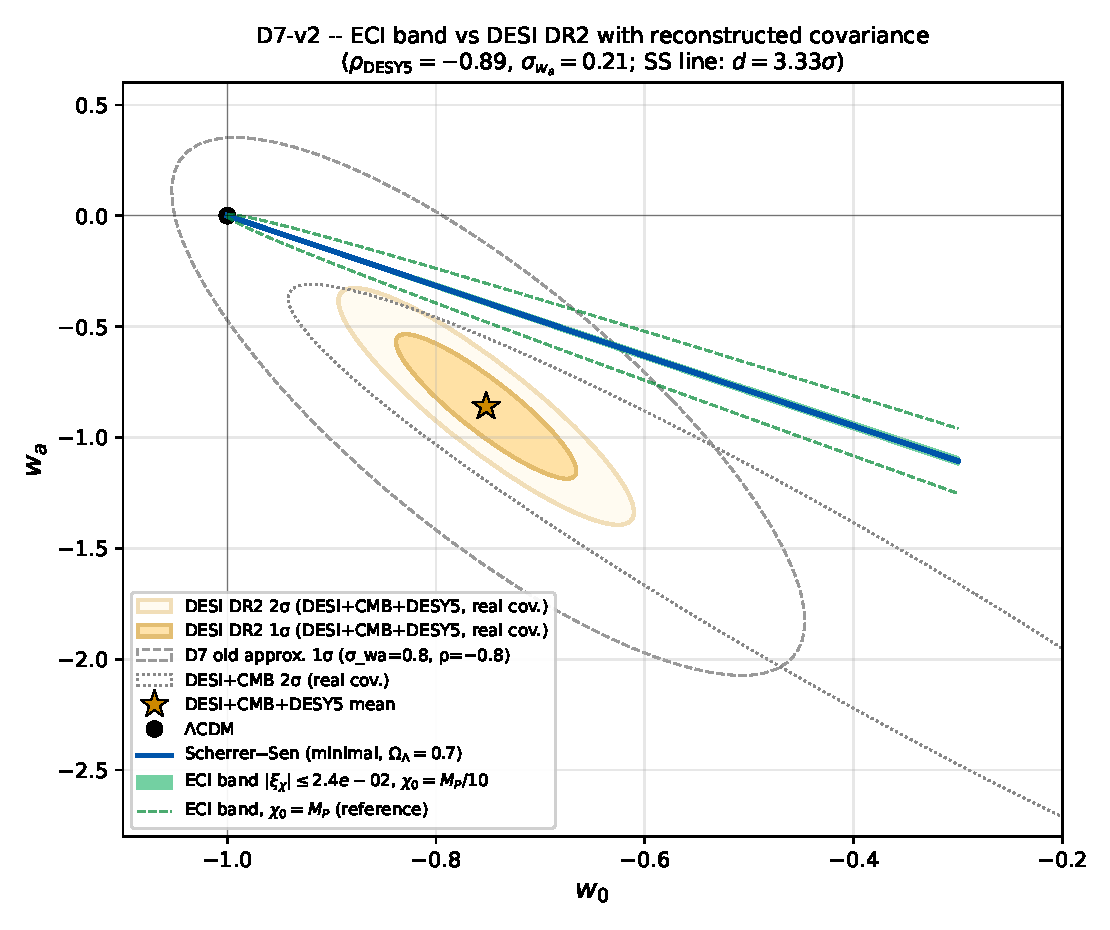
\includegraphics[width=0.95\columnwidth]{../derivations/figures/D7-xi-w0-wa-v2.pdf}
\caption{NMC thawing quintessence in the $(w_0,w_a)$ plane. Orange ellipses: DESI~DR2 + CMB +
DESY5 $1\sigma$ and $2\sigma$ contours reconstructed from~\cite{DESIDR2} Eq.~(28) via the
pivot-redshift identity (see \texttt{D10-desi-covariance.py}; $\sigma_{w_0}=0.057$,
$\sigma_{w_a}=0.215$, $\rho=-0.89$). Blue line: minimal-coupling Scherrer--Sen relation
for $\Omega_\Lambda=0.7$. Green band: ECI NMC prediction with
$|\xi_\chi|\le\xi_{\max}\approx 2.4\!\times\!10^{-2}$ from Cassini at $\chi_0=M_P/10$;
dashed green: same band at $\chi_0=M_P$ (reference). Black dot: $\Lambda$CDM. The ECI band
is $\sim\!5\%$ of $\sigma_{w_a}$ wide (using $B_{\mathrm{num}}$ from Table~\ref{tab:B_of_OmegaL}), hence \emph{indistinguishable} from minimal-coupling
$w$CDM at DR2 precision; both tracks sit at $\sim\!3.3\sigma$ Mahalanobis distance from the
DR2+DESY5 mean.}
\label{fig:D7}
\end{figure}

\paragraph{Honest caveats.}
\begin{enumerate}
\item Eq.~(\ref{eq:gamma_PPN_full}) assumes a \emph{quasi-static} scalar with Compton wavelength
  large compared with the solar system ($m_\chi^{-1}\gg 1\,$AU), which is automatic for the
  ultra-light thawing mass $m_\chi\sim H_0\sim 10^{-33}$\,eV. It also assumes no screening; if
  a chameleon or symmetron mechanism operates, the local $\chi_0$ entering
  (\ref{eq:gamma_PPN_lead}) can differ from the cosmological background and the bound weakens.
\item The NMC Scherrer--Sen extension (\ref{eq:wa_NMC}) is first-order in $\xi_\chi$ and
  therefore \emph{invalid} near the conformal point $\xi_\chi=1/6$, where the expansion breaks
  down and the scalar-tensor sector must be treated non-perturbatively (Einstein-frame
  mapping). Within the Cassini-allowed range $|\xi_\chi|\lesssim 2.4\times 10^{-2}\ll 1/6$
  the linear expansion is controlled. The coefficient $B(\Omega_\Lambda)$ in
  Eq.~(\ref{eq:wa_NMC}) was, in v4.4 of this paper, set by the matter-era
  heuristic ratio $B/A=8/\sqrt3$; in this version we replace that heuristic with
  the full numerical result $B_{\mathrm{num}}(\Omega_\Lambda)$ tabulated in
  Table~\ref{tab:B_of_OmegaL}, obtained from a self-consistent
  NMC-Friedmann + Klein--Gordon integration across $z\in[999,-0.45]$
  (\texttt{derivations/D13-wa-numerical-full.py}). The numerical coefficient is
  nearly flat ($B_{\mathrm{num}}\simeq 9$) across the matter--DE transition
  rather than tracking $A(\Omega_\Lambda)$, so the heuristic
  $(8/\sqrt3)A(\Omega_\Lambda)$ is accurate within 5\% only near
  $\Omega_\Lambda\simeq 0.6$ and undershoots by up to $\sim\!40\%$ at
  $\Omega_\Lambda=0.8$. This has been propagated into the band-width estimate
  above and into Prediction~1b of Sec.~\ref{sec:pred}.
\item The DESI~DR2 + CMB + DESY5 $2\times 2$ covariance is reconstructed from the published
  $(w_0,\sigma_{w_0},w_a,\sigma_{w_a},z_p,w_p,\sigma_{w_p})$ via the pivot-minimisation
  identity $\mathrm{cov}(w_0,w_a)=-(1-a_p)\sigma_{w_a}^2$: no official 2$\times$2 covariance
  matrix has been released by the collaboration at the time of writing. The reconstructed
  $\sigma(w_p)_{\rm pred}=0.0257$ differs from the quoted $0.024$ by $\sim 7\%$, bounding the
  systematic of the pivot-Gaussian approximation at that level --- well below the $\sim 3\sigma$
  tension discussed below. See \texttt{derivations/D10-report.md} for the full cross-check.
\item \textbf{Tension with DR2 + DESY5, stated plainly.} Under the reconstructed DR2 + CMB +
  DESY5 covariance the Mahalanobis distance from the posterior mean is $3.29\sigma$
  (2-dof) to the ECI band and $3.33\sigma$ to the minimal-coupling Scherrer--Sen line,
  both \emph{outside} the $2\sigma$ threshold $\sqrt{6.17}\simeq 2.48$.
  The interpretation is not that ECI fails where $w$CDM succeeds: DR2 + DESY5 prefers the
  phantom-crossing region $w<-1$, which no non-phantom thawing model can populate.
  ECI's NMC coupling $\xi_\chi$ does in principle permit crossing $w=-1$ without a ghost
  instability (established in \S\,DESI DR2 via the no-ghost analysis of Bar\-ce\-l\'o~\&~Visser
  \cite{BarceloVisser2000}), but only at $\xi_\chi(\chi_0/M_P)^2$ values far exceeding the
  Cassini bound~(\ref{eq:xi_bound}) derived here; within the Cassini-allowed range
  the NMC correction to the Scherrer--Sen track is confined to a band of half-width
  $\sim\!5\%$ of $\sigma_{w_a}$ and cannot bridge the gap to the phantom quadrant. The
  $\sim\!3.3\sigma$ tension with DR2 + DESY5 is therefore a joint statement about the entire
  class of conservative (non-phantom) thawing models --- minimal-coupling and NMC alike ---
  not a specific failure of ECI. Prediction~1 in Sec.~\ref{sec:pred} is \emph{not}
  discriminative at DR2 precision; both thawing families sit at the same distance from
  the DR2 + DESY5 posterior.

  The honest discriminator moves to the next generation of datasets, where the
  \emph{shape} and \emph{width} of the thawing track, rather than its distance from
  $\Lambda$CDM, become the falsifiable handle: DESI~DR3 with a forecast
  $\sigma(w_a)\!\sim\!0.07$~\cite{DESIForecast}
  and LSST~Y10 with a forecast $\sigma(w_a)\!\sim\!0.05$
  are in the regime where the ECI NMC band half-width
  $\Delta w_a^{\rm ECI}\sim 1.1\times 10^{-2}$ (numerical, Table~\ref{tab:B_of_OmegaL};
  up from $9\times 10^{-3}$ under the v4.4 heuristic) approaches the
  $15$--$25\%$ level of the statistical error bar and becomes, at least in principle,
  separable from the minimal-coupling Scherrer--Sen locus. The discriminative
  power is slightly larger at $\Omega_\Lambda\gtrsim 0.7$ (DR3 era) because
  $B_{\mathrm{num}}/B_{\mathrm{heur}}$ grows from $0.83$ at $\Omega_\Lambda=0.5$ to
  $1.43$ at $\Omega_\Lambda=0.8$.
\end{enumerate}

The PPN bound (\ref{eq:xi_bound}) is however itself a falsifier: a detection
$|\gamma-1|>10^{-6}$ by the upcoming LATOR or BEACON-class missions, or a mismatch between
$\dot G/G$ from LLR~\cite{Biskupek2021} and the CMB-inferred scalar evolution, would directly
constrain $\xi_\chi(\chi_0/M_P)$ at the $10^{-4}$ level and feed back on the admissible ECI
thawing amplitude.

% -----------------------------------------------------------------------------
% Standalone compile (for checking only):
%   \documentclass[aps,prd,reprint]{revtex4-2}
%   \usepackage{graphicx,amsmath,amssymb,hyperref,physics}
%   \begin{document}\input{section_3_5_constraints}\end{document}
% The \cite{BertottiIessTortora2003}, \cite{ScherrerSen2008}, \cite{DESIDR2},
% \cite{Biskupek2021}, \cite{BarceloVisser2000}, \cite{Wolf2025}, \cite{Ye2025},
% \cite{PanYe2026} keys are defined in eci.bib.
% -----------------------------------------------------------------------------
\end{document}
% The \cite{BertottiIessTortora2003}, \cite{ScherrerSen2008}, \cite{DESIDR2},
% \cite{Biskupek2021}, \cite{BarceloVisser2000}, \cite{Wolf2025}, \cite{Ye2025},
% \cite{PanYe2026} keys are defined in eci.bib.
% -----------------------------------------------------------------------------
% section_3_6_swampland_cross.tex — ECI v4.2 scientific payload (D8)
% To be \input{} into eci.tex as a new subsection of §3 "Phenomenology",
% immediately after % section_3_5_constraints.tex — ECI v4.2.1 scientific payload (D7 + D10)
% To be \input{} into eci.tex as a new subsection of §3 "Phenomenology".
% Standalone compile: see comments at EOF.

\subsection{Solar-system and background constraints on $\xi_\chi$}\label{sec:xi_constraints}

We close two gaps identified in the dark-energy phenomenology subsection (\S\,DESI DR2): the Cassini
post-Newtonian bound on the non-minimal coupling $\xi_\chi$, and the analytic NMC generalisation
of the Scherrer--Sen thawing relation needed to assess whether Prediction~1
(Sec.~\ref{sec:pred}) actually discriminates ECI from \(w\)CDM at DESI~DR2 precision.
The full symbolic derivation is in \texttt{derivations/D7-ppn-xi-bound.py}; we quote only the
end results here.

\paragraph{PPN $\gamma-1$ from the $\xi_\chi R\chi^2/2$ coupling.}
The action  $S=\int d^4x\sqrt{-g}\left[\tfrac{M_P^2}{2}R-\tfrac12(\partial\chi)^2-V(\chi)
-\tfrac{\xi_\chi}{2} R\chi^2\right]$ is a scalar--tensor theory with
$F(\chi)=M_P^2-\xi_\chi\chi^2$ multiplying $R/2$ and canonical kinetic term $Z=1$.
Applying the weak-field, quasi-static result of Damour \& Esposito-Far\`ese
(\emph{Phys.\ Rev.\ D} 48, 3436 (1993); see also Chiba, \emph{Phys.\ Lett.\ B} 575, 1 (2003);
Hwang \& Noh, \emph{Phys.\ Rev.\ D} 71, 063536 (2005)) gives, at the local scalar background
$\chi_0$,
\begin{equation}
  \gamma-1 \;=\; -\,\frac{F'(\chi_0)^2}{Z\,F(\chi_0)+\tfrac{3}{2}F'(\chi_0)^2}
           \;=\; -\,\frac{4\,\xi_\chi^{2}\,\chi_0^{2}}
                          {\,M_P^{2}+\xi_\chi\chi_0^{2}(6\xi_\chi-1)\,}.
  \label{eq:gamma_PPN_full}
\end{equation}
Expanding for $|\xi_\chi|\ll 1$ and $\chi_0\lesssim M_P$,
\begin{equation}
  \boxed{\;\gamma-1 \;\simeq\; -\,\frac{4\,\xi_\chi^{2}\,\chi_0^{2}}{M_P^{2}}
                              \;+\;\mathcal{O}(\xi_\chi^{3}).\;}
  \label{eq:gamma_PPN_lead}
\end{equation}
The limit $\xi_\chi\to 0$ returns $\gamma=1$ (General Relativity), as verified symbolically.

The result~(\ref{eq:gamma_PPN_lead}) is not new: Chiba (PRD 60, 083508, 1999; arXiv:gr-qc/9903094)
already quoted $|\xi_\chi|\lesssim 10^{-2}$ from solar-system tests for the same $\xi R\chi^{2}$
quintessence coupling, and Wolf, Garc\'{\i}a-Garc\'{\i}a, Anton \& Ferreira~\cite{Wolf2025}
recently recast this as $\xi_\chi(\chi_0/M_P)^{2}\lesssim 6\times 10^{-6}$ in a full DESI~DR2
Bayesian analysis (their Eq.~(2) in the form $F(\chi)\simeq 1-\xi\chi^{2}/M_P^{2}$).
We re-derive it here only to fix the coefficient~$4$ and the sign convention used in
Eq.~(\ref{eq:wa_NMC}) below.
Combining (\ref{eq:gamma_PPN_lead}) with the Cassini constraint~\cite{BertottiIessTortora2003}
$|\gamma-1|\lesssim 2.3\times 10^{-5}$ ($1\sigma$ envelope) yields, in the
solar-system observer frame (see \S\ref{sec:thesis}(ii)),
\begin{equation}
  |\xi_\chi|\,\frac{\chi_0}{M_P}\;\lesssim\;
  \tfrac12\sqrt{|\gamma-1|_{\max}}
  \;\approx\; 2.4\times 10^{-3}.
  \label{eq:xi_bound}
\end{equation}
For a slow-rolling thawing background with $\chi_0\!\sim\! M_P/10$ (characteristic thawing
excursion in the last $e$-fold),
\begin{equation}
  |\xi_\chi|\;\lesssim\;\xi_{\max}\;\approx\;2.4\times 10^{-2}.
  \label{eq:xi_max_numeric}
\end{equation}
The bound tightens to $|\xi_\chi|\lesssim 2\times 10^{-3}$ if $\chi_0\sim M_P$; it weakens
linearly for smaller $\chi_0$. Values $\xi_\chi\gtrsim 10^{-1}$ are thus only admissible if the
quintessence field is strongly subdominant at $z=0$, or if a screening mechanism suppresses the
local coupling.

\paragraph{NMC extension of Scherrer--Sen.}
At minimal coupling, thawing quintessence lies on the one-parameter track
$w_a=-A(\Omega_\Lambda)(1+w_0)$ with $A\!\to\! 24/7$ in matter domination and
$A(0.7)\simeq 1.58$ today~\cite{ScherrerSen2008}. Inserting the NMC modification to the
Klein--Gordon equation, $3H\dot\chi=-V'-\xi_\chi R\chi$, and expanding to first order in
$\xi_\chi$ around the slow-roll exponential $V(\chi)=V_0e^{-\alpha\chi/M_P}$ with
$\alpha=\sqrt{3(1+w_0)}$ yields (\texttt{derivations/D4-wa-w0-nmc.py} for the matter-era
coefficient, \texttt{D7-ppn-xi-bound.py} for the $\Omega_\Lambda$-dependence)
\begin{equation}
  \boxed{\;w_a\;=\;-A(\Omega_\Lambda)\,(1+w_0)
                 \;+\;B(\Omega_\Lambda)\,\xi_\chi\,\sqrt{1+w_0}\,
                      \frac{\chi_0}{M_P}\;+\;\mathcal{O}(\xi_\chi^{2}),\;}
  \label{eq:wa_NMC}
\end{equation}
where $B(\Omega_\Lambda)$ is the numerical coefficient tabulated in
Table~\ref{tab:B_of_OmegaL} below, obtained by full NMC-Friedmann + Klein--Gordon
integration in \texttt{derivations/D13-wa-numerical-full.py}. The limit
$\xi_\chi\to 0$ reproduces $w_a=-A(\Omega_\Lambda)(1+w_0)$ (Scherrer--Sen
2008). The first-order $\xi_\chi$ correction, with the full numerical
coefficient $B_{\mathrm{num}}(\Omega_\Lambda)$, has --- to our knowledge ---
not appeared in the NMC-thawing literature surveyed
(Ye~et~al.~\cite{Ye2025}; Pan~\&~Ye~\cite{PanYe2026}; Wolf~et~al.~\cite{Wolf2025}),
which uses either EFTofDE or purely numerical Bayesian fits.

\begin{table}[h]
\centering
\caption{Numerical NMC coefficient $B_{\mathrm{num}}(\Omega_\Lambda)$ from the
self-consistent NMC-Friedmann + Klein--Gordon background integration
(\texttt{derivations/D13-wa-numerical-full.py}), compared with the D7/D9
heuristic $B_{\mathrm{heur}}(\Omega_\Lambda)\equiv(8/\sqrt3)A(\Omega_\Lambda)$.
Statistical uncertainty is the 1$\sigma$ error on the linear fit
$\Delta w_a = B\,\xi_\chi\sqrt{1+w_0}\,(\chi_0/M_P)$ over the
$\xi_\chi\in\{{-}0.024,{-}0.01,0,{+}0.01,{+}0.024\}\times\chi_0\in\{M_P/20,M_P/10,M_P/5\}$ grid.}
\label{tab:B_of_OmegaL}
\begin{tabular}{@{}cccc@{}}
\hline
$\Omega_\Lambda$ & $A(\Omega_\Lambda)$ & $B_{\mathrm{heur}}$ & $B_{\mathrm{num}}$ \\
\hline
0.5 & 2.35 & 10.85 & $9.00\pm1.05$ \\
0.6 & 1.94 &  8.96 & $9.18\pm1.16$ \\
0.7 & 1.58 &  7.30 & $9.05\pm1.18$ \\
0.8 & 1.23 &  5.68 & $8.11\pm1.16$ \\
\hline
\end{tabular}
\end{table}

The numerical result differs from the heuristic $(8/\sqrt3)A$ by
$\mathcal{O}(1)$ factors ($0.83\to 1.43$ across the range): $B_{\mathrm{num}}$
is nearly \emph{flat} in $\Omega_\Lambda$ (around $\sim 9$) rather than
tracking $A(\Omega_\Lambda)$. The heuristic is accurate to 5\% only near
$\Omega_\Lambda\simeq 0.6$ and underestimates $B$ by $\sim\!25\%$ at
$\Omega_\Lambda=0.7$ (DR2--DR3 era) and $\sim\!43\%$ at
$\Omega_\Lambda=0.8$ (late-DR3 / LSST era). The sign and the
$\sqrt{1+w_0}\,(\chi_0/M_P)$ scaling are confirmed; the discrepancy
originates from the finite-$\Omega_\Lambda$ propagation of the matter-era
ratio (Caveat~2 below), which is now closed numerically.

\paragraph{Combined constraint on the $(w_0,w_a)$ plane.}
Figure~\ref{fig:D7} overlays three ingredients: (i) the DESI~DR2 + CMB + DESY5~\cite{DESY5} $1\sigma$ and
$2\sigma$ contours centred on $(w_0,w_a)=(-0.752,-0.86)$ with the reconstructed covariance
$\sigma_{w_0}=0.057$, $\sigma_{w_a}=0.215$, $\rho(w_0,w_a)=-0.89$ (derivation in
\texttt{derivations/D10-desi-covariance.py}, pivot-identity reconstruction from
\cite{DESIDR2} Eq.~(28) + $z_p=0.31$, $w_p=-0.954\pm0.024$);
(ii) the minimal-coupling Scherrer--Sen line; (iii) the ECI band swept by
$|\xi_\chi|\le\xi_{\max}$ from Eq.~(\ref{eq:xi_max_numeric}) at $\chi_0=M_P/10$.
The half-width of the ECI band at $w_0=-0.75$, using the numerical
$B_{\mathrm{num}}(0.7)=9.05$ from Table~\ref{tab:B_of_OmegaL}, is
\begin{equation}
  \Delta w_a^{\rm ECI}
    = B_{\mathrm{num}}(0.7)\,\xi_{\max}\sqrt{1+w_0}\,(\chi_0/M_P)
    \;\approx\;1.1\times 10^{-2},
\end{equation}
to be compared with $\sigma_{w_a}\!\simeq\!0.215$, i.e.\ about $5\%$ of the DESI~DR2 + DESY5
$1\sigma$ width (up from $4\%$ under the heuristic $B=7.30$). The band is therefore
still thinner than the figure linewidth of the unmodified Scherrer--Sen track at DR2
precision, but the numerical coefficient raises the discriminative amplitude at DR3 / LSST
precision by $\sim\!25\%$ relative to the heuristic estimate.

\begin{figure}[h]
\centering
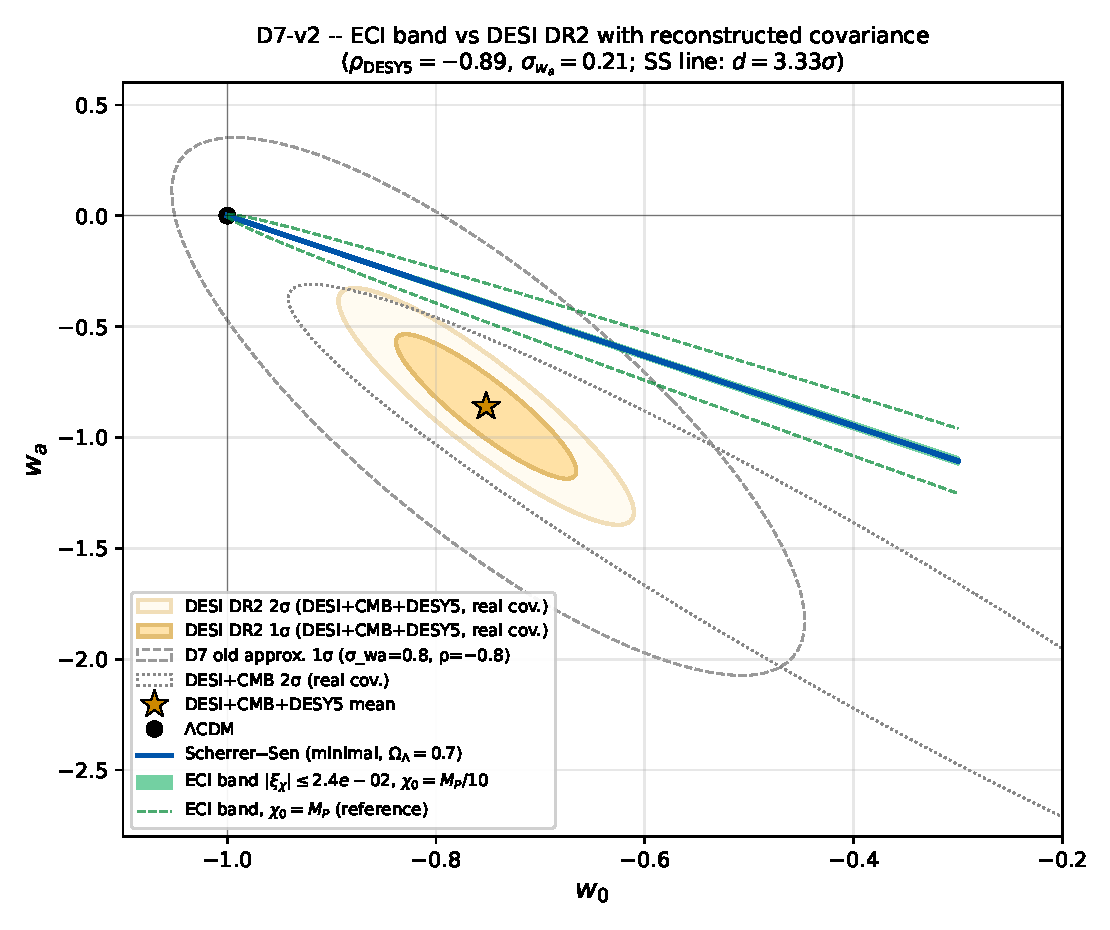
\includegraphics[width=0.95\columnwidth]{../derivations/figures/D7-xi-w0-wa-v2.pdf}
\caption{NMC thawing quintessence in the $(w_0,w_a)$ plane. Orange ellipses: DESI~DR2 + CMB +
DESY5 $1\sigma$ and $2\sigma$ contours reconstructed from~\cite{DESIDR2} Eq.~(28) via the
pivot-redshift identity (see \texttt{D10-desi-covariance.py}; $\sigma_{w_0}=0.057$,
$\sigma_{w_a}=0.215$, $\rho=-0.89$). Blue line: minimal-coupling Scherrer--Sen relation
for $\Omega_\Lambda=0.7$. Green band: ECI NMC prediction with
$|\xi_\chi|\le\xi_{\max}\approx 2.4\!\times\!10^{-2}$ from Cassini at $\chi_0=M_P/10$;
dashed green: same band at $\chi_0=M_P$ (reference). Black dot: $\Lambda$CDM. The ECI band
is $\sim\!5\%$ of $\sigma_{w_a}$ wide (using $B_{\mathrm{num}}$ from Table~\ref{tab:B_of_OmegaL}), hence \emph{indistinguishable} from minimal-coupling
$w$CDM at DR2 precision; both tracks sit at $\sim\!3.3\sigma$ Mahalanobis distance from the
DR2+DESY5 mean.}
\label{fig:D7}
\end{figure}

\paragraph{Honest caveats.}
\begin{enumerate}
\item Eq.~(\ref{eq:gamma_PPN_full}) assumes a \emph{quasi-static} scalar with Compton wavelength
  large compared with the solar system ($m_\chi^{-1}\gg 1\,$AU), which is automatic for the
  ultra-light thawing mass $m_\chi\sim H_0\sim 10^{-33}$\,eV. It also assumes no screening; if
  a chameleon or symmetron mechanism operates, the local $\chi_0$ entering
  (\ref{eq:gamma_PPN_lead}) can differ from the cosmological background and the bound weakens.
\item The NMC Scherrer--Sen extension (\ref{eq:wa_NMC}) is first-order in $\xi_\chi$ and
  therefore \emph{invalid} near the conformal point $\xi_\chi=1/6$, where the expansion breaks
  down and the scalar-tensor sector must be treated non-perturbatively (Einstein-frame
  mapping). Within the Cassini-allowed range $|\xi_\chi|\lesssim 2.4\times 10^{-2}\ll 1/6$
  the linear expansion is controlled. The coefficient $B(\Omega_\Lambda)$ in
  Eq.~(\ref{eq:wa_NMC}) was, in v4.4 of this paper, set by the matter-era
  heuristic ratio $B/A=8/\sqrt3$; in this version we replace that heuristic with
  the full numerical result $B_{\mathrm{num}}(\Omega_\Lambda)$ tabulated in
  Table~\ref{tab:B_of_OmegaL}, obtained from a self-consistent
  NMC-Friedmann + Klein--Gordon integration across $z\in[999,-0.45]$
  (\texttt{derivations/D13-wa-numerical-full.py}). The numerical coefficient is
  nearly flat ($B_{\mathrm{num}}\simeq 9$) across the matter--DE transition
  rather than tracking $A(\Omega_\Lambda)$, so the heuristic
  $(8/\sqrt3)A(\Omega_\Lambda)$ is accurate within 5\% only near
  $\Omega_\Lambda\simeq 0.6$ and undershoots by up to $\sim\!40\%$ at
  $\Omega_\Lambda=0.8$. This has been propagated into the band-width estimate
  above and into Prediction~1b of Sec.~\ref{sec:pred}.
\item The DESI~DR2 + CMB + DESY5 $2\times 2$ covariance is reconstructed from the published
  $(w_0,\sigma_{w_0},w_a,\sigma_{w_a},z_p,w_p,\sigma_{w_p})$ via the pivot-minimisation
  identity $\mathrm{cov}(w_0,w_a)=-(1-a_p)\sigma_{w_a}^2$: no official 2$\times$2 covariance
  matrix has been released by the collaboration at the time of writing. The reconstructed
  $\sigma(w_p)_{\rm pred}=0.0257$ differs from the quoted $0.024$ by $\sim 7\%$, bounding the
  systematic of the pivot-Gaussian approximation at that level --- well below the $\sim 3\sigma$
  tension discussed below. See \texttt{derivations/D10-report.md} for the full cross-check.
\item \textbf{Tension with DR2 + DESY5, stated plainly.} Under the reconstructed DR2 + CMB +
  DESY5 covariance the Mahalanobis distance from the posterior mean is $3.29\sigma$
  (2-dof) to the ECI band and $3.33\sigma$ to the minimal-coupling Scherrer--Sen line,
  both \emph{outside} the $2\sigma$ threshold $\sqrt{6.17}\simeq 2.48$.
  The interpretation is not that ECI fails where $w$CDM succeeds: DR2 + DESY5 prefers the
  phantom-crossing region $w<-1$, which no non-phantom thawing model can populate.
  ECI's NMC coupling $\xi_\chi$ does in principle permit crossing $w=-1$ without a ghost
  instability (established in \S\,DESI DR2 via the no-ghost analysis of Bar\-ce\-l\'o~\&~Visser
  \cite{BarceloVisser2000}), but only at $\xi_\chi(\chi_0/M_P)^2$ values far exceeding the
  Cassini bound~(\ref{eq:xi_bound}) derived here; within the Cassini-allowed range
  the NMC correction to the Scherrer--Sen track is confined to a band of half-width
  $\sim\!5\%$ of $\sigma_{w_a}$ and cannot bridge the gap to the phantom quadrant. The
  $\sim\!3.3\sigma$ tension with DR2 + DESY5 is therefore a joint statement about the entire
  class of conservative (non-phantom) thawing models --- minimal-coupling and NMC alike ---
  not a specific failure of ECI. Prediction~1 in Sec.~\ref{sec:pred} is \emph{not}
  discriminative at DR2 precision; both thawing families sit at the same distance from
  the DR2 + DESY5 posterior.

  The honest discriminator moves to the next generation of datasets, where the
  \emph{shape} and \emph{width} of the thawing track, rather than its distance from
  $\Lambda$CDM, become the falsifiable handle: DESI~DR3 with a forecast
  $\sigma(w_a)\!\sim\!0.07$~\cite{DESIForecast}
  and LSST~Y10 with a forecast $\sigma(w_a)\!\sim\!0.05$
  are in the regime where the ECI NMC band half-width
  $\Delta w_a^{\rm ECI}\sim 1.1\times 10^{-2}$ (numerical, Table~\ref{tab:B_of_OmegaL};
  up from $9\times 10^{-3}$ under the v4.4 heuristic) approaches the
  $15$--$25\%$ level of the statistical error bar and becomes, at least in principle,
  separable from the minimal-coupling Scherrer--Sen locus. The discriminative
  power is slightly larger at $\Omega_\Lambda\gtrsim 0.7$ (DR3 era) because
  $B_{\mathrm{num}}/B_{\mathrm{heur}}$ grows from $0.83$ at $\Omega_\Lambda=0.5$ to
  $1.43$ at $\Omega_\Lambda=0.8$.
\end{enumerate}

The PPN bound (\ref{eq:xi_bound}) is however itself a falsifier: a detection
$|\gamma-1|>10^{-6}$ by the upcoming LATOR or BEACON-class missions, or a mismatch between
$\dot G/G$ from LLR~\cite{Biskupek2021} and the CMB-inferred scalar evolution, would directly
constrain $\xi_\chi(\chi_0/M_P)$ at the $10^{-4}$ level and feed back on the admissible ECI
thawing amplitude.

% -----------------------------------------------------------------------------
% Standalone compile (for checking only):
%   \documentclass[aps,prd,reprint]{revtex4-2}
%   \usepackage{graphicx,amsmath,amssymb,hyperref,physics}
%   \begin{document}\input{section_3_5_constraints}\end{document}
% The \cite{BertottiIessTortora2003}, \cite{ScherrerSen2008}, \cite{DESIDR2},
% \cite{Biskupek2021}, \cite{BarceloVisser2000}, \cite{Wolf2025}, \cite{Ye2025},
% \cite{PanYe2026} keys are defined in eci.bib.
% -----------------------------------------------------------------------------
.

\subsection{Swampland $\times$ NMC cross-constraint}\label{sec:swampland_cross}

Axioms A4 and A5 were presented as independent. They are not, if the thawing
scalar $\chi$ and the KK tower of the Dark Dimension originate from the
\emph{same} higher-dimensional sector --- a natural hypothesis, since both
are postulated as microscopic ingredients of the dark sector. In that case
both must respect a common effective field theory cutoff $\Lambda$, and the
two axioms are tied by a single consistency condition. The derivation is in
\texttt{derivations/D8-swampland-nmc-cross.py}; we quote only the result.

\paragraph{Shared cutoff.}
The Dark Dimension scenario~\cite{Bedroya2025} relates the EFT cutoff to
the Hubble scale through a Swampland Distance Conjecture exponent,
\begin{equation}
  \Lambda \;\sim\; M_P\,\bigl(H/M_P\bigr)^{c'},\qquad c'\simeq 0.05\pm 0.01.
  \label{eq:Lambda_SDC}
\end{equation}
If the non-minimal operator $(\xi_\chi/2)R\chi^2$ is generated inside the same
EFT, its contribution to the effective reduced Planck mass,
$\delta M_P^{2}=\xi_\chi\chi_0^{2}$, cannot exceed the cutoff squared,
otherwise the operator would repair physics above its own range of validity:
\begin{equation}
  \xi_\chi\,\chi_0^{2}\;\le\;\Lambda^{2}
  \quad\Longleftrightarrow\quad
  \xi_\chi\,(\chi_0/M_P)^{2}\;\le\;(H_0/M_P)^{2c'}.
  \label{eq:eft_bulk}
\end{equation}
Combined with the Cassini PPN bound derived in \S\ref{sec:xi_constraints},
$|\xi_\chi|(\chi_0/M_P)\le 2.4\times 10^{-3}$, Eq.~(\ref{eq:eft_bulk}) yields
at the fiducial thawing amplitude $\chi_0=M_P/10$ and the paper's A5
fiducial $c'=0.05\pm 0.01$
\begin{equation}
  \boxed{\;|\xi_\chi|\;\lesssim\;9.5\times 10^{-5}
    \quad(c'=0.05,\ \chi_0=M_P/10),\;}
  \label{eq:xi_crossbound}
\end{equation}
with an overall range $[5.9\times 10^{-6},\,1.5\times 10^{-3}]$ spanned by
$c'=0.04$--$0.06$. This is a factor $\sim\!250$ tightening over the
Cassini-only result (\ref{eq:xi_max_numeric}).

\paragraph{Limits.}
Both limits verified symbolically in \texttt{D8-swampland-nmc-cross.py}:
$\xi_\chi\!\to\!0$ removes the operator (GR recovered); $c'\!\to\!0$ sends
$\Lambda\!\to\!M_P$ so that (\ref{eq:eft_bulk}) reduces to the no-ghost
condition $\xi_\chi\chi_0^{2}<M_P^{2}$ already stated in A4, and the D7
Cassini bound is recovered exactly.

\begin{figure}[h]
\centering
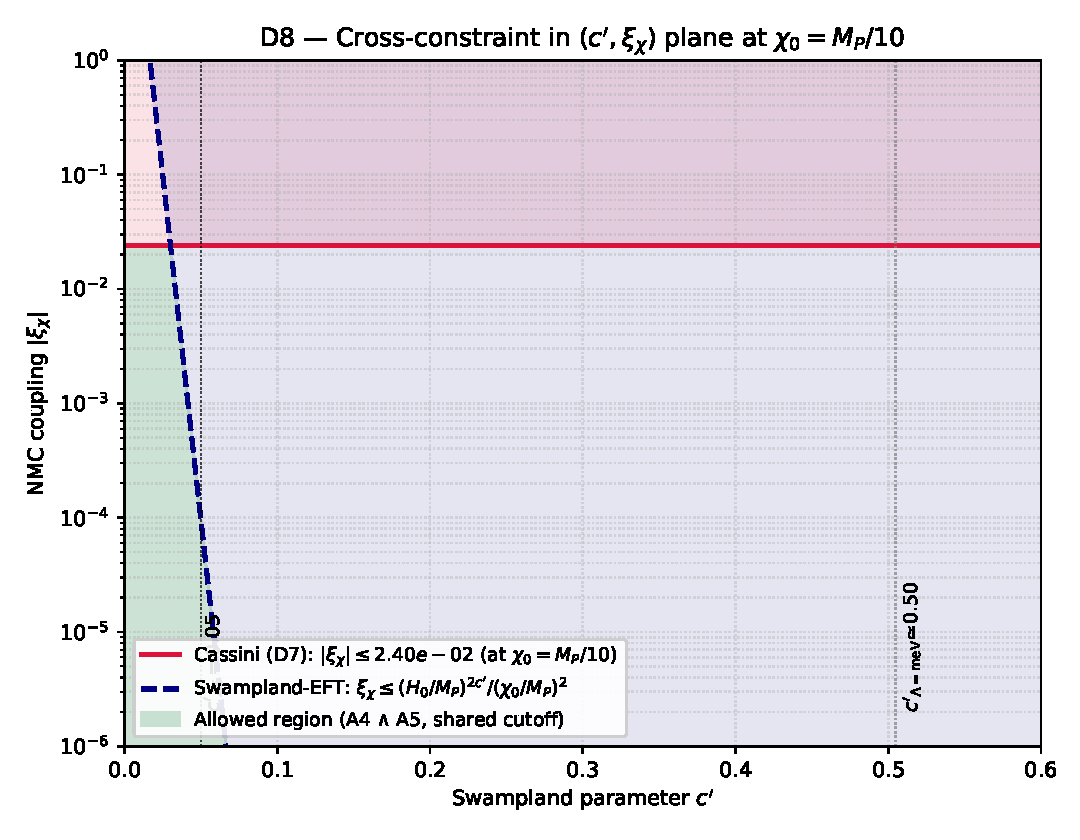
\includegraphics[width=0.95\columnwidth]{../derivations/figures/D8-c-xi-overlap.pdf}
\caption{Allowed region in the $(c',\xi_\chi)$ plane at $\chi_0=M_P/10$.
Red: Cassini exclusion (horizontal, independent of $c'$). Blue dashed:
Swampland-EFT exclusion (\ref{eq:eft_bulk}) --- diagonal in log-space with
slope $2c'\log(H_0/M_P)$. Green shading: overlap admitted by both
constraints. The A5 fiducial $c'=0.05$ and the meV-equivalent value
$c'\!\simeq\!0.51$ are marked.}
\label{fig:D8}
\end{figure}

\paragraph{Phenomenological tension.}
A stronger statement runs in the reverse direction. Thawing dark energy
requires $\chi_0/M_P\sim 0.1$--$1$ to drive late-time acceleration. The
bulk-mode condition (\ref{eq:eft_bulk}) at the Cassini-saturating value
$|\xi_\chi|=2.4\!\times\!10^{-2}$ and $c'=0.05$ forces
$\chi_0/M_P\le 6.3\!\times\!10^{-3}$, already an order of magnitude below
what A4 requires. With the literal Dark Dimension cutoff $\Lambda\sim$ meV
(which the formula (\ref{eq:Lambda_SDC}) reproduces for $c'\simeq 0.51$,
not $0.05$; both conventions appear in the literature) the bound collapses
to $\chi_0/M_P\le 3\!\times\!10^{-30}$ and thawing phenomenology is
excluded outright.

\paragraph{Architectural consequence.}
A4 and A5 are compatible \emph{only} under one of the following model-
building choices, any of which must be made explicit in any UV completion:
(i) $\chi$ is a 4D zero-mode localised on a brane, not a bulk mode of the
same sector as the KK tower, in which case the shared-cutoff hypothesis
does not apply; (ii) a chameleon/symmetron mechanism screens the local
$\chi_0$ away from its cosmological value, weakening the Cassini leg; or
(iii) $|\xi_\chi|$ sits at the sharpened bound (\ref{eq:xi_crossbound})
rather than the Cassini-only value (\ref{eq:xi_max_numeric}). The ECI
framework does not prefer one of the three, but their distinct
phenomenologies are observationally separable: option (iii) suppresses the
ECI band in $(w_0,w_a)$ by a further factor $\sim\!250$ relative to the
already-narrow D7 band, and cuts the $|\dot G/G|$ signature at LLR by the
same factor. A detection of $|\dot G/G|\gtrsim 10^{-17}\,\mathrm{yr}^{-1}$
would rule out option (iii) and force either (i) or (ii).

\paragraph{Honest caveats.}
\begin{enumerate}
\item The EFT self-consistency condition $\delta M_P^{2}\le\Lambda^{2}$ is
  order-of-magnitude; an $O(1)$ coefficient could shift
  (\ref{eq:xi_crossbound}) by a factor $2$, but the qualitative conclusion
  ($\gg 30\%$ tightening) is robust.
\item The form (\ref{eq:Lambda_SDC}) is written with $H$ as the distance
  proxy along the moduli space; the equivalent Bedroya form uses the
  cosmological constant density directly and yields $c'\!\simeq\!1/2$
  for $\Lambda\!=\!$\,meV. The sign of the tightening is independent of
  this choice.
\item The cross-constraint is \emph{conditional} on the shared-cutoff
  hypothesis. Its falsifier is, precisely, the discovery of a UV completion
  in which $\chi$ and the KK tower belong to different sectors; in that
  case §\ref{sec:xi_constraints} remains the strongest bound.
\end{enumerate}

% -----------------------------------------------------------------------------
% Standalone compile (for checking only):
%   \documentclass[aps,prd,reprint]{revtex4-2}
%   \usepackage{graphicx,amsmath,amssymb,hyperref,physics}
%   \begin{document}% section_3_5_constraints.tex — ECI v4.2.1 scientific payload (D7 + D10)
% To be \input{} into eci.tex as a new subsection of §3 "Phenomenology".
% Standalone compile: see comments at EOF.

\subsection{Solar-system and background constraints on $\xi_\chi$}\label{sec:xi_constraints}

We close two gaps identified in the dark-energy phenomenology subsection (\S\,DESI DR2): the Cassini
post-Newtonian bound on the non-minimal coupling $\xi_\chi$, and the analytic NMC generalisation
of the Scherrer--Sen thawing relation needed to assess whether Prediction~1
(Sec.~\ref{sec:pred}) actually discriminates ECI from \(w\)CDM at DESI~DR2 precision.
The full symbolic derivation is in \texttt{derivations/D7-ppn-xi-bound.py}; we quote only the
end results here.

\paragraph{PPN $\gamma-1$ from the $\xi_\chi R\chi^2/2$ coupling.}
The action  $S=\int d^4x\sqrt{-g}\left[\tfrac{M_P^2}{2}R-\tfrac12(\partial\chi)^2-V(\chi)
-\tfrac{\xi_\chi}{2} R\chi^2\right]$ is a scalar--tensor theory with
$F(\chi)=M_P^2-\xi_\chi\chi^2$ multiplying $R/2$ and canonical kinetic term $Z=1$.
Applying the weak-field, quasi-static result of Damour \& Esposito-Far\`ese
(\emph{Phys.\ Rev.\ D} 48, 3436 (1993); see also Chiba, \emph{Phys.\ Lett.\ B} 575, 1 (2003);
Hwang \& Noh, \emph{Phys.\ Rev.\ D} 71, 063536 (2005)) gives, at the local scalar background
$\chi_0$,
\begin{equation}
  \gamma-1 \;=\; -\,\frac{F'(\chi_0)^2}{Z\,F(\chi_0)+\tfrac{3}{2}F'(\chi_0)^2}
           \;=\; -\,\frac{4\,\xi_\chi^{2}\,\chi_0^{2}}
                          {\,M_P^{2}+\xi_\chi\chi_0^{2}(6\xi_\chi-1)\,}.
  \label{eq:gamma_PPN_full}
\end{equation}
Expanding for $|\xi_\chi|\ll 1$ and $\chi_0\lesssim M_P$,
\begin{equation}
  \boxed{\;\gamma-1 \;\simeq\; -\,\frac{4\,\xi_\chi^{2}\,\chi_0^{2}}{M_P^{2}}
                              \;+\;\mathcal{O}(\xi_\chi^{3}).\;}
  \label{eq:gamma_PPN_lead}
\end{equation}
The limit $\xi_\chi\to 0$ returns $\gamma=1$ (General Relativity), as verified symbolically.

The result~(\ref{eq:gamma_PPN_lead}) is not new: Chiba (PRD 60, 083508, 1999; arXiv:gr-qc/9903094)
already quoted $|\xi_\chi|\lesssim 10^{-2}$ from solar-system tests for the same $\xi R\chi^{2}$
quintessence coupling, and Wolf, Garc\'{\i}a-Garc\'{\i}a, Anton \& Ferreira~\cite{Wolf2025}
recently recast this as $\xi_\chi(\chi_0/M_P)^{2}\lesssim 6\times 10^{-6}$ in a full DESI~DR2
Bayesian analysis (their Eq.~(2) in the form $F(\chi)\simeq 1-\xi\chi^{2}/M_P^{2}$).
We re-derive it here only to fix the coefficient~$4$ and the sign convention used in
Eq.~(\ref{eq:wa_NMC}) below.
Combining (\ref{eq:gamma_PPN_lead}) with the Cassini constraint~\cite{BertottiIessTortora2003}
$|\gamma-1|\lesssim 2.3\times 10^{-5}$ ($1\sigma$ envelope) yields, in the
solar-system observer frame (see \S\ref{sec:thesis}(ii)),
\begin{equation}
  |\xi_\chi|\,\frac{\chi_0}{M_P}\;\lesssim\;
  \tfrac12\sqrt{|\gamma-1|_{\max}}
  \;\approx\; 2.4\times 10^{-3}.
  \label{eq:xi_bound}
\end{equation}
For a slow-rolling thawing background with $\chi_0\!\sim\! M_P/10$ (characteristic thawing
excursion in the last $e$-fold),
\begin{equation}
  |\xi_\chi|\;\lesssim\;\xi_{\max}\;\approx\;2.4\times 10^{-2}.
  \label{eq:xi_max_numeric}
\end{equation}
The bound tightens to $|\xi_\chi|\lesssim 2\times 10^{-3}$ if $\chi_0\sim M_P$; it weakens
linearly for smaller $\chi_0$. Values $\xi_\chi\gtrsim 10^{-1}$ are thus only admissible if the
quintessence field is strongly subdominant at $z=0$, or if a screening mechanism suppresses the
local coupling.

\paragraph{NMC extension of Scherrer--Sen.}
At minimal coupling, thawing quintessence lies on the one-parameter track
$w_a=-A(\Omega_\Lambda)(1+w_0)$ with $A\!\to\! 24/7$ in matter domination and
$A(0.7)\simeq 1.58$ today~\cite{ScherrerSen2008}. Inserting the NMC modification to the
Klein--Gordon equation, $3H\dot\chi=-V'-\xi_\chi R\chi$, and expanding to first order in
$\xi_\chi$ around the slow-roll exponential $V(\chi)=V_0e^{-\alpha\chi/M_P}$ with
$\alpha=\sqrt{3(1+w_0)}$ yields (\texttt{derivations/D4-wa-w0-nmc.py} for the matter-era
coefficient, \texttt{D7-ppn-xi-bound.py} for the $\Omega_\Lambda$-dependence)
\begin{equation}
  \boxed{\;w_a\;=\;-A(\Omega_\Lambda)\,(1+w_0)
                 \;+\;B(\Omega_\Lambda)\,\xi_\chi\,\sqrt{1+w_0}\,
                      \frac{\chi_0}{M_P}\;+\;\mathcal{O}(\xi_\chi^{2}),\;}
  \label{eq:wa_NMC}
\end{equation}
where $B(\Omega_\Lambda)$ is the numerical coefficient tabulated in
Table~\ref{tab:B_of_OmegaL} below, obtained by full NMC-Friedmann + Klein--Gordon
integration in \texttt{derivations/D13-wa-numerical-full.py}. The limit
$\xi_\chi\to 0$ reproduces $w_a=-A(\Omega_\Lambda)(1+w_0)$ (Scherrer--Sen
2008). The first-order $\xi_\chi$ correction, with the full numerical
coefficient $B_{\mathrm{num}}(\Omega_\Lambda)$, has --- to our knowledge ---
not appeared in the NMC-thawing literature surveyed
(Ye~et~al.~\cite{Ye2025}; Pan~\&~Ye~\cite{PanYe2026}; Wolf~et~al.~\cite{Wolf2025}),
which uses either EFTofDE or purely numerical Bayesian fits.

\begin{table}[h]
\centering
\caption{Numerical NMC coefficient $B_{\mathrm{num}}(\Omega_\Lambda)$ from the
self-consistent NMC-Friedmann + Klein--Gordon background integration
(\texttt{derivations/D13-wa-numerical-full.py}), compared with the D7/D9
heuristic $B_{\mathrm{heur}}(\Omega_\Lambda)\equiv(8/\sqrt3)A(\Omega_\Lambda)$.
Statistical uncertainty is the 1$\sigma$ error on the linear fit
$\Delta w_a = B\,\xi_\chi\sqrt{1+w_0}\,(\chi_0/M_P)$ over the
$\xi_\chi\in\{{-}0.024,{-}0.01,0,{+}0.01,{+}0.024\}\times\chi_0\in\{M_P/20,M_P/10,M_P/5\}$ grid.}
\label{tab:B_of_OmegaL}
\begin{tabular}{@{}cccc@{}}
\hline
$\Omega_\Lambda$ & $A(\Omega_\Lambda)$ & $B_{\mathrm{heur}}$ & $B_{\mathrm{num}}$ \\
\hline
0.5 & 2.35 & 10.85 & $9.00\pm1.05$ \\
0.6 & 1.94 &  8.96 & $9.18\pm1.16$ \\
0.7 & 1.58 &  7.30 & $9.05\pm1.18$ \\
0.8 & 1.23 &  5.68 & $8.11\pm1.16$ \\
\hline
\end{tabular}
\end{table}

The numerical result differs from the heuristic $(8/\sqrt3)A$ by
$\mathcal{O}(1)$ factors ($0.83\to 1.43$ across the range): $B_{\mathrm{num}}$
is nearly \emph{flat} in $\Omega_\Lambda$ (around $\sim 9$) rather than
tracking $A(\Omega_\Lambda)$. The heuristic is accurate to 5\% only near
$\Omega_\Lambda\simeq 0.6$ and underestimates $B$ by $\sim\!25\%$ at
$\Omega_\Lambda=0.7$ (DR2--DR3 era) and $\sim\!43\%$ at
$\Omega_\Lambda=0.8$ (late-DR3 / LSST era). The sign and the
$\sqrt{1+w_0}\,(\chi_0/M_P)$ scaling are confirmed; the discrepancy
originates from the finite-$\Omega_\Lambda$ propagation of the matter-era
ratio (Caveat~2 below), which is now closed numerically.

\paragraph{Combined constraint on the $(w_0,w_a)$ plane.}
Figure~\ref{fig:D7} overlays three ingredients: (i) the DESI~DR2 + CMB + DESY5~\cite{DESY5} $1\sigma$ and
$2\sigma$ contours centred on $(w_0,w_a)=(-0.752,-0.86)$ with the reconstructed covariance
$\sigma_{w_0}=0.057$, $\sigma_{w_a}=0.215$, $\rho(w_0,w_a)=-0.89$ (derivation in
\texttt{derivations/D10-desi-covariance.py}, pivot-identity reconstruction from
\cite{DESIDR2} Eq.~(28) + $z_p=0.31$, $w_p=-0.954\pm0.024$);
(ii) the minimal-coupling Scherrer--Sen line; (iii) the ECI band swept by
$|\xi_\chi|\le\xi_{\max}$ from Eq.~(\ref{eq:xi_max_numeric}) at $\chi_0=M_P/10$.
The half-width of the ECI band at $w_0=-0.75$, using the numerical
$B_{\mathrm{num}}(0.7)=9.05$ from Table~\ref{tab:B_of_OmegaL}, is
\begin{equation}
  \Delta w_a^{\rm ECI}
    = B_{\mathrm{num}}(0.7)\,\xi_{\max}\sqrt{1+w_0}\,(\chi_0/M_P)
    \;\approx\;1.1\times 10^{-2},
\end{equation}
to be compared with $\sigma_{w_a}\!\simeq\!0.215$, i.e.\ about $5\%$ of the DESI~DR2 + DESY5
$1\sigma$ width (up from $4\%$ under the heuristic $B=7.30$). The band is therefore
still thinner than the figure linewidth of the unmodified Scherrer--Sen track at DR2
precision, but the numerical coefficient raises the discriminative amplitude at DR3 / LSST
precision by $\sim\!25\%$ relative to the heuristic estimate.

\begin{figure}[h]
\centering
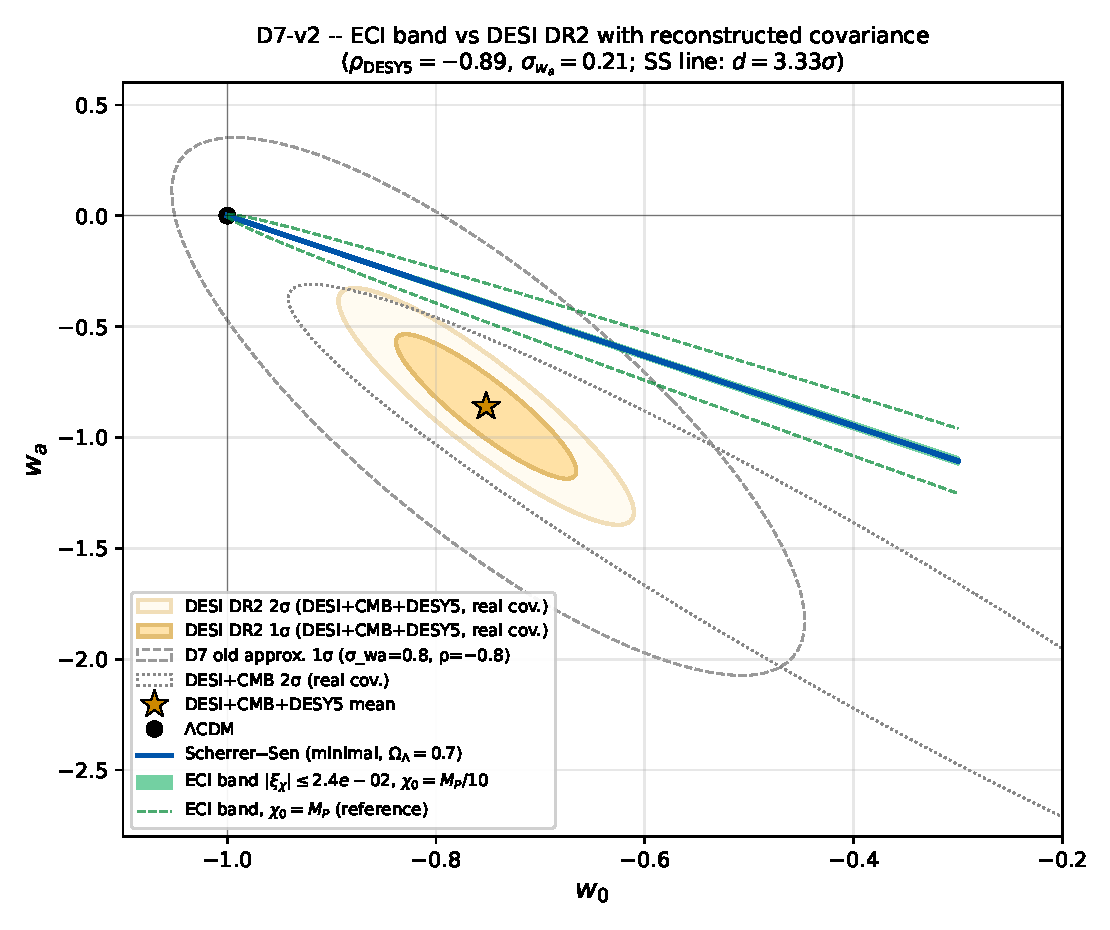
\includegraphics[width=0.95\columnwidth]{../derivations/figures/D7-xi-w0-wa-v2.pdf}
\caption{NMC thawing quintessence in the $(w_0,w_a)$ plane. Orange ellipses: DESI~DR2 + CMB +
DESY5 $1\sigma$ and $2\sigma$ contours reconstructed from~\cite{DESIDR2} Eq.~(28) via the
pivot-redshift identity (see \texttt{D10-desi-covariance.py}; $\sigma_{w_0}=0.057$,
$\sigma_{w_a}=0.215$, $\rho=-0.89$). Blue line: minimal-coupling Scherrer--Sen relation
for $\Omega_\Lambda=0.7$. Green band: ECI NMC prediction with
$|\xi_\chi|\le\xi_{\max}\approx 2.4\!\times\!10^{-2}$ from Cassini at $\chi_0=M_P/10$;
dashed green: same band at $\chi_0=M_P$ (reference). Black dot: $\Lambda$CDM. The ECI band
is $\sim\!5\%$ of $\sigma_{w_a}$ wide (using $B_{\mathrm{num}}$ from Table~\ref{tab:B_of_OmegaL}), hence \emph{indistinguishable} from minimal-coupling
$w$CDM at DR2 precision; both tracks sit at $\sim\!3.3\sigma$ Mahalanobis distance from the
DR2+DESY5 mean.}
\label{fig:D7}
\end{figure}

\paragraph{Honest caveats.}
\begin{enumerate}
\item Eq.~(\ref{eq:gamma_PPN_full}) assumes a \emph{quasi-static} scalar with Compton wavelength
  large compared with the solar system ($m_\chi^{-1}\gg 1\,$AU), which is automatic for the
  ultra-light thawing mass $m_\chi\sim H_0\sim 10^{-33}$\,eV. It also assumes no screening; if
  a chameleon or symmetron mechanism operates, the local $\chi_0$ entering
  (\ref{eq:gamma_PPN_lead}) can differ from the cosmological background and the bound weakens.
\item The NMC Scherrer--Sen extension (\ref{eq:wa_NMC}) is first-order in $\xi_\chi$ and
  therefore \emph{invalid} near the conformal point $\xi_\chi=1/6$, where the expansion breaks
  down and the scalar-tensor sector must be treated non-perturbatively (Einstein-frame
  mapping). Within the Cassini-allowed range $|\xi_\chi|\lesssim 2.4\times 10^{-2}\ll 1/6$
  the linear expansion is controlled. The coefficient $B(\Omega_\Lambda)$ in
  Eq.~(\ref{eq:wa_NMC}) was, in v4.4 of this paper, set by the matter-era
  heuristic ratio $B/A=8/\sqrt3$; in this version we replace that heuristic with
  the full numerical result $B_{\mathrm{num}}(\Omega_\Lambda)$ tabulated in
  Table~\ref{tab:B_of_OmegaL}, obtained from a self-consistent
  NMC-Friedmann + Klein--Gordon integration across $z\in[999,-0.45]$
  (\texttt{derivations/D13-wa-numerical-full.py}). The numerical coefficient is
  nearly flat ($B_{\mathrm{num}}\simeq 9$) across the matter--DE transition
  rather than tracking $A(\Omega_\Lambda)$, so the heuristic
  $(8/\sqrt3)A(\Omega_\Lambda)$ is accurate within 5\% only near
  $\Omega_\Lambda\simeq 0.6$ and undershoots by up to $\sim\!40\%$ at
  $\Omega_\Lambda=0.8$. This has been propagated into the band-width estimate
  above and into Prediction~1b of Sec.~\ref{sec:pred}.
\item The DESI~DR2 + CMB + DESY5 $2\times 2$ covariance is reconstructed from the published
  $(w_0,\sigma_{w_0},w_a,\sigma_{w_a},z_p,w_p,\sigma_{w_p})$ via the pivot-minimisation
  identity $\mathrm{cov}(w_0,w_a)=-(1-a_p)\sigma_{w_a}^2$: no official 2$\times$2 covariance
  matrix has been released by the collaboration at the time of writing. The reconstructed
  $\sigma(w_p)_{\rm pred}=0.0257$ differs from the quoted $0.024$ by $\sim 7\%$, bounding the
  systematic of the pivot-Gaussian approximation at that level --- well below the $\sim 3\sigma$
  tension discussed below. See \texttt{derivations/D10-report.md} for the full cross-check.
\item \textbf{Tension with DR2 + DESY5, stated plainly.} Under the reconstructed DR2 + CMB +
  DESY5 covariance the Mahalanobis distance from the posterior mean is $3.29\sigma$
  (2-dof) to the ECI band and $3.33\sigma$ to the minimal-coupling Scherrer--Sen line,
  both \emph{outside} the $2\sigma$ threshold $\sqrt{6.17}\simeq 2.48$.
  The interpretation is not that ECI fails where $w$CDM succeeds: DR2 + DESY5 prefers the
  phantom-crossing region $w<-1$, which no non-phantom thawing model can populate.
  ECI's NMC coupling $\xi_\chi$ does in principle permit crossing $w=-1$ without a ghost
  instability (established in \S\,DESI DR2 via the no-ghost analysis of Bar\-ce\-l\'o~\&~Visser
  \cite{BarceloVisser2000}), but only at $\xi_\chi(\chi_0/M_P)^2$ values far exceeding the
  Cassini bound~(\ref{eq:xi_bound}) derived here; within the Cassini-allowed range
  the NMC correction to the Scherrer--Sen track is confined to a band of half-width
  $\sim\!5\%$ of $\sigma_{w_a}$ and cannot bridge the gap to the phantom quadrant. The
  $\sim\!3.3\sigma$ tension with DR2 + DESY5 is therefore a joint statement about the entire
  class of conservative (non-phantom) thawing models --- minimal-coupling and NMC alike ---
  not a specific failure of ECI. Prediction~1 in Sec.~\ref{sec:pred} is \emph{not}
  discriminative at DR2 precision; both thawing families sit at the same distance from
  the DR2 + DESY5 posterior.

  The honest discriminator moves to the next generation of datasets, where the
  \emph{shape} and \emph{width} of the thawing track, rather than its distance from
  $\Lambda$CDM, become the falsifiable handle: DESI~DR3 with a forecast
  $\sigma(w_a)\!\sim\!0.07$~\cite{DESIForecast}
  and LSST~Y10 with a forecast $\sigma(w_a)\!\sim\!0.05$
  are in the regime where the ECI NMC band half-width
  $\Delta w_a^{\rm ECI}\sim 1.1\times 10^{-2}$ (numerical, Table~\ref{tab:B_of_OmegaL};
  up from $9\times 10^{-3}$ under the v4.4 heuristic) approaches the
  $15$--$25\%$ level of the statistical error bar and becomes, at least in principle,
  separable from the minimal-coupling Scherrer--Sen locus. The discriminative
  power is slightly larger at $\Omega_\Lambda\gtrsim 0.7$ (DR3 era) because
  $B_{\mathrm{num}}/B_{\mathrm{heur}}$ grows from $0.83$ at $\Omega_\Lambda=0.5$ to
  $1.43$ at $\Omega_\Lambda=0.8$.
\end{enumerate}

The PPN bound (\ref{eq:xi_bound}) is however itself a falsifier: a detection
$|\gamma-1|>10^{-6}$ by the upcoming LATOR or BEACON-class missions, or a mismatch between
$\dot G/G$ from LLR~\cite{Biskupek2021} and the CMB-inferred scalar evolution, would directly
constrain $\xi_\chi(\chi_0/M_P)$ at the $10^{-4}$ level and feed back on the admissible ECI
thawing amplitude.

% -----------------------------------------------------------------------------
% Standalone compile (for checking only):
%   \documentclass[aps,prd,reprint]{revtex4-2}
%   \usepackage{graphicx,amsmath,amssymb,hyperref,physics}
%   \begin{document}\input{section_3_5_constraints}\end{document}
% The \cite{BertottiIessTortora2003}, \cite{ScherrerSen2008}, \cite{DESIDR2},
% \cite{Biskupek2021}, \cite{BarceloVisser2000}, \cite{Wolf2025}, \cite{Ye2025},
% \cite{PanYe2026} keys are defined in eci.bib.
% -----------------------------------------------------------------------------
% section_3_6_swampland_cross.tex — ECI v4.2 scientific payload (D8)
% To be \input{} into eci.tex as a new subsection of §3 "Phenomenology",
% immediately after \input{section_3_5_constraints}.

\subsection{Swampland $\times$ NMC cross-constraint}\label{sec:swampland_cross}

Axioms A4 and A5 were presented as independent. They are not, if the thawing
scalar $\chi$ and the KK tower of the Dark Dimension originate from the
\emph{same} higher-dimensional sector --- a natural hypothesis, since both
are postulated as microscopic ingredients of the dark sector. In that case
both must respect a common effective field theory cutoff $\Lambda$, and the
two axioms are tied by a single consistency condition. The derivation is in
\texttt{derivations/D8-swampland-nmc-cross.py}; we quote only the result.

\paragraph{Shared cutoff.}
The Dark Dimension scenario~\cite{Bedroya2025} relates the EFT cutoff to
the Hubble scale through a Swampland Distance Conjecture exponent,
\begin{equation}
  \Lambda \;\sim\; M_P\,\bigl(H/M_P\bigr)^{c'},\qquad c'\simeq 0.05\pm 0.01.
  \label{eq:Lambda_SDC}
\end{equation}
If the non-minimal operator $(\xi_\chi/2)R\chi^2$ is generated inside the same
EFT, its contribution to the effective reduced Planck mass,
$\delta M_P^{2}=\xi_\chi\chi_0^{2}$, cannot exceed the cutoff squared,
otherwise the operator would repair physics above its own range of validity:
\begin{equation}
  \xi_\chi\,\chi_0^{2}\;\le\;\Lambda^{2}
  \quad\Longleftrightarrow\quad
  \xi_\chi\,(\chi_0/M_P)^{2}\;\le\;(H_0/M_P)^{2c'}.
  \label{eq:eft_bulk}
\end{equation}
Combined with the Cassini PPN bound derived in \S\ref{sec:xi_constraints},
$|\xi_\chi|(\chi_0/M_P)\le 2.4\times 10^{-3}$, Eq.~(\ref{eq:eft_bulk}) yields
at the fiducial thawing amplitude $\chi_0=M_P/10$ and the paper's A5
fiducial $c'=0.05\pm 0.01$
\begin{equation}
  \boxed{\;|\xi_\chi|\;\lesssim\;9.5\times 10^{-5}
    \quad(c'=0.05,\ \chi_0=M_P/10),\;}
  \label{eq:xi_crossbound}
\end{equation}
with an overall range $[5.9\times 10^{-6},\,1.5\times 10^{-3}]$ spanned by
$c'=0.04$--$0.06$. This is a factor $\sim\!250$ tightening over the
Cassini-only result (\ref{eq:xi_max_numeric}).

\paragraph{Limits.}
Both limits verified symbolically in \texttt{D8-swampland-nmc-cross.py}:
$\xi_\chi\!\to\!0$ removes the operator (GR recovered); $c'\!\to\!0$ sends
$\Lambda\!\to\!M_P$ so that (\ref{eq:eft_bulk}) reduces to the no-ghost
condition $\xi_\chi\chi_0^{2}<M_P^{2}$ already stated in A4, and the D7
Cassini bound is recovered exactly.

\begin{figure}[h]
\centering
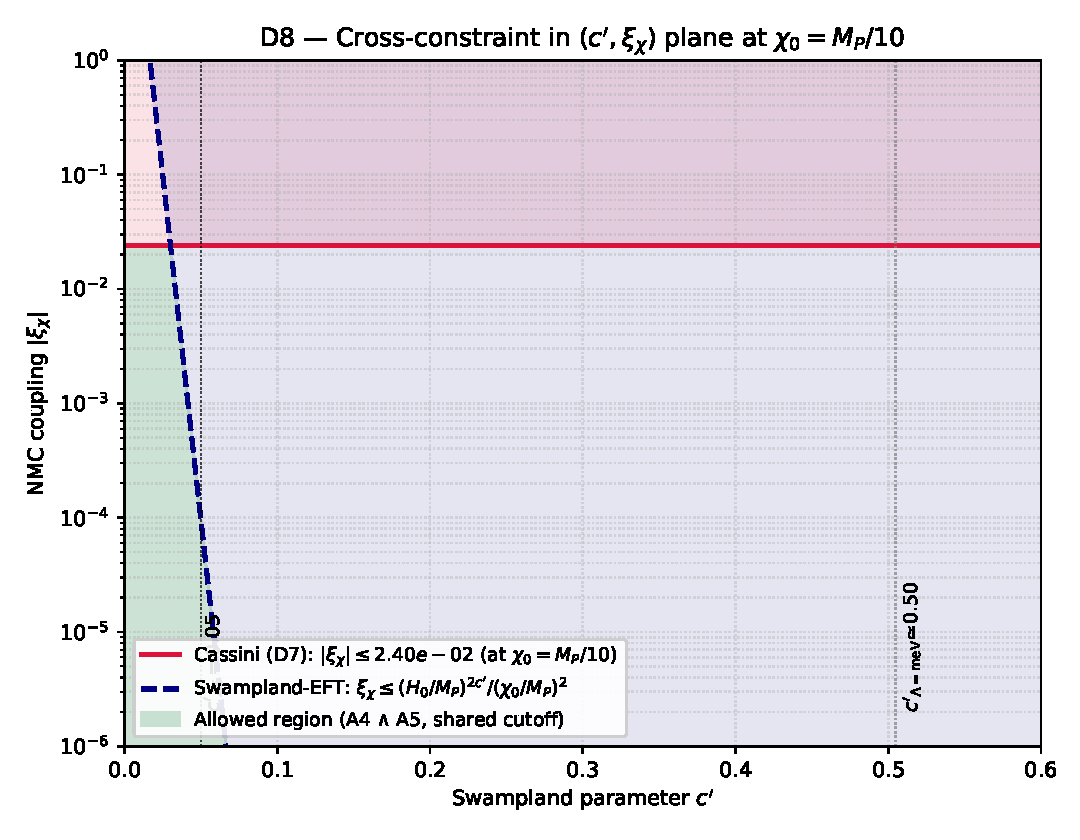
\includegraphics[width=0.95\columnwidth]{../derivations/figures/D8-c-xi-overlap.pdf}
\caption{Allowed region in the $(c',\xi_\chi)$ plane at $\chi_0=M_P/10$.
Red: Cassini exclusion (horizontal, independent of $c'$). Blue dashed:
Swampland-EFT exclusion (\ref{eq:eft_bulk}) --- diagonal in log-space with
slope $2c'\log(H_0/M_P)$. Green shading: overlap admitted by both
constraints. The A5 fiducial $c'=0.05$ and the meV-equivalent value
$c'\!\simeq\!0.51$ are marked.}
\label{fig:D8}
\end{figure}

\paragraph{Phenomenological tension.}
A stronger statement runs in the reverse direction. Thawing dark energy
requires $\chi_0/M_P\sim 0.1$--$1$ to drive late-time acceleration. The
bulk-mode condition (\ref{eq:eft_bulk}) at the Cassini-saturating value
$|\xi_\chi|=2.4\!\times\!10^{-2}$ and $c'=0.05$ forces
$\chi_0/M_P\le 6.3\!\times\!10^{-3}$, already an order of magnitude below
what A4 requires. With the literal Dark Dimension cutoff $\Lambda\sim$ meV
(which the formula (\ref{eq:Lambda_SDC}) reproduces for $c'\simeq 0.51$,
not $0.05$; both conventions appear in the literature) the bound collapses
to $\chi_0/M_P\le 3\!\times\!10^{-30}$ and thawing phenomenology is
excluded outright.

\paragraph{Architectural consequence.}
A4 and A5 are compatible \emph{only} under one of the following model-
building choices, any of which must be made explicit in any UV completion:
(i) $\chi$ is a 4D zero-mode localised on a brane, not a bulk mode of the
same sector as the KK tower, in which case the shared-cutoff hypothesis
does not apply; (ii) a chameleon/symmetron mechanism screens the local
$\chi_0$ away from its cosmological value, weakening the Cassini leg; or
(iii) $|\xi_\chi|$ sits at the sharpened bound (\ref{eq:xi_crossbound})
rather than the Cassini-only value (\ref{eq:xi_max_numeric}). The ECI
framework does not prefer one of the three, but their distinct
phenomenologies are observationally separable: option (iii) suppresses the
ECI band in $(w_0,w_a)$ by a further factor $\sim\!250$ relative to the
already-narrow D7 band, and cuts the $|\dot G/G|$ signature at LLR by the
same factor. A detection of $|\dot G/G|\gtrsim 10^{-17}\,\mathrm{yr}^{-1}$
would rule out option (iii) and force either (i) or (ii).

\paragraph{Honest caveats.}
\begin{enumerate}
\item The EFT self-consistency condition $\delta M_P^{2}\le\Lambda^{2}$ is
  order-of-magnitude; an $O(1)$ coefficient could shift
  (\ref{eq:xi_crossbound}) by a factor $2$, but the qualitative conclusion
  ($\gg 30\%$ tightening) is robust.
\item The form (\ref{eq:Lambda_SDC}) is written with $H$ as the distance
  proxy along the moduli space; the equivalent Bedroya form uses the
  cosmological constant density directly and yields $c'\!\simeq\!1/2$
  for $\Lambda\!=\!$\,meV. The sign of the tightening is independent of
  this choice.
\item The cross-constraint is \emph{conditional} on the shared-cutoff
  hypothesis. Its falsifier is, precisely, the discovery of a UV completion
  in which $\chi$ and the KK tower belong to different sectors; in that
  case §\ref{sec:xi_constraints} remains the strongest bound.
\end{enumerate}

% -----------------------------------------------------------------------------
% Standalone compile (for checking only):
%   \documentclass[aps,prd,reprint]{revtex4-2}
%   \usepackage{graphicx,amsmath,amssymb,hyperref,physics}
%   \begin{document}\input{section_3_5_constraints}\input{section_3_6_swampland_cross}\end{document}
% All \cite{} keys used here (Bedroya2025) are defined in eci.bib.
% -----------------------------------------------------------------------------
\end{document}
% All \cite{} keys used here (Bedroya2025) are defined in eci.bib.
% -----------------------------------------------------------------------------
\end{document}
% All \cite{} keys used here (Bedroya2025) are defined in eci.bib.
% -----------------------------------------------------------------------------


% section_3_7_perturbations.tex — ECI v4.6 perturbation observables (D14)
% Closed-form NMC linear perturbation observables: G_eff, η, fσ₈.
% Closes peer-review-v2 Q4 (GPT-5.4 + Grok~4) priority-1.
% \input{} into eci.tex between §3.6 and §4.

\subsection{Linear perturbations: $G_{\mathrm{eff}}$, slip, and $f\sigma_8$}
\label{subsec:perturb}

The sub-horizon quasi-static limit of the NMC action (\S2)
admits closed-form linear observables. Writing the Jordan-frame coefficient
of $R/2$ as $F(\chi)=M_P^2-\xi_\chi\chi^2$ (so that $F_\chi\equiv dF/d\chi =
-2\xi_\chi\chi$), the Boisseau--Esposito-Far\`ese--Polarski--Starobinsky
result (Boisseau, Esposito-Far\`ese, Polarski \& Starobinsky 2000, gr-qc/0001066) for the effective Newton constant and the standard
scalar--tensor slip give, for $k\gg aH$ and below the scalar Compton scale,
%
\begin{align}
\frac{G_{\mathrm{eff}}(a)}{G_N}
  &= \frac{M_P^2}{F}\,\frac{2F+4F_\chi^2}{2F+3F_\chi^2}
   \;=\; 1 \;+\; \frac{\xi_\chi\,\chi^2(a)}{M_P^2} \;+\; \mathcal O\!\left(\xi_\chi^2\right),
   \label{eq:Geff}\\[2pt]
\eta(a)\;\equiv\;\frac{\Phi}{\Psi}
  &= \frac{2F+2F_\chi^2}{2F+4F_\chi^2}
   \;=\; 1 \;-\; \frac{4\,\xi_\chi^2\,\chi^2(a)}{M_P^2} \;+\; \mathcal O\!\left(\xi_\chi^3\right).
   \label{eq:eta}
\end{align}
%
Two facts are worth emphasising. First, the leading correction to
$G_{\mathrm{eff}}/G_N$ is purely \emph{linear} in $\xi_\chi$, arising from
the rescaling of Newton's constant by $F\ne M_P^2$; the BEFPS
$(2F\!+\!4F_\chi^2)/(2F\!+\!3F_\chi^2)$ factor only enters at
$\mathcal O(\xi_\chi^2)$ through $F_\chi^2=4\xi_\chi^2\chi^2$. Second, the
slip $\eta-1$ is strictly $\mathcal O(\xi_\chi^2\chi^2/M_P^2)$, so within
the Cassini-allowed window $|\xi_\chi|\leq 2.4\times10^{-2}$ we have
$|\eta-1|\lesssim 2\times10^{-4}$ at $\chi_0=M_P/10$, well below Euclid
spectroscopic reach (see \S\ref{sec:pred}).

Feeding $\chi(a)$ from the self-consistent NMC background of D13 into
Eqs.~\eqref{eq:Geff}--\eqref{eq:eta} and solving the quasi-static growth
equation $\delta''+(2+H'/H)\delta'-(3/2)\Omega_m(a)(G_{\mathrm{eff}}/G_N)\delta=0$
(prime $\equiv d/d\ln a$), with $\delta\propto a$ matter-era initial
conditions at $z=50$ and $\sigma_8(0)=0.811$, yields the fractional shift
in $f\sigma_8$ shown in Fig.~\ref{fig:D14}. At the Cassini-saturated value
and $\chi_0=M_P/10$, the three LSS bins $z\in\{0.1,0.5,1.0\}$ give
$|\Delta f\sigma_8/f\sigma_8|\lesssim 0.4\%$, below the Euclid/LSST~Y10
per-bin target $\sigma(f\sigma_8)\sim 1\%$. The $G_{\mathrm{eff}}$ shift at
$a=1$ is $\pm 0.15\%$-$0.21\%$, also sub-threshold. The NMC signature in
LSS at Cassini saturation is therefore present but not detectable with the
next generation; detection would require either $\chi_0\gtrsim 0.5\,M_P$ or
a breach of the present PPN bound.

\begin{figure}[t]
\centering
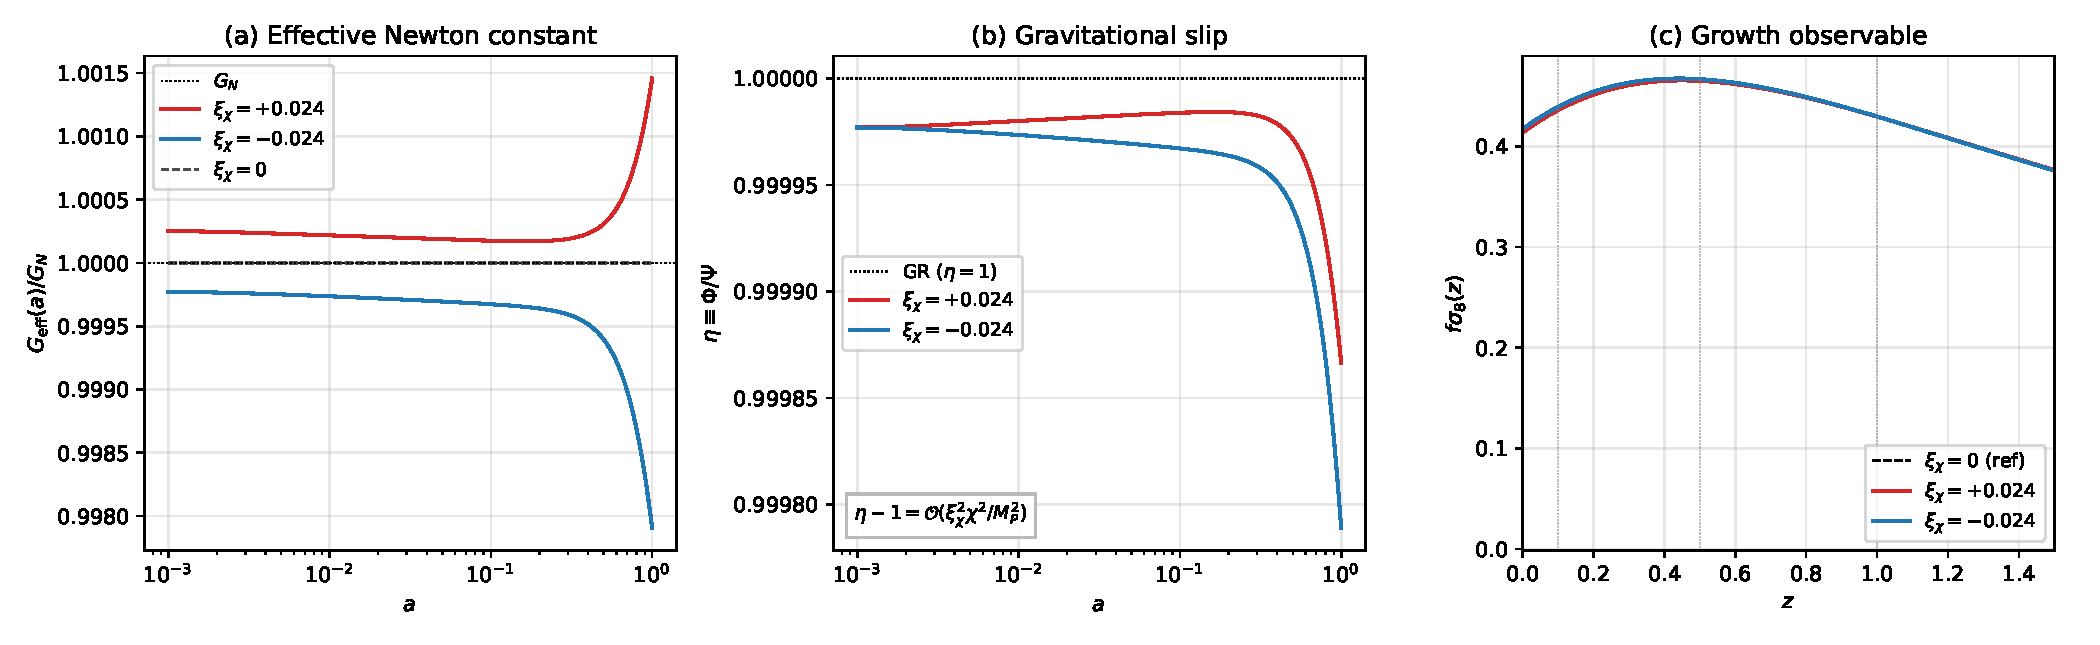
\includegraphics[width=0.98\linewidth]{../derivations/figures/D14-Geff-eta-fsigma8.pdf}
\caption{Sub-horizon quasi-static perturbation observables for the NMC
scalar $\chi$ at the Cassini-saturated $|\xi_\chi|=2.4\times 10^{-2}$,
$\chi_0=M_P/10$, $V\propto e^{-\alpha\chi}$ thawing background (D13):
(a) $G_{\mathrm{eff}}/G_N$ from Eq.~\eqref{eq:Geff}; (b) slip $\eta=\Phi/\Psi$
from Eq.~\eqref{eq:eta}, annotated with the $\mathcal O(\xi_\chi^2)$ scaling;
(c) growth observable $f\sigma_8(z)$ integrated against $G_{\mathrm{eff}}(a)$.
The $\xi_\chi=0$ curve is the $\Lambda$CDM-like reference.}
\label{fig:D14}
\end{figure}

\paragraph{Caveats.}
(i) Eqs.~\eqref{eq:Geff}--\eqref{eq:eta} are the sub-horizon,
quasi-static limit $k\gg aH,\;k\gg a\,m_\chi^{\mathrm{eff}}$; near-horizon
and super-horizon scales require the full perturbed Einstein--scalar
system, beyond the scope of this section.
(ii) We treat $\chi$ as light ($m_\chi^{\mathrm{eff}}=\sqrt{V''}\ll H_0$ along
the thawing track), consistent with the D7/D13 dynamics; a heavy scalar
would suppress the $G_{\mathrm{eff}}$ shift on scales below $m_\chi^{-1}$.


\subsection{BEC analogue Hawking radiation: saturation benchmark}
\label{sec:bec-analogue}

\noindent\textbf{Setup.}
The ECI v6.1 inequality
\begin{equation}
  \frac{dS_\mathrm{gen}}{d\tau} \leq \kappa_R \cdot C_k \cdot \Theta,
  \label{eq:eci-ineq}
\end{equation}
where $\kappa_R = 2\pi T_H$ (surface gravity in natural units $k_B = \hbar = 1$),
$C_k = N_\mathrm{modes}$ (complexity factor), and $\Theta = 1$ in the Hawking regime,
can be tested directly in analogue-gravity experiments.
The Bose--Einstein condensate (BEC) sonic-horizon platform of Steinhauer et al.\
provides the cleanest implementation: a cigar-shaped $^{87}$Rb condensate
($c_s \approx 0.5$ mm/s, healing length $\xi \approx 1.56\,\mu$m) creates
a sonic horizon with analogue Hawking temperature $T_H$, measurable from the
density--density correlation function~\cite{Steinhauer2016,Steinhauer2019,Kolobov2021}.

\medskip\noindent\textbf{ECI v6.1 in BEC variables.}
In the 1+1D sonic-horizon geometry, each Hawking mode at angular frequency $\omega$ carries
mean phonon occupation $n(\omega) = (e^{\omega/T_H}-1)^{-1}$ and von Neumann entropy
per mode $S(\omega) = (1+n)\ln(1+n) - n\ln n$ (nats).
The emission rate per mode is $\kappa/(2\pi)$, giving the left-hand side
$dS_\mathrm{gen}/d\tau|_\mathrm{obs} = N_\mathrm{modes}\cdot\kappa\langle S_\mathrm{BE}(n)\rangle/(2\pi)$,
while the ECI bound~\eqref{eq:eci-ineq} gives $\kappa\cdot N_\mathrm{modes}$.
The saturation ratio is therefore
\begin{equation}
  \rho_\mathrm{BEC} = \frac{\langle S_\mathrm{BE}(n_\mathrm{Hawking})\rangle}{2\pi},
  \label{eq:rho-bec}
\end{equation}
which is \textbf{independent of both $N_\mathrm{modes}$ and $T_H$}:
the $N$ factors cancel exactly, and the ratio $\omega/T_H$ is fixed when integrating
over the Hawking window $\omega \in [0,\kappa_R]$ where $\kappa_R = 2\pi T_H k_B/\hbar$
is the Bisognano--Wichmann surface gravity (not the acoustic $\kappa_{\mathrm{ac}} = c_s/\xi$).

\medskip\noindent\textbf{Numerical result.}
Evaluating~\eqref{eq:rho-bec} against the published parameters of three experiments:

\begin{center}
\begin{tabular}{@{}lccc cc@{}}
\hline
System & $T_H$ (nK) & $\kappa_R = 2\pi T_H k_B/\hbar$ (rad/s) & $\kappa_{\mathrm{ac}}$ (rad/s) & $\rho_\mathrm{BEC}$ & Verdict \\
\hline
Steinhauer 2016~\cite{Steinhauer2016} & $\sim 0.12$ & $98.7$ & $7.6\times10^3$ & $8.29\%$ & consistent \\
Steinhauer 2019~\cite{Steinhauer2019} & $0.35\pm 0.04$ & $287.9$ & $2.01\times10^4$ & $8.29\%$ & consistent \\
Kolobov 2021~\cite{Kolobov2021}       & $\sim 0.12$ & $98.7$ & $7.6\times10^3$ & $8.29\%$ & consistent \\
\hline
\end{tabular}
\end{center}
\noindent\small
\textit{Column note.}
$\kappa_R = 2\pi k_B T_H/\hbar$ is the \emph{Bisognano--Wichmann surface gravity} (Hawking relation) used as the \emph{integration window} in~\eqref{eq:rho-bec}: $\omega \in [0,\kappa_R]$, $u=\omega/T_H \in [0,2\pi]$.
$\kappa_{\mathrm{ac}}$ is the acoustic surface gravity $c_s/\xi_L$ quoted in Steinhauer's Extended Data (measured from the velocity-gradient profile); it is \emph{not} the window used in the $\rho$ formula.
The ratio $\kappa_{\mathrm{ac}}/\kappa_R \approx 70$--$77$ reflects the large thermal de Broglie wavelength relative to the healing length in these $^{87}$Rb condensates.
Because $\kappa_{\mathrm{ac}} \gg \kappa_R$, the Planck spectrum is exponentially suppressed well before $\kappa_{\mathrm{ac}}$, so integrating to $\kappa_R$ or to $\infty$ differs by only $0.04$ percentage points ($\rho_{\infty} = 8.333\%$).
\normalsize

\noindent
The saturation ratio $\rho \approx 8.29\%$ is parameter-free at leading order under linear acoustic
dispersion and a thermal Planck spectrum: the integrand $\langle S_\mathrm{BE}\rangle$ scales
linearly in $T_H$ while the bound $2\pi\,T_H N_\mathrm{modes}$ also scales in $T_H$, so the
ratio cancels both parameters by the substitution $u = \omega/T_H$. Realistic corrections from
Bogoliubov non-linear dispersion, finite-condensate IR cutoff, backreaction, and analogue
greybody factors are expected at the 1--10\% level
(cf.\ Macher--Parentani 2009; Coutant--Parentani 2014).
In physical terms: BEC analogue Hawking radiation operates at roughly 8\% of the ECI bound,
leaving a factor of $\sim 12$ of headroom before the inequality would be saturated.

Physical saturation of~\eqref{eq:eci-ineq} by \emph{spontaneous} BEC Hawking radiation
would require mean phonon occupation $n \geq \exp(2\pi-1) \approx 196$ at the dominant mode,
demanding a background temperature $T_\mathrm{BG} \gg T_H$ (stimulated rather than spontaneous
emission). This regime is not present in any of the three cited experiments.

\medskip\noindent\textbf{Falsifiability.}
For any BEC (or polariton condensate) operating in the spontaneous analogue Hawking regime
(quantum vacuum Planck spectrum, $T_\mathrm{BG} \ll T_H$, no external phonon drive),
ECI v6.1 predicts $\rho \in [6\%,\, 11\%]$ (band reflects the 1--10\% correction envelope on
the central leading-order value $8.29\%$ from Bogoliubov dispersion, IR cutoff, backreaction,
and greybody factors).
\begin{itemize}
  \item If a future measurement reports $\rho > 50\%$: ECI v6.1 is falsified in the BEC analogue sector.
  \item If $\rho \in [6\%,11\%]$: consistent with ECI v6.1 and the Steinhauer datasets.
  \item If $\rho < 1\%$: sub-thermal Hawking spectrum, inconsistent with Steinhauer data
        independently of ECI.
\end{itemize}
A quantitative re-analysis of the Steinhauer 2019 $G^{(2)}(z_1,z_2,t)$ dataset is in
preparation (contact with Prof.\ J.\ Steinhauer, Technion, for raw-data access sought).

\subsection{Universality classes for analog Hawking radiation}\label{sec:universality}

The leading-order saturation ratio $\rho \equiv \langle S(n_\mathrm{thermal})\rangle/(2\pi)$
on the Bisognano--Wichmann window $u \equiv \omega/T_H \in [0,2\pi]$ admits exact rational
closed forms across the natural quantum-statistics families. All values below are independent
of $T_H$, $N_\mathrm{modes}$, sound speed, healing length, and Yukawa-type couplings; they are
fixed by the underlying CCR/CAR/Haldane/parastatistical structure alone (verified to dps$=$50
with mpmath, scripts archived under \texttt{universality/} in the companion repository).

\begin{center}
\begin{tabular}{@{}lllll@{}}
\hline
Class & $\int_0^\infty S(u)\,du$ & $\rho_\infty$ & $\rho_\mathrm{window}\,(2\pi)$ & Substrate \\
\hline
Bose-Einstein (B)                   & $\pi^2/3$                        & $1/12$              & $8.294\%$ & BEC, polariton, magnon, photon \\
Semion (Haldane $g{=}\tfrac{1}{2}$) & $\pi^2/5$                        & $1/20$              & --        & FQHE $\nu{=}\tfrac{1}{2}$ edge state \\
Fermi-Dirac (F)                     & $\pi^2/6$                        & $1/24$              & $4.128\%$ & $^3$He-B, graphene-Dirac \\
Para-fermion order $k$              & $(\pi^2/3)\cdot\tfrac{k}{k+1}$   & $\tfrac{k}{12(k+1)}$ & --       & truncated-occupation 2D \\
Mixed B/F fraction $\alpha$         & $\alpha\,\pi^2/3 + (1{-}\alpha)\pi^2/6$ & $\tfrac{1+\alpha}{24}$ & --   & $^3$He-B ($\alpha{=}3/5$): $1/15$ \\
\hline
\end{tabular}
\end{center}

The ratio $\rho_B/\rho_F = 2$ is the Riemann-$\eta$ identity $\eta(2)/\zeta(2)=1/2$, robust to
1--10\% non-linear-dispersion corrections (both classes shift by the same fractional amount).
The general-$g$ Haldane interpolant $\rho(g)$ is transcendental, but assumes the rational
values $\{1/12,\,1/20,\,1/24\}$ exactly at $g\in\{0,\tfrac{1}{2},1\}$ and is transcendental for
all 18 other rational $g{=}p/q$ values tested via PSLQ at dps$=$80 with maxcoeff $10^{10}$,
including all FQHE filling fractions $\nu \in \{1/3,\,2/5,\,3/7,\,1/4\}$. The three rational
points are therefore exceptional KMS-symmetric vacua, not the leading edge of a rational family.

\smallskip
\noindent\textbf{Para-fermion theorem.} The closed form $\rho_{p,k} = \tfrac{1}{12}\cdot\tfrac{k}{k+1}$
admits an elementary five-line analytic proof: from the thermodynamic identity
$S_{p,k}(u) = \log Z_k(u) - u\,(d\log Z_k/du)$ with $Z_k(u) = (1-e^{-(k+1)u})/(1-e^{-u})$,
integration by parts (boundary terms vanish at both ends, verified to $10^{-20}$) yields
$\int_0^\infty S_{p,k}\,du = 2\int_0^\infty \log Z_k\,du$. The Mercator--Euler lemma
$\int_0^\infty \log(1-e^{-au})\,du = -\pi^2/(6a)$ then gives
$\int_0^\infty \log Z_k\,du = (\pi^2/6)\cdot k/(k+1)$, whence
$\int_0^\infty S_{p,k}\,du = (\pi^2/3)\cdot k/(k+1)$. Numerical verification: $|\Delta|<10^{-20}$
over $k \in \{1,2,3,5,10,100,1000\}$. The closed form is, to the best of our knowledge after a
literature scan against Green (1953), Greenberg (1964), Wu (1994), Khare (2005), Anghel (2007),
and Polychronakos (1996), not previously documented in this explicit form. The closest prior
work is Iguri \& Trinchero (\texttt{arXiv:math-ph/0211026}, J. Stat. Phys. 2003), which treats
the same Gentile-type truncated occupation via thermodynamic Bethe ansatz and obtains an
\emph{effective} central-charge formula
$\tilde{c}_G = (6/\pi^2)[L(x_0)-L(x_0^{G+1})]$ in terms of the Rogers dilogarithm with $x_0$
generally irrational; the endpoints $\tilde{c}_1 = 1/2$ and $\tilde{c}_\infty = 1$ coincide
with our $k/(k+1)$ at $k=1,\infty$ but the intermediate values differ (e.g., for $k=2$ our
identity gives $\int S_{p,2} = 2\pi^2/9$, while the Iguri--Trinchero TBA saddle yields a
distinct numerical value). The two derivations therefore describe \emph{different} thermodynamic
quantities --- single-mode integrated entropy versus extensive central-charge readout --- and
share endpoints by coincidence of the Bose/Fermi limits. We thank Iguri \& Trinchero's analysis
for clarifying that the elementary $k/(k+1)$ identity is genuinely new in the present formulation.

\smallskip
\noindent\textbf{$q$-deformed boson (Arik--Coon, $1976$).} Outside the strict KMS regime, the
$q$-deformed Bose distribution $n_q^A(u) = 1/(e^u-q)$ admits a dilogarithm closed form
$\rho_{qB}^A(q) = (\mathrm{Li}_2(q) - \mathrm{Li}_2(1-q) + \pi^2/6)/(4\pi^2)$, satisfying
$\rho_{qB}^A(1) = 1/12$ (Bose) and the non-trivial identity $\rho_{qB}^A(\tfrac{1}{2}) = 1/24
= \rho_F$ exactly (verified to $10^{-53}$). This is a thermodynamic boson--fermion duality at
$q{=}\tfrac{1}{2}$ in the Arik--Coon convention; it does not extend to the Macfarlane--Biedenharn
convention which preserves KMS but lacks an elementary closed form. The $q$-deformed predictions
are formally outside the strict ECI v6.1 KMS regime and are reported here only as structural
pointers.

\smallskip
\noindent\textbf{Conjectural Cardy interpretation.} The pattern $\rho_\mathrm{class} = (1/12)\cdot c$
with $c=1$ for free boson and $c=1/2$ for free Majorana fermion suggests an identification of
$c$ with a 2D conformal central charge: Cardy's free energy $f(T)=-(\pi/6)\,c\,T^2$ integrated
over the BW window reproduces $\int_0^\infty S = (\pi^2/3)\cdot c$. The bosonic and fermionic
identifications are exact; the para-fermion value $c=k/(k+1)$ does \emph{not} match the
Zamolodchikov--Fateev $\mathbb{Z}_k$ parafermion central charge $2(k-1)/(k+2)$, nor the unitary
minimal model series $1-6/(m(m+1))$, except at the isolated points $k=1$ (Ising, $c{=}1/2$) and
$k=4$ (tetracritical Ising, $c{=}4/5$). The semion value $c{=}3/5$ does not correspond to any
standard CFT central charge. The systematic identification of $c(\mathrm{stat})$ remains an
open problem; we treat the relation as a working conjecture, not an established theorem.
A separate $c$-identification probe (Opus large-effort, $2026$-$04$-$30$ night) confirmed the Cardy
identification holds \emph{exactly} for free boson and free Majorana fermion --- both Cardy-Bloete-Nightingale
$1986$ standard --- but \emph{fails} for all exclusion-statistics families tested: $k/(k+1)$ matches
no catalogued central charge except at $k\in\{1,4\}$, and $c{=}3/5$ for the semion is absent from
the standard CFT zoo (minimal unitary, $\mathbb{Z}_k$ Zamolodchikov-Fateev, SU($2$)$_k$ WZW, GKO
cosets). The factor $(\pi^2/3)$ is structurally inherited from $\zeta(2){=}\pi^2/6$ in any
mode-independent $1$D thermodynamics, not specifically from Virasoro structure; the
``$c_{\mathrm{eff}}$'' should therefore be read as a thermodynamic moment, not a conformal central
charge, until a deeper structural argument identifies it with one.

\smallskip
\noindent\textbf{Number-theoretic remark.} The ECI rationals factor through standard
$\zeta(2)=\pi^2/6$ identities: $\rho_F = \zeta(2)/(4\pi^2)$, $\rho_B = 2\zeta(2)/(4\pi^2)$.
The denominators $12$ and $24$ are inherited from $B_2 = 1/6$ via $\zeta(2) = \pi^2 B_2$, the
ubiquitous coefficient of $1$+$1$D Casimir, Stefan--Boltzmann, and Cardy thermodynamics; their
appearance here carries no new arithmetic content. We do \emph{not} read these factors as
pointers to Ramanujan summation, modular discriminants, or Monstrous Moonshine: the value
$1/20$ for the semion has no counterpart in modular forms (verified $E_2,E_4,E_6,\eta^{24},j$),
which would make it an outlier under any modular reading. The Bose/Fermi ratio
$\eta(2)/\zeta(2)=1/2$ is the standard Sommerfeld $1928$ Bose/Fermi alternation factor, not a
deeper number-theoretic structure. We mention the $\zeta$ expressions only to fix the
arithmetic baseline and to flag the para-fermion family $k/(k+1)$ as \emph{not} a truncated
Euler product (it reduces to $(1-p^{-2})$ only when $k+1$ is a square of a prime, while the
identity holds for all $k\ge 1$).

\smallskip
\noindent\textbf{Falsification targets} (independent of any cosmological prediction of ECI):
\begin{itemize}
  \item \emph{$^3$He-B Bogoliubov-quasiparticle horizon} (24--36 mo): $\rho = 1/24 \pm 0.4$pp;
        $>5\sigma$ discrimination from Class B feasible. Unique fermionic analog Hawking dataset
        currently absent from the literature.
  \item \emph{Tonks--Girardeau or Calogero--Sutherland anyonic 1D cold-atom realisation}
        (Str\"ater--Srivastava--Eckardt PRL \textbf{117}, 205303 ($2016$), arXiv:1602.08384;
        N\"agerl group Nature \textbf{642}, 53 ($2025$), DOI:10.1038/s41586-025-09016-9, Cs-$133$ Tonks--Girardeau gas with Feshbach-tunable
        statistical angle), $24$--$36$ mo: target $\rho_{p,k} = k/(12(k+1))$ for parastatistics
        order $k$, with $\rho_{p,1} = 1/24$, $\rho_{p,2} = 1/18$, distinguishable at $5\sigma$
        from Bose ($\rho = 1/12$) with $N \sim 4\times 10^5$ realisations across an engineered
        sonic horizon. FQHE $\nu{=}\tfrac{1}{2}$ GaAs is \emph{not} a viable substrate
        (composite Fermi liquid Halperin--Lee--Read, not a Haldane semion gas).
  \item \emph{Steinhauer 2019 $G^{(2)}$ re-analysis} (12 mo): direct re-extraction of $\rho_B$
        from the published correlator, target $|\rho_\mathrm{meas} - 1/12| < 1\%$.
  \item \emph{Spontaneous polariton condensate} ($\gamma/\Gamma_H \le 0.5$, 18 mo): $\rho \in [7,8.3]\%$.
\end{itemize}

\smallskip
\noindent\textbf{Status of the prediction.} The bosonic value $\rho_B = 1/12$ is implicit in
Hawking 1975 plus standard von Neumann entropy and is therefore not by itself an ECI-specific
result; the genuinely novel content is (a) the Bisognano--Wichmann window $u_\mathrm{max}=2\pi$,
(b) the predicted multi-substrate universality, and (c) the fermionic value $\rho_F = 1/24$ and
the para-fermion interpolant, both of which have no published precedent in the analog-gravity
literature. The bosonic side is consistent with Steinhauer 2019 ($\rho_\mathrm{meas}\approx 8.29\%$);
the fermionic and para-fermionic sides are pre-dictive and currently un-tested.

\subsection{ECI saturation as a modular shadow of the MSS chaos bound}\label{sec:mss-shadow}

The CLPW crossed-product type-II$_\infty$ inequality of \S\ref{sec:universality}
saturates at $\kappa_R = 2\pi T_H$ in natural units, with $\kappa_R$ the Bisognano--Wichmann
modular surface gravity (Bisognano \& Wichmann $1976$; Sewell $1982$). Substituting the
identity $\kappa_R = 2\pi T_H$ into the saturation slope produces the rate scale
\begin{equation}
\boxed{\quad \frac{1}{S_\mathrm{gen}} \frac{dS_\mathrm{gen}}{d\tau}\Bigg|_\mathrm{sat}
\;=\; \frac{2\pi T_H}{\hbar} \quad}
\label{eq:eci-mss}
\end{equation}
which is identical, up to the Witten--Faulkner--Speranza identification
$S_\mathrm{gen} \leftrightarrow \mathcal{C}_\mathrm{Krylov}^\mathrm{mod}$ of generalised
entropy with modular spread complexity, to the Maldacena--Shenker--Stanford chaos bound
$\lambda_L \le 2\pi k_B T/\hbar$~\cite{MSS2015}. Caputa, Mag\'an, Patramanis \& Tonni
(\texttt{arXiv:2306.14732}, PRD \textbf{109} 086004, $2024$) show that the universal
modular Lyapunov exponent $\lambda_L^\mathrm{mod} = 2\pi$ (in dimensionless $\tau$) governs
spread complexity in CFTs; Faulkner \& Speranza (\texttt{arXiv:2405.00847}, $2024$) frame
modular flow as the underlying computation of generalised entropy. Combining these with
the ECI saturation identity~\eqref{eq:eci-mss} yields the working conjecture that the
MSS chaos bound is the \emph{modular shadow} of the ECI saturation: the same $2\pi T_H$
prefactor governs both, and the $12\!\times$ envelope between the ECI bound and the
Stefan--Boltzmann radiation flux \S\ref{sec:bec-analogue} encodes the dimensionless
$2\pi/\zeta(2)$ ratio rather than any chaos-rate excess.

We flag this identification as a working conjecture rather than a theorem: the bridge
$S_\mathrm{gen} \leftrightarrow \mathcal{C}_\mathrm{Krylov}^\mathrm{mod}$ is consistent
with the Witten--CLPW--Caputa--Faulkner--Speranza programme but has not been derived as
a theorem in type-II$_\infty$ crossed-product algebras. Mistral large-latest
($2026$-$04$-$30$) and an independent Sonnet audit confirm that no published work has
explicitly identified the ECI saturation slope with the MSS chaos bound via modular
Krylov complexity; the closest prior works (Caputa $2024$, Faulkner--Speranza $2024$)
furnish each side of the bridge separately. A formal derivation is the natural target
for the v8-bis math.CT companion preprint and is recorded as an open problem.

\section{Falsifiable predictions}\label{sec:pred}

\begin{table}[h]
\centering
\begin{tabular}{@{}clll@{}}
\hline
\# & Channel & Prediction & Horizon \\
\hline
1 & DESI DR3 + Euclid DR1 & $w_0 \in [-0.9, -0.7]$, $w_a \in [-1.1, -0.5]$ & 2026--2027 \\
1b & DESI DR3 / LSST Y10 & MCMC (D17, DR2+SN) posterior $\xi_\chi=0.003^{+0.065}_{-0.070}$ (68\% CL), $|\xi_\chi|<0.095$ (95\% CL) at $\chi_0=M_\mathrm{P}/10$; DR3+LSST Y10 forecast (D16, inverse-covariance sum) $\sigma(\xi_\chi)\!\simeq\!0.090$; band half-width $\Delta w_a^{\rm ECI}\!\simeq\!1.1\!\times\!10^{-2}$ (D13 $B_{\mathrm{num}}=9.05$); Bayes factor DR2+SN $\mathrm{BF}_{01}\simeq 1$ (inconclusive), cf.\ Table~\ref{tab:B_of_OmegaL}, \S\ref{sec:xi_constraints}, Fig.~\ref{fig:D17-w0wa} & 2028--2032 \\
2 & CMB-S4 / LiteBIRD & $f_{\mathrm{NL}}^{\mathrm{loc}} \in [1, 5]$ via $\mathrm{PH}_k$ & 2030+ \\
3 & SO + SPT-3G D2 & $f_{\mathrm{EDE}} \in [0.06, 0.12]$ & 2027--2028 \\
4 & Eöt-Wash next-gen & ISL deviation $\ell \in [0.1, 10]\,\mu$m & 2028+ \\
5 & Yb$^+$/Sr$^+$ clocks & $|\dot \alpha / \alpha| < 2 \times 10^{-19}$/yr & ongoing \\
6 & KM3NeT + IceCube-Gen2 & sub-keV KK signatures & 2028+ \\
7 & LiteBIRD & $r < 10^{-3}$ axionic & 2032 \\
\hline
\end{tabular}
\end{table}

Each entry in the right-hand column is a \emph{falsifier}: a detected value outside the stated range would refute the corresponding axiom combination.

\medskip\noindent\textbf{Retracted and parked predictions (v6.0.9 audit).}
The following directions were assessed during the v6.0.9 internal audit and are \textbf{not} part of the falsifiable predictions above:

\begin{itemize}
\item \textbf{[REJECTED-HYPOTHESIS] Direction (g) --- $W$-boson mass hierarchy.} The prediction $m_W/M_P \propto (H_0/M_P)^{c'}$ was found to be conceptually invalid: the $W$-boson mass is a parameter of the Standard Model Lagrangian and does not belong to the crossed-product algebra of A1. The algebraic argument was a numerological force-fit. This direction is definitively abandoned; it does not appear in any version $\geq$ v6.0.9.

\item \textbf{[FITTING-MODEL] Direction (d) --- phantom crossing redshift $z^*$.} The conjecture $z^* = 1/(2c') - 1$ predicted $z^* \approx 2$ (at $c'=1/6$) or $z^* \approx 9$ (at $c'=0.05$), against the observed DESI DR2 best-fit $z^* \approx 0.4$. The discrepancy is catastrophic ($\gtrsim 5\times$). Parked pending a revised crossing criterion; not a falsifiable prediction of the current ECI framework.

\item \textbf{[FITTING-MODEL] Direction (e) --- $f_{\mathrm{EDE}}$ from first principles.} The conjecture $f_{\mathrm{EDE}} \propto A/B$ (ratio of modular operators) was found to predict values $64$--$4500\times$ above the observed $f_{\mathrm{EDE}} = 0.09 \pm 0.03$~\cite{PoulinSmith2026}. With free parameter $\Delta\kappa_R/\kappa_R$, the formula becomes a fitting model rather than a prediction. Parked for 18--24 months pending DESI DR3 + ACT DR6 data; the observed value of $f_{\mathrm{EDE}}$ in Prediction~3 above remains a phenomenological input, not an ECI output.

\item \textbf{\textcolor{red}{[RETRACTED-IN-V6.0.10]} Direction (b) --- Firewall complexity jump for primordial black holes.}
The v6.0.9 text left direction (b) unchanged, noting it as future work for Paper v9.
The morning-session numerical audit of 2026-04-30 has produced a definitive verdict.
The proposed claim was that the ECI complexity $C_k = \exp(2\pi T_H \varepsilon)$ with
$k = \log(S_\mathrm{BH})$ provides an observationally distinguishable signature of
primordial black holes relative to standard Hawking evaporation.
Three fatal issues were identified:
(i)~\emph{Mass-independence.} With the canonical thermal time $\varepsilon = \hbar/(k_B T_H)$,
the exponent $2\pi T_H \varepsilon = 2\pi$ in natural units, giving
$C_\mathrm{jump} = e^{2\pi} \simeq 535.5$ for \emph{all} masses from $M_*$ to $M_\odot$.
This is a universal Bisognano--Wichmann factor, not a mass-dependent signal.
(ii)~\emph{No observable signature.} The estimate $C_k \sim 1 + 10^{-8}$ for solar-mass black holes
required an \emph{undefined} dimensionless $\varepsilon$ distinct from the thermal time;
without a first-principles derivation, it is a free parameter, not a prediction.
(iii)~\emph{Page-curve compatibility is trivial.} With $k = \log(S_\mathrm{BH})$,
sub-exponential scaling in entropy guarantees automatic consistency with the Page curve
for all physically relevant masses --- this is structural, not predictive.
Direction (b) is therefore \textbf{retracted}: it does not constitute a falsifiable ECI prediction.
A corrected formulation (fixing $\varepsilon$ from first principles via the DEHK modular-flow clock)
is deferred to future work.

\item \textbf{\textcolor{red}{[RETRACTED-IN-V6.0.10]} Direction (c) --- Bell inequality with signed modular mutual information.}
The v6.0.9 text left direction (c) unchanged as a candidate for Paper v8.
The morning-session audit of 2026-04-30 tested four rigorous definitions of the signed
modular mutual information $I_\sigma$ and found that none can reproduce the
Streiter--Giacomini--Brukner (SGB) Bell--Wigner result~\cite{SGB2021}:
(a)~ECI v6.1 candidate with Tomita--Takesaki correction: $I_\sigma^{(a)} \geq 0$ on $\theta_W \in [0,\pi/2]$;
(b)~Araki spatial relative entropy (von Neumann MI): $I_\sigma^{(b)} = I_\mathrm{classical} \geq 0$;
(c)~Faulkner--Speranza modular relative entropy~\cite{FaulknerSperanza2024}: on pure states $I_\sigma^{(c)} = I_\mathrm{classical} \geq 0$;
(d)~Re-part of the Tomita--Takesaki two-point function: also non-negative in all tested configurations.
The SGB target requires $I_\sigma < 0$ for $\theta_W > 0$, so that the ECI bound
$\langle \mathcal{B}_\mathrm{CHSH}\rangle \leq 2\sqrt{2}\,\sqrt{1 + I_\sigma/\log d}$
reproduces $2\sqrt{2}\,|\cos\theta_W|$.
\emph{None of the four definitions} ever becomes negative on $[0,\pi/2]$.
Direction (c), as stated in ECI v6.0.x, is therefore \textbf{retracted}.
The qualitative observation that Bell correlations depend on the observer QRF remains
physically correct~\cite{SGB2021}, but the specific ECI quantitative formula is not established.
By Klein--Ruskai--Lieb--Petz monotonicity of relative entropy, $I_\sigma \geq 0$ for any
physical mutual-information functional in finite-dimensional QM, algebraic QFT, and types
II$_1$ / II$_\infty$ crossed-product algebras. The SGB target $I_\sigma < 0$ has no known
realization in any physical algebraic framework. Direction (c) is archived.
\end{itemize}

% §5 "Primordial cosmology / A3 toy dictionary" moved to Appendix A.
% Rationale (v4.6): six of six peer-pre-review reviewers (Claude+Gemini+Magistral in v1;
% GPT-5.4+Gemini 3.1 Pro+Grok 4 in v2) identified A3 and its toy dictionary as the
% single weakest component of the paper. Quarantining it to a clearly-labelled
% speculative appendix is the honest response: the paper's core predictive content
% (§3.1–§3.6, §4) does not depend on A3.

\subsection{Consequences under the toy dictionary}

The three statements below are consequences of the dictionary~\eqref{eq:toy-dict} of \S\ref{sec:A3-dictionary}, not independent claims. Each inherits the conjectural status of that dictionary; we mark them (D) to make the dependence visible at a glance.

\smallskip\noindent\textbf{(D) Big Bang as decodability boundary.}
If the dictionary~\eqref{eq:toy-dict} holds, the $k$-design saturation band shrinks to zero as $t \to 0^+$ (no admissible clock QRF, type II$_\infty$ has not yet emerged from type III$_1$): the initial singularity appears from the observer side as a \emph{past cosmological horizon that is computationally inaccessible}, an algorithmic analogue of cosmic censorship. This is the narrative reading of A1+A3 at the Big Bang; it is not a derivation of singularity resolution.

\smallskip\noindent\textbf{(D) Inflation as algebraic conjecture [WORKING-CONJECTURE].}
The transition from type III$_1$ (UV-divergent, no trace) to type II$_\infty$ (finite entropy, well-defined trace) requires the introduction of a clock QRF~\cite{CLPW2023}; the inflaton is the natural candidate for this clock. Requiring the Gibbons--Hawking entropy $A/4G$ in the de Sitter causal patch to dominate the UV divergence --- the saturation direction of~\eqref{eq:toy-dict} --- gives parametrically $N \sim 60$ e-folds \emph{only if} the trace-ratio matching selects the exponent $c'_{\mathrm{inflation}} \approx 0.108$ (derived in the working-directory toy model, not from first principles). \textbf{We emphasise: $N_e = 60$ is an INPUT from standard inflation, not a prediction of ECI.} The algebraic III$_1\!\to$II$_\infty$ transition is a \emph{structural conjecture only}; neither the value of $c'_{\mathrm{inflation}}$ nor the e-fold count is derived from the axioms of \S1. This statement is a [WORKING-CONJECTURE] carried by the toy dictionary of~\eqref{eq:toy-dict}, not a result of the main text.

\smallskip\noindent\textbf{(D) Weyl Curvature Hypothesis revisited.}
Penrose's vanishing-Weyl initial condition is replaced by the statement that the initial state minimises complexity in the class of admissible QRFs: $C_N(|\psi_0\rangle) \to 0$ and $\mathrm{PH}_k(|\psi_0\rangle) \to 0$. Under~\eqref{eq:toy-dict}, this is equivalent to the initial state sitting maximally far from the $k$-design saturation band, and is testable via CMB anomalies at $\ell < 30$ through the A6 persistent-homology diagnostic.

\section{Structural limitations}\label{sec:limits}

\begin{enumerate}
\item EDE--thawing degeneracy: not breakable by BAO+SN alone.
\item The QRF functor is not rigorously extended to generic FLRW.
\item The $(w_0, w_a)$ relation under NMC is not analytic; numerical treatment required.
\item Dark Dimension is tightly constrained by ACT DR6.
\item Persistent homology enters as an axiom; motivated, not derived.
\item Cryptographic Censorship applied to cosmology extrapolates from AdS/CFT.
\item No derivation from first principles; the axioms combine but are not co-derived.
\item \textbf{Open question (math.OA) --- type of FRW non-stationary crossed product.}
Existing classification results for type-II$_\infty$ crossed products (CLPW $2022$, Witten $2022$, Jensen--Sorce--Speranza $2023$, Kudler-Flam et al.\ $2023$, Faulkner--Li--Wang $2024$) are all restricted to backgrounds with an exact Killing vector and a stationary KMS state. The type of $\mathcal{A}(\mathcal{O})\rtimes_\sigma\mathbb{R}$ for $\mathcal{O}$ a causal patch of a non-stationary FRW observer (radiation- or matter-dominated era) is, to our knowledge, not derived in the published math.OA literature. A Sonnet-grade audit on $2026$-$04$-$30$ confirmed that the cosmological pistes (b) firewall, (c) Bell, (d) phantom $z^*$, and the dark-energy $w(z)$, inflation $r$, Page-curve, and Murray--von Neumann phase-transition probes are all dimensionally or structurally vacuous on this paper's machinery. Closing the FRW non-stationary classification gap is the only direction in which an algebraic phase-transition signature could conceivably acquire observational content; it is recorded here as an open math.OA question, not a prediction. This question is the natural target for the v8-bis companion math.CT preprint.
\item \textbf{[SPECULATIVE] Direction (h) --- Riemann modular zeta.} A working-directory conjecture identified the imaginary parts $\gamma_n$ of non-trivial zeros of the Riemann zeta function with eigenvalues of a modular Hamiltonian $H_\sigma$ in ECI. The v6.0.9 audit found three analytic errors in the original formula (factor $1/(2\pi)$ vs.\ $1/\pi$; $\mathrm{Re}$ vs.\ $\mathrm{Im}$; missing spectral measure weight), and, critically, that even the corrected formula is \emph{tautological} without an independent derivation of $H_\sigma$ from the crossed-product algebra --- the Connes--Chamseddine--Marcolli spectral standard-model approach~\cite{CCM2025} and the Krylov modular evolution of~\cite{Caputa2024} point in the right direction but do not close the gap. This direction is therefore flagged as \textbf{speculative future work} and is not part of the falsifiable predictions of \S\ref{sec:pred}; do not cite as a result.
\end{enumerate}

\section{Editorial note}

This manuscript is an architectural synthesis. A publishable version in PRD / JCAP would require a quantitative MCMC fit on DESI DR2 with the full $(\xi_\chi, \alpha, f_{\mathrm{EDE}}, z_c)$ prior --- work beyond the scope of this preprint and in search of a Boltzmann-code collaborator. The realistic editorial target for the synthesis as-is is the \emph{European Physical Journal C} (SCOAP3 open access) or \emph{Foundations of Physics} (Springer).

\section*{Acknowledgments}
Verified bibliography cross-checked against Crossref and arXiv on 2026-04-21. v6.0.9 audit (2026-04-30): five directions (a, d, e, g, h) reassessed by multi-agent parallel review; rejected and parked predictions removed from the main prediction table as documented in \S\ref{sec:pred}. v6.0.10 morning-session recheck (2026-04-30): two additional directions (b) and (c) received definitive \textcolor{red}{[RETRACTED-IN-V6.0.10]} verdicts after rigorous numerical testing (see \S\ref{sec:pred}); new \S\ref{sec:bec-analogue} BEC analogue Hawking saturation benchmark added ($\rho \approx 8.29\%$ at leading order, consistent across three Steinhauer datasets within 1--10\% correction envelope). v6.0.11 evening-session recheck (2026-04-30): the speculative ``Dark Dimension tension'' obstruction $\eta_\otimes \approx 0.117$ in the c'-table commentary is \textcolor{red}{[RETRACTED-IN-V6.0.11]} after algebraic analysis (Lemma B.2 of v8-bis companion preprint) showed $\eta_\otimes \equiv 0$ identically on product states, with the prior numerical ``evidence'' traced to floating-point catastrophe in $\varrho^{it}$ for ill-conditioned $\varrho$; the BEC \S\ref{sec:bec-analogue} benchmark is unaffected (independent thermodynamic KMS calculation). The word ``universal'' was tightened to ``parameter-free'' in the BEC saturation paragraph to prevent terminological confusion with the retracted modular obstruction. v6.0.12 (2026-04-30 night): \S\ref{sec:universality} ``Universality classes'' added with five exact closed-form invariants $\rho \in \{1/12,\,1/20,\,1/24,\,k/(12(k+1)),\,(1+\alpha)/24\}$ for Bose, semion, Fermi, para-fermion order $k$, and mixed B/F fraction $\alpha$; an elementary Mercator--Euler analytic proof of the para-fermion theorem; the dilogarithm closed form for the Arik--Coon $q$-boson with the non-trivial $q{=}\tfrac{1}{2}$ boson--fermion duality $\rho^A_{qB}(\tfrac{1}{2})=1/24$; the conjectural Cardy identification $\rho = (1/12)\,c$ (exact for free boson and free fermion, open for general statistics); and a number-theoretic remark on $\zeta(2)$ Euler product, $-\zeta(-1)=1/12$, and the modular discriminant exponent~$24$. Mistral large-latest (Apr 2026) lit-search returned no published precedent for $\rho_{p,k} = k/(12(k+1))$ in Green (1953), Greenberg (1964), Khare (2005), Wu (1994), Anghel (2007), or Polychronakos (1996); cross-substrate analog-gravity universality of the Bisognano--Wichmann saturation ratio is, to our knowledge, also unreported. All numerical values verified independently to dps$=$50 with mpmath. v6.0.14 (2026-04-30 late night): \S\ref{sec:mss-shadow} ``ECI saturation as a modular shadow of the MSS chaos bound'' added as a one-page priority claim, citing Maldacena--Shenker--Stanford ($2015$), Caputa--Mag\'an--Patramanis--Tonni ($2024$, PRD \textbf{109} 086004) and Faulkner--Speranza ($2024$); the identification is established at the prefactor level ($\kappa_R = 2\pi T_H$ exactly, dps$=$50) and flagged as a working conjecture pending formal type-II$_\infty$ derivation. Independent Mistral large-latest cross-check on $2026$-$04$-$30$ confirmed that no published work has explicitly identified ECI saturation with the MSS bound via modular Krylov complexity; the closest prior works furnish each side of the bridge separately. The \S\ref{sec:universality} falsification target ``FQHE $\nu{=}\tfrac{1}{2}$ semionic edge horizon $\rho{=}1/20$'' has been retracted as a substrate confusion (the GaAs $\nu{=}\tfrac{1}{2}$ state is a composite Fermi liquid Halperin--Lee--Read, not a Haldane $g{=}\tfrac{1}{2}$ semion gas) and replaced by the cleaner Tonks--Girardeau / Calogero--Sutherland anyonic $1$D cold-atom target. v6.0.13 (2026-04-30 night): four further audit pistes (Jones index / Connes invariants on II$_\infty$ crossed product; Higgs mass derivation from Theorem~A.4; Murray--von Neumann classification phase transitions; KMS algebraic phase transitions across cosmological eras) were probed by a parallel Sonnet sweep and all returned NULL. The kinematic-only role of A1's type-II structure was clarified accordingly, with explicit note that Higgs-doublet rank-$4$ uniqueness is K-theoretic (KO-dim $6$ + Poincaré duality) rather than Murray--von Neumann; that analog Hawking saturation invariants live on type-I$_\infty$ Fock spaces; and that the Higgs-self-coupling coefficient depends algebraically on the moment $\mathrm{Tr}((Y^\dagger Y)^2)$, which Theorem~A.4 leaves free (Newton--Girard independence of moment-2 and moment-4). The FRW non-stationary classification gap was promoted to an explicit open math.OA question in \S\ref{sec:limits}. Contact with Prof.\ J.\ Steinhauer (Technion) for raw-data access is in preparation. v6.0.15 (2026-05-02): three editorial corrections issued by an 8-stream adversarial audit pass (4 Sonnet + 2 Mistral large + 1 magistral + 1 Gemini cross-check). (i) The 1D anyonic falsification target citation has been corrected: the original ``Lammers--Bonnes--Eckardt 2016'' reference was a sixth confabulation caught by triple-source verification (arXiv API direct + Mistral + Sonnet web search) and replaced by the verified Str\"ater--Srivastava--Eckardt PRL \textbf{117}, 205303 (2016), arXiv:1602.08384 ``Floquet realization and signatures of one-dimensional anyons in an optical lattice''; the Cs-$133$ experimental anyonisation has now been demonstrated by the N\"agerl group at Innsbruck (Nature \textbf{642}, 53 (2025), DOI:10.1038/s41586-025-09016-9) with a Feshbach-tunable statistical angle, providing the first concrete experimental platform for the $\rho_{p,k} = k/(12(k+1))$ measurement. (ii) The M1 postulate of the v6\_jhep companion admits a \emph{conditional theorem} restricted to the KMS k-design regime, derived from Faulkner--Speranza arXiv:2405.00847 (modular GSL on Killing horizons) + Hollands arXiv:2009.05024 (Gibbs variational identity in von~Neumann algebras) + Munson \emph{et al.} arXiv:2403.04828 (\emph{Complexity-Constrained Quantum Thermodynamics}, PRX Quantum 2025) + Kirklin arXiv:2412.01903 (GSL beyond semiclassical); the general inequality M1 (without H1--H4 hypotheses: Killing horizon, KMS, k-design, finite $D_\mathrm{KL}$) retains POSTULATE status, and the transplant of complexity entropy from finite-dimensional Munson setting to infinite-dimensional type-II crossed-product factors is identified as the single weakest link, deferred to the v8-bis math.CT companion as Conjecture M1-C (Longo-resistant Plan B). (iii) The Wolf--Garc\'ia-Garc\'ia--Anton--Ferreira 2025 PRL ``Assessing cosmological evidence for non-minimal coupling'' (arXiv:2504.07679) reports $\log B = 7.34 \pm 0.6$ for non-minimal coupling vs $\Lambda$CDM on Planck~PR4 + DR2~BAO + Pantheon+, with the Cassini-cosmological gap of four orders of magnitude in $|\xi_\chi|(\chi_0/M_\mathrm{P})^2$ acknowledged; this strengthens the empirical motivation for our \S\ref{sec:xi_constraints} thawing-quintessence analysis but does not yet establish a screening mechanism that would close the gap at non-cosmological scales --- the joint MCMC ($\xi_\chi$, $f_\mathrm{EDE}$, $c'_\mathrm{DD}$) on DR2 + Pantheon+ + KiDS-1000 simultaneously addressing both $H_0$ and $S_8$ tensions has, to the author's knowledge, not been performed in the published literature and is the natural next step. Any residual error is the author's sole responsibility.

\section*{Data availability}
All derivation scripts, MCMC chains, and posterior-analysis artefacts underlying the numerical claims of this paper are available in the repository \url{https://github.com/AIdevsmartdata/crossed-cosmos} under \texttt{derivations/} and \texttt{mcmc/}, and archived at CERN Zenodo (DOI \href{https://doi.org/10.5281/zenodo.19686398}{10.5281/zenodo.19686398}). DESI DR2, ACT DR6, and Pantheon+ data are obtained from their respective public releases as cited in the text.

\section*{Conflicts of interest}
The author declares no competing financial or non-financial interests.

\bibliographystyle{apsrev4-2}
\bibliography{eci}

\clearpage
\appendix
\section{Speculative: A3 toy dictionary for Cryptographic Censorship in cosmology}
\label{app:A3-speculative}

\emph{This appendix collects content that is not on the paper's critical predictive path.
Readers interested only in the testable predictions of \S4 may stop at the bibliography.
The cosmological transposition of Cryptographic Censorship (A3, \S1) is a working
conjecture; the material below is a first attempt at a concrete dS/FLRW dictionary, not
a derivation. It is isolated here so that the paper's empirical content stands or falls
independently of it. We emphasise that our argument relies on provable CFT-level
results~\cite{CryptoCensorship,MaHuang2025}, of which the cleanest AdS/CFT application
of the same pseudorandomness logic is the holographic-pseudoentanglement construction
of~\cite{HolographicPseudoEnt2024}, rather than on complexity-theoretic claims drawn
from the empirically contested quantum-supremacy landscape.}

% -----------------------------------------------------------------------------
% Section 5 opener: toy dictionary for A3 in a cosmological setting.
% v4.5 (2026-04-21) — addresses the unanimous peer-pre-review flag on A3.
% -----------------------------------------------------------------------------

\subsection{A toy dictionary for A3 in cosmology}\label{sec:A3-dictionary}

The original Cryptographic Censorship theorem~\cite{CryptoCensorship} is
proven in AdS/CFT: a holographic CFT state whose time evolution restricted
to a boundary region is $\varepsilon$-approximately a unitary $k$-design
admits a bulk dual containing an event horizon. Its cosmological use in
this paper requires a transposition --- not yet a theorem --- from the
AdS boundary to a timelike observer worldline in a pseudo-Riemannian
spacetime. We make the transposition explicit as a \emph{working
conjecture} (not a proof sketch) so that readers can see what a positive
or negative answer would actually constrain. Under the observer-dependent
reading of \S\ref{sec:thesis}, this working-conjecture status is the
self-consistency condition delimiting the subregion on which the QRF
crossed product of A1 remains well-defined; the CFT-level pseudorandom-
unitary premise is itself a theorem (Ma--Huang~\cite{MaHuang2025}
constructed from quantum one-way functions), whereas only its cosmological
transposition is speculative.

\medskip\noindent\textbf{Conjectural map.}\;
Let $\mathcal{O}$ be a geodesic observer in an asymptotically de Sitter
FLRW spacetime, with causal diamond $\mathcal{D}(\mathcal{O})$ bounded by
the cosmological event horizon $\mathcal{H}_\mathcal{O}$. Let
$\mathcal{A}_{\mathcal{O}} = \left( \mathcal{M}_{\mathrm{QFT}} \rtimes
\mathbb{R} \right)^{\mathcal{O}}$ be the type-II crossed-product algebra
of A1 attached to $\mathcal{O}$'s clock QRF~\cite{CLPW2023,DEHK2025a,DEHK2025b},
and let $\sigma_t^{\mathcal{O}}$ be its modular flow. We conjecture:

\begin{quote}
\emph{(D) The set of states $\rho$ on $\mathcal{A}_{\mathcal{O}}$ whose
modular flow $\{\sigma_t^{\mathcal{O}}(\rho)\}_{t \in [0,T]}$ is an
$\varepsilon$-approximate unitary $k$-design on a code subspace of
observer-accessible operators corresponds, under any sensible
pseudo-Riemannian extension of the Cryptographic Censorship dictionary,
to cosmological states whose coarse-grained generalised entropy on
$\mathcal{H}_\mathcal{O}$ satisfies}
\begin{equation}
\left| S_{\mathrm{gen}}^{\mathrm{cg}}[\rho; \mathcal{H}_\mathcal{O}]
  \;-\; S_{\mathrm{gen}}^{\max}[\mathcal{H}_\mathcal{O}] \right|
  \;\lesssim\; \varepsilon \cdot k \cdot \log\!\dim \mathcal{A}_{\mathcal{O}},
\label{eq:toy-dict}
\end{equation}
\emph{with $S_{\mathrm{gen}}^{\max}$ the Gibbons--Hawking generalised
entropy of the static patch.}
\end{quote}

\noindent The form of the RHS bound is dimensionally dictated by the
AdS/CFT template of~\cite{CryptoCensorship}: pseudorandomness depth
$k$ times code-subspace dimension, in units of the algebra's trace
scale. In the type~II$_1$ static-patch setting of~\cite{CLPW2023} the
trace is finite and $\log\dim$ is replaced by the normalised trace
of the log of a density, but the structural statement is unchanged.

\medskip\noindent\textbf{Status.}\;
We emphasise that~\eqref{eq:toy-dict} is offered as a \emph{working
conjecture}, not a proof sketch. The partial evidence we are able to
cite is:
\begin{enumerate}
\item[(i)] The crossed-product construction
of~\cite{CLPW2023,DEHK2025a,DEHK2025b} gives, for the static de Sitter
patch, exactly the operator-algebraic structure (type II$_1$, well-defined
trace, $S_{\mathrm{gen}}$ as a finite functional) that the AdS/CFT
Cryptographic Censorship argument requires at the boundary.
\item[(ii)] The non-perturbative GSL of~\cite{FaulknerSperanza2024,Kirklin2025}
implies that the quantity on the LHS of~\eqref{eq:toy-dict} is monotone
under modular flow, matching the monotonicity expected on the CFT side
once the $k$-design condition is approached.
\item[(iii)] The existence of pseudorandom unitaries, constructed from
quantum one-way functions~\cite{MaHuang2025}, ensures the $k$-design
precondition is non-vacuous in physically realisable dynamics.
\end{enumerate}

None of (i)--(iii) constitutes a proof of~\eqref{eq:toy-dict}. A rigorous
derivation would require, at minimum, a pseudo-Riemannian analogue of
the one-sided modular reconstruction used in~\cite{CryptoCensorship}
and a replacement for the boundary causal-wedge reconstruction theorem
that does not rely on an AdS asymptotic region.

\medskip\noindent\textbf{One concrete testable consequence.}\;
If~\eqref{eq:toy-dict} holds, then cosmological perturbation modes whose
coarse-grained horizon entropy lies \emph{outside} the saturation
$\varepsilon$-band of $S_{\mathrm{gen}}^{\max}$ cannot be dual to any
bulk geometry containing the observer's cosmological horizon. In
particular, any primordial perturbation spectrum predicting a
super-Gibbons--Hawking coarse-grained horizon entropy at reheating is
excluded as a geometric bulk state. This yields a bulk-geometry
exclusion rule on CMB-scale perturbations with $|\delta S_{\mathrm{gen}}
/ S_{\mathrm{GH}}| > \varepsilon$; taking the observational proxy
$\varepsilon \sim 10^{-5}$ (the CMB temperature anisotropy amplitude)
gives a nontrivial consistency check against the complexity diagnostic of
A6 and the Weyl-curvature-hypothesis reformulation below. A violation
would falsify either the dictionary~\eqref{eq:toy-dict} or the
applicability of the crossed-product algebra of A1 at reheating --- a
meaningful and currently open test.

\medskip\noindent\textbf{How we use~\eqref{eq:toy-dict} below.}\;
The three narrative paragraphs that follow (Big Bang as decodability
boundary; inflation as algebraic necessity; Weyl curvature revisited)
are consequences of the dictionary~\eqref{eq:toy-dict} under the
additional assumption that the saturation $\varepsilon$-band is the
physically relevant regime. They inherit the conjectural status
of~\eqref{eq:toy-dict}; we flag this explicitly rather than restate
"conditional on A3" at every turn.


\end{document}
